\documentclass[11pt]{article}
\usepackage[utf8]{inputenc}
\usepackage{polski}
\usepackage{graphicx}
\usepackage{array}
\usepackage{paralist}
\usepackage{verbatim}
\usepackage{subfig}
\usepackage{amsmath}
\usepackage{float}
\usepackage{amsthm}
\usepackage{amssymb}
\usepackage{pdfpages}
\usepackage{amsfonts}
\theoremstyle{definition}
\newtheorem{zadanie}{Zadanie}
\maxdeadcycles=1000
\extrafloats{1000}
\title{1001 zadań z programowania}
\author{Igor Nowicki}

\newcommand{\fromA}{\small Ze zbioru \cite{python100}.}
\newcommand{\fromB}{\small Ze zbioru \cite{logia}.}

\begin{document}

\maketitle
\tableofcontents
\section{Wstęp}

Zgromadzone zadania z wielu źródeł, m.in.:

\begin{itemize}
\item 100+ Python challenging programming exercises
\item Konkurs informatyczny Logia i Minilogia
\item Olimpiada Informatyczna Gimnazjalistów oraz Olimpiada Informatyczna
\end{itemize}

\section{Zadania}

\begin{zadanie}
Write a program which will find all such numbers which are divisible by 7 but are not a multiple of 5,
between 2000 and 3200 (both included).
The numbers obtained should be printed in a comma-separated sequence on a single line.

\fromA
\end{zadanie}

\begin{zadanie}
Write a program which can compute the factorial of a given numbers.
The results should be printed in a comma-separated sequence on a single line.
Suppose the following input is supplied to the program:
\begin{verbatim}
8
\end{verbatim}
Then, the output should be:
\begin{verbatim}
40320
\end{verbatim}

\fromA
\end{zadanie}

\begin{zadanie}
With a given integral number n, write a program to generate a dictionary that contains (i, i*i) such that is an integral number between 1 and n (both included). and then the program should print the dictionary.
Suppose the following input is supplied to the program:
\begin{verbatim}
8
\end{verbatim}
Then, the output should be:
\begin{verbatim}
{1: 1, 2: 4, 3: 9, 4: 16, 5: 25, 6: 36, 7: 49, 8: 64}
\end{verbatim}

\fromA
\end{zadanie}

\begin{zadanie}
Write a program which accepts a sequence of comma-separated numbers from console and generate a list and a tuple which contains every number.
Suppose the following input is supplied to the program:
\begin{verbatim}
34,67,55,33,12,98
\end{verbatim}
Then, the output should be:
\begin{verbatim}
['34', '67', '55', '33', '12', '98']
('34', '67', '55', '33', '12', '98')
\end{verbatim}

\fromA
\end{zadanie}

\begin{zadanie}
Define a class which has at least two methods:
\begin{itemize}
\item\texttt{getString}- to get a string from console input,
\item\texttt{printString}- to print the string in upper case.
\end{itemize}
Also please include simple test function to test the class methods.

\fromA
\end{zadanie}

\begin{zadanie}
Write a program that calculates and prints the value according to the given formula:
\begin{verbatim}
Q = Square root of [(2 * C * D)/H]
\end{verbatim}
Following are the fixed values of C and H:
\begin{itemize}
\item C is 50. 
\item H is 30.
\item D is the variable whose values should be input to your program in a comma-separated sequence.
\end{itemize}
Example
Let us assume the following comma separated input sequence is given to the program:
\begin{verbatim}
100,150,180
\end{verbatim}
The output of the program should be:
\begin{verbatim}
18,22,24
\end{verbatim}

\fromA
\end{zadanie}

\begin{zadanie}
Write a program which takes 2 digits, X,Y as input and generates a 2-dimensional array. The element value in the i-th row and j-th column of the array should be i*j.
Note: i=0,1.., X-1; j=0,1,¡­Y-1.

Example
Suppose the following inputs are given to the program:
\begin{verbatim}
3,5
\end{verbatim}
Then, the output of the program should be:
\begin{verbatim}
[[0, 0, 0, 0, 0], [0, 1, 2, 3, 4], [0, 2, 4, 6, 8]] 
\end{verbatim}

\fromA
\end{zadanie}

\begin{zadanie}
Write a program that accepts a comma separated sequence of words as input and prints the words in a comma-separated sequence after sorting them alphabetically.
Suppose the following input is supplied to the program:
\begin{verbatim}
without,hello,bag,world
\end{verbatim}
Then, the output should be:
\begin{verbatim}
bag,hello,without,world
\end{verbatim}

\fromA
\end{zadanie}

\begin{zadanie}
Write a program that accepts sequence of lines as input and prints the lines after making all characters in the sentence capitalized.
Suppose the following input is supplied to the program:
Hello world
Practice makes perfect
Then, the output should be:
HELLO WORLD
PRACTICE MAKES PERFECT

\fromA
\end{zadanie}

\begin{zadanie}
Write a program that accepts a sequence of whitespace separated words as input and prints the words after removing all duplicate words and sorting them alphanumerically.
Suppose the following input is supplied to the program:
hello world and practice makes perfect and hello world again
Then, the output should be:
again and hello makes perfect practice world

\fromA
\end{zadanie}
\begin{zadanie}
Write a program which accepts a sequence of comma separated 4 digit binary numbers as its input and then check whether they are divisible by 5 or not. The numbers that are divisible by 5 are to be printed in a comma separated sequence.

\fromA
\end{zadanie}
\begin{zadanie}
Write a program, which will find all such numbers between 1000 and 3000 (both included) such that each digit of the number is an even number.
The numbers obtained should be printed in a comma-separated sequence on a single line.

\fromA
\end{zadanie}
\begin{zadanie}
Write a program that accepts a sentence and calculate the number of letters and digits.
Suppose the following input is supplied to the program:
hello world! 123
Then, the output should be:
LETTERS 10
DIGITS 3

\fromA
\end{zadanie}
\begin{zadanie}
Write a program that accepts a sentence and calculate the number of upper case letters and lower case letters.
Suppose the following input is supplied to the program:
Hello world!
Then, the output should be:
UPPER CASE 1
LOWER CASE 9

\fromA
\end{zadanie}
\begin{zadanie}
Write a program that computes the value of a+aa+aaa+aaaa with a given digit as the value of a.
Suppose the following input is supplied to the program:
9
Then, the output should be:
11106

\fromA
\end{zadanie}
\begin{zadanie}
Use a list comprehension to square each odd number in a list. The list is input by a sequence of comma-separated numbers.
Suppose the following input is supplied to the program:
1,2,3,4,5,6,7,8,9
Then, the output should be:
1,3,5,7,9

\fromA
\end{zadanie}
\begin{zadanie}
Write a program that computes the net amount of a bank account based a transaction log from console input. The transaction log format is shown as following:
D 100
W 200
D means deposit while W means withdrawal.
Suppose the following input is supplied to the program:
D 300
D 300
W 200
D 100
Then, the output should be:
500

\fromA
\end{zadanie}
\begin{zadanie}
A website requires the users to input username and password to register. Write a program to check the validity of password input by users.
Following are the criteria for checking the password:
1. At least 1 letter between [a-z]
2. At least 1 number between [0-9]
1. At least 1 letter between [A-Z]
3. At least 1 character from [\#@]
4. Minimum length of transaction password: 6
5. Maximum length of transaction password: 12
Your program should accept a sequence of comma separated passwords and will check them according to the above criteria. Passwords that match the criteria are to be printed, each separated by a comma.
Example
If the following passwords are given as input to the program:
ABd1234@1,a F\#,2w3E*,2We3345
Then, the output of the program should be:
ABd1234@1

\fromA
\end{zadanie}
\begin{zadanie}
You are required to write a program to sort the (name, age, height) tuples by ascending order where name is string, age and height are numbers. The tuples are input by console. The sort criteria is:
1: Sort based on name;
2: Then sort based on age;
3: Then sort by score.
The priority is that name > age > score.
If the following tuples are given as input to the program:
Tom,19,80
John,20,90
Jony,17,91
Jony,17,93
Json,21,85
Then, the output of the program should be:
\begin{verbatim}
[('John', '20', '90'), ('Jony', '17', '91'), ('Jony', '17', '93'), ('Json', '21', '85'), ('Tom', '19', '80')]
\end{verbatim}

\fromA
\end{zadanie}
\begin{zadanie}
Define a class with a generator which can iterate the numbers, which are divisible by 7, between a given range 0 and n.

\fromA
\end{zadanie}
\begin{zadanie}
A robot moves in a plane starting from the original point (0,0). The robot can move toward UP, DOWN, LEFT and RIGHT with a given steps. The trace of robot movement is shown as the following:
\begin{verbatim}
UP 5
DOWN 3
LEFT 3
RIGHT 2
\end{verbatim}
The numbers after the direction are steps. Please write a program to compute the distance from current position after a sequence of movement and original point. If the distance is a float, then just print the nearest integer.
Example:
If the following tuples are given as input to the program:
\begin{verbatim}
UP 5
DOWN 3
LEFT 3
RIGHT 2
\end{verbatim}
Then, the output of the program should be:
2

Hints:
In case of input data being supplied to the question, it should be assumed to be a console input.


\fromA
\end{zadanie}
\begin{zadanie}
Question 22
Level 3

Question:
Write a program to compute the frequency of the words from the input. The output should output after sorting the key alphanumerically. 
Suppose the following input is supplied to the program:
New to Python or choosing between Python 2 and Python 3? Read Python 2 or Python 3.
Then, the output should be:
\begin{verbatim}
2:2
3.:1
3?:1
New:1
Python:5
Read:1
and:1
between:1
choosing:1
or:2
to:1
\end{verbatim}

Hints

In case of input data being supplied to the question, it should be assumed to be a console input.

\fromA
\end{zadanie}
\begin{zadanie}
Write a method which can calculate square value of number

\fromA
\end{zadanie}
\begin{zadanie}
Python has many built-in functions, and if you do not know how to use it, you can read document online or find some books. But Python has a built-in document function for every built-in functions.
    Please write a program to print some Python built-in functions documents, such as abs(), int(), raw\
    input()
    And add document for your own function

\fromA
\end{zadanie}
\begin{zadanie}
Define a class, which have a class parameter and have a same instance parameter.

\fromA
\end{zadanie}
\begin{zadanie}
Define a function which can compute the sum of two numbers.

\fromA
\end{zadanie}
\begin{zadanie}
Define a function that can convert a integer into a string and print it in console.

\fromA
\end{zadanie}
\begin{zadanie}
Define a function that can convert a integer into a string and print it in console.

\fromA
\end{zadanie}
\begin{zadanie}
Define a function that can receive two integral numbers in string form and compute their sum and then print it in console.

\fromA
\end{zadanie}
\begin{zadanie}
Define a function that can accept two strings as input and concatenate them and then print it in console.

\fromA
\end{zadanie}
\begin{zadanie}
Define a function that can accept two strings as input and print the string with maximum length in console. If two strings have the same length, then the function should print al l strings line by line.

\fromA
\end{zadanie}
\begin{zadanie}
Define a function that can accept an integer number as input and print the "It is an even number" if the number is even, otherwise print "It is an odd number".

\fromA
\end{zadanie}
\begin{zadanie}
Define a function which can print a dictionary where the keys are numbers between 1 and 3 (both included) and the values are square of keys.

\fromA
\end{zadanie}
\begin{zadanie}
Define a function which can print a dictionary where the keys are numbers between 1 and 20 (both included) and the values are square of keys.

\fromA
\end{zadanie}
\begin{zadanie}
Define a function which can generate a dictionary where the keys are numbers between 1 and 20 (both included) and the values are square of keys. The function should just print the values only.

\fromA
\end{zadanie}
\begin{zadanie}
Define a function which can generate a dictionary where the keys are numbers between 1 and 20 (both included) and the values are square of keys. The function should just print the keys only.

\fromA
\end{zadanie}
\begin{zadanie}
Define a function which can generate and print a list where the values are square of numbers between 1 and 20 (both included).

\fromA
\end{zadanie}
\begin{zadanie}
Define a function which can generate a list where the values are square of numbers between 1 and 20 (both included). Then the function needs to print the first 5 elements in the list.

\fromA
\end{zadanie}
\begin{zadanie}
Define a function which can generate a list where the values are square of numbers between 1 and 20 (both included). Then the function needs to print the last 5 elements in the list.

\fromA
\end{zadanie}
\begin{zadanie}
Define a function which can generate a list where the values are square of numbers between 1 and 20 (both included). Then the function needs to print all values except the first 5 elements in the list.

\fromA
\end{zadanie}
\begin{zadanie}
Define a function which can generate and print a tuple where the value are square of numbers between 1 and 20 (both included).

\fromA
\end{zadanie}
\begin{zadanie}
With a given tuple (1,2,3,4,5,6,7,8,9,10), write a program to print the first half values in one line and the last half values in one line.

\fromA
\end{zadanie}
\begin{zadanie}
Write a program to generate and print another tuple whose values are even numbers in the given tuple (1,2,3,4,5,6,7,8,9,10).

\fromA
\end{zadanie}
\begin{zadanie}
Write a program which accepts a string as input to print "Yes" if the string is "yes" or "YES" or "Yes", otherwise print "No".

\fromA
\end{zadanie}
\begin{zadanie}
Write a program which can filter even numbers in a list by using filter function. The list is: [1,2,3,4,5,6,7,8,9,10].

\fromA
\end{zadanie}
\begin{zadanie}
Write a program which can map() to make a list whose elements are square of elements in [1,2,3,4,5,6,7,8,9,10].

\fromA
\end{zadanie}
\begin{zadanie}
Write a program which can map() and filter() to make a list whose elements are square of even number in [1,2,3,4,5,6,7,8,9,10].

\fromA
\end{zadanie}
\begin{zadanie}
Write a program which can filter() to make a list whose elements are even number between 1 and 20 (both included).

\fromA
\end{zadanie}
\begin{zadanie}
Write a program which can map() to make a list whose elements are square of numbers between 1 and 20 (both included).

\fromA
\end{zadanie}
\begin{zadanie}
Define a class named American which has a static method called printNationality.

\fromA
\end{zadanie}
\begin{zadanie}
Define a class named American and its subclass NewYorker.

\fromA
\end{zadanie}
\begin{zadanie}
Define a class named Circle which can be constructed by a radius. The Circle class has a method which can compute the area.

\fromA
\end{zadanie}
\begin{zadanie}
Define a class named Rectangle which can be constructed by a length and width. The Rectangle class has a method which can compute the area. 

Hints:

Use def methodName(self) to define a method.


\fromA
\end{zadanie}
\begin{zadanie}
7.2

Define a class named Shape and its subclass Square. The Square class has an init function which takes a length as argument. Both classes have a area function which can print the area of the shape where Shape's area is 0 by default.

Hints:

To override a method in super class, we can define a method with the same name in the super class.


\fromA
\end{zadanie}
\begin{zadanie}
Please raise a RuntimeError exception.

Hints:

Use raise() to raise an exception.

Solution:

raise RuntimeError('something wrong')

\fromA
\end{zadanie}
\begin{zadanie}
Write a function to compute 5/0 and use try/except to catch the exceptions.

Hints:

Use try/except to catch exceptions.


\fromA
\end{zadanie}
\begin{zadanie}
Define a custom exception class which takes a string message as attribute.

Hints:

To define a custom exception, we need to define a class inherited from Exception.


\fromA
\end{zadanie}
\begin{zadanie}
Assuming that we have some email addresses in the "username@companyname.com" format, please write program to print the user name of a given email address. Both user names and company names are composed of letters only.

\fromA
\end{zadanie}
\begin{zadanie}
Assuming that we have some email addresses in the "username@companyname.com" format, please write program to print the company name of a given email address. Both user names and company names are composed of letters only.

\fromA
\end{zadanie}
\begin{zadanie}
Write a program which accepts a sequence of words separated by whitespace as input to print the words composed of digits only.

\fromA
\end{zadanie}
\begin{zadanie}
Print a unicode string "hello world".

\fromA
\end{zadanie}
\begin{zadanie}
Write a program to read an ASCII string and to convert it to a unicode string encoded by utf-8.

Hints:

Use unicode() function to convert.

print u

\fromA
\end{zadanie}
\begin{zadanie}
Write a special comment to indicate a Python source code file is in unicode.

\fromA
\end{zadanie}
\begin{zadanie}
Write a program to compute 1/2+2/3+3/4+...+n/n+1 with a given n input by console (n>0).

\fromA
\end{zadanie}
\begin{zadanie}
Write a program to compute:

\begin{verbatim}
f(n)=f(n-1)+100 when n>0
and f(0)=1
\end{verbatim}

with a given n input by console (n>0).

\fromA
\end{zadanie}
\begin{zadanie}
The Fibonacci Sequence is computed based on the following formula:

\begin{verbatim}
f(n)=0 if n=0
f(n)=1 if n=1
f(n)=f(n-1)+f(n-2) if n>1
\end{verbatim}

Please write a program to compute the value of f(n) with a given n input by console.

\fromA
\end{zadanie}
\begin{zadanie}
The Fibonacci Sequence is computed based on the following formula:

\begin{verbatim}
f(n)=0 if n=0
f(n)=1 if n=1
f(n)=f(n-1)+f(n-2) if n>1
\end{verbatim}

Please write a program using list comprehension to print the Fibonacci Sequence in comma separated form with a given n input by console.

\fromA
\end{zadanie}
\begin{zadanie}
Please write a program using generator to print the even numbers between 0 and n in comma separated form while n is input by console.

\fromA
\end{zadanie}
\begin{zadanie}
Please write a program using generator to print the numbers which can be divisible by 5 and 7 between 0 and n in comma separated form while n is input by console.

\fromA
\end{zadanie}
\begin{zadanie}
Please write assert statements to verify that every number in the list [2,4,6,8] is even.

\fromA
\end{zadanie}
\begin{zadanie}
Please write a program which accepts basic mathematic expression from console and print the evaluation result.

\fromA
\end{zadanie}
\begin{zadanie}
Please write a binary search function which searches an item in a sorted list. The function should return the index of element to be searched in the list.

\fromA
\end{zadanie}
\begin{zadanie}
Please write a binary search function which searches an item in a sorted list. The function should return the index of element to be searched in the list.

\fromA
\end{zadanie}
\begin{zadanie}
Please generate a random float where the value is between 10 and 100 using Python math module.

\fromA
\end{zadanie}
\begin{zadanie}
Please generate a random float where the value is between 5 and 95 using Python math module.

\fromA
\end{zadanie}
\begin{zadanie}
Please write a program to output a random even number between 0 and 10 inclusive using random module and list comprehension.

\fromA
\end{zadanie}
\begin{zadanie}
Please write a program to output a random number, which is divisible by 5 and 7, between 0 and 10 inclusive using random module and list comprehension.

\fromA
\end{zadanie}
\begin{zadanie}
Please write a program to generate a list with 5 random numbers between 100 and 200 inclusive.

\fromA
\end{zadanie}
\begin{zadanie}
Please write a program to randomly generate a list with 5 even numbers between 100 and 200 inclusive.

\fromA
\end{zadanie}
\begin{zadanie}
Please write a program to randomly generate a list with 5 numbers, which are divisible by 5 and 7 , between 1 and 1000 inclusive.

\fromA
\end{zadanie}
\begin{zadanie}
Please write a program to randomly print a integer number between 7 and 15 inclusive.

\fromA
\end{zadanie}
\begin{zadanie}
Please write a program to compress and decompress the string "hello world!hello world!hello world!hello world!".

\fromA
\end{zadanie}
\begin{zadanie}
Please write a program to print the running time of execution of "1+1" for 100 times.

\fromA
\end{zadanie}
\begin{zadanie}
Please write a program to shuffle and print the list [3,6,7,8].

\fromA
\end{zadanie}
\begin{zadanie}
Please write a program to shuffle and print the list [3,6,7,8].

\fromA
\end{zadanie}
\begin{zadanie}
Please write a program to generate all sentences where subject is in ["I", "You"] and verb is in ["Play", "Love"] and the object is in ["Hockey","Football"].

\fromA
\end{zadanie}
\begin{zadanie}
Please write a program to print the list after removing delete even numbers in [5,6,77,45,22,12,24].

Hints:
Use list comprehension to delete a bunch of element from a list.

\fromA
\end{zadanie}
\begin{zadanie}
By using list comprehension, please write a program to print the list after removing delete numbers which are divisible by 5 and 7 in [12,24,35,70,88,120,155].

\fromA
\end{zadanie}
\begin{zadanie}
By using list comprehension, please write a program to print the list after removing the 0th, 2nd, 4th,6th numbers in [12,24,35,70,88,120,155].

\fromA
\end{zadanie}
\begin{zadanie}
By using list comprehension, please write a program generate a 3*5*8 3D array whose each element is 0.

\fromA
\end{zadanie}
\begin{zadanie}
By using list comprehension, please write a program to print the list after removing the 0th,4th,5th numbers in [12,24,35,70,88,120,155].

\fromA
\end{zadanie}
\begin{zadanie}
By using list comprehension, please write a program to print the list after removing the value 24 in [12,24,35,24,88,120,155].

\fromA
\end{zadanie}
\begin{zadanie}
With two given lists [1,3,6,78,35,55] and [12,24,35,24,88,120,155], write a program to make a list whose elements are intersection of the above given lists.

\fromA
\end{zadanie}
\begin{zadanie}
With a given list [12,24,35,24,88,120,155,88,120,155], write a program to print this list after removing all duplicate values with original order reserved.

Hints:
Use set() to store a number of values without duplicate.

\fromA
\end{zadanie}
\begin{zadanie}
Define a class Person and its two child classes: Male and Female. All classes have a method "getGender" which can print "Male" for Male class and "Female" for Female class.

\fromA
\end{zadanie}
\begin{zadanie}
Please write a program which count and print the numbers of each character in a string input by console.

\fromA
\end{zadanie}
\begin{zadanie}
Please write a program which accepts a string from console and print it in reverse order.

\fromA
\end{zadanie}
\begin{zadanie}
Please write a program which accepts a string from console and print the characters that have even indexes.

\fromA
\end{zadanie}
\begin{zadanie}
Please write a program which prints all permutations of [1,2,3]

\fromA
\end{zadanie}
\begin{zadanie}
Write a program to solve a classic ancient Chinese puzzle: 
We count 35 heads and 94 legs among the chickens and rabbits in a farm. How many rabbits and how many chickens do we have?

Hint:
Use for loop to iterate all possible solutions.

\fromA
\end{zadanie}

\section{Zadania 4}

\begin{zadanie}

[An editor is available at the bottom of the page to write and execute the scripts.]

1. Write a Python program to print the following string in a specific format (see the output). 
Sample String : "Twinkle, twinkle, little star, How I wonder what you are! Up above the world so high, Like a diamond in the sky. Twinkle, twinkle, little star, How I wonder what you are" Output :

Twinkle, twinkle, little star,
	How I wonder what you are! 
		Up above the world so high,   		
		Like a diamond in the sky. 
Twinkle, twinkle, little star, 
	How I wonder what you are


\end{zadanie}

\begin{zadanie}


2. Write a Python program to get the Python version you are using. 

\end{zadanie}

\begin{zadanie}


3. Write a Python program to display the current date and time.
Sample Output :
Current date and time :
2014-07-05 14:34:14

\end{zadanie}

\begin{zadanie}


4. Write a Python program which accepts the radius of a circle from the user and compute the area. 
Sample Output :
r = 1.1
Area = 3.8013271108436504

\end{zadanie}

\begin{zadanie}


5. Write a Python program which accepts the user's first and last name and print them in reverse order with a space between them. 

\end{zadanie}

\begin{zadanie}


6. Write a Python program which accepts a sequence of comma-separated numbers from user and generate a list and a tuple with those numbers. 
Sample data : 3, 5, 7, 23
Output :
List : ['3', ' 5', ' 7', ' 23']
Tuple : ('3', ' 5', ' 7', ' 23')

\end{zadanie}

\begin{zadanie}


7. Write a Python program to accept a filename from the user and print the extension of that. 
Sample filename : abc.java
Output : java

\end{zadanie}

\begin{zadanie}


8. Write a Python program to display the first and last colors from the following list. 
\begin{verbatim}
color_list = ["Red","Green","White" ,"Black"]
\end{verbatim}
\end{zadanie}

\begin{zadanie}


9. Write a Python program to display the examination schedule. (extract the date from \texttt{exam\_st\_date}).

\begin{verbatim}
exam_st_date = (11, 12, 2014)
\end{verbatim}
Sample Output : The examination will start from : 11 / 12 / 2014

\end{zadanie}

\begin{zadanie}


10. Write a Python program that accepts an integer (n) and computes the value of n+nn+nnn. 
Sample value of n is 5
Expected Result : 615

\end{zadanie}

\begin{zadanie}


11. Write a Python program to print the documents (syntax, description etc.) of Python built-in function(s).
Sample function : abs()
Expected Result :
abs(number) -> number
Return the absolute value of the argument.

\end{zadanie}

\begin{zadanie}


12. Write a Python program to print the calendar of a given month and year.
Note : Use 'calendar' module.

\end{zadanie}

\begin{zadanie}


13. Write a Python program to print the following here document. 
Sample string :
a string that you "don't" have to escape
This
is a ....... multi-line
heredoc string --------> example

\end{zadanie}

\begin{zadanie}


14. Write a Python program to calculate number of days between two dates.
Sample dates : (2014, 7, 2), (2014, 7, 11)
Expected output : 9 days

\end{zadanie}

\begin{zadanie}


15. Write a Python program to get the volume of a sphere with radius 6.

\end{zadanie}

\begin{zadanie}


16. Write a Python program to get the difference between a given number and 17, if the number is greater than 17 return double the absolute difference. 

\end{zadanie}

\begin{zadanie}


17. Write a Python program to test whether a number is within 100 of 1000 or 2000. 

\end{zadanie}

\begin{zadanie}


18. Write a Python program to calculate the sum of three given numbers, if the values are equal then return three times of their sum. 

\end{zadanie}

\begin{zadanie}


19. Write a Python program to get a new string from a given string where "Is" has been added to the front. If the given string already begins with "Is" then return the string unchanged. 

\end{zadanie}

\begin{zadanie}


20. Write a Python program to get a string which is n (non-negative integer) copies of a given string. 

\end{zadanie}

\begin{zadanie}


21. Write a Python program to find whether a given number (accept from the user) is even or odd, print out an appropriate message to the user. 

\end{zadanie}

\begin{zadanie}


22. Write a Python program to count the number 4 in a given list. 

\end{zadanie}

\begin{zadanie}


23. Write a Python program to get the n (non-negative integer) copies of the first 2 characters of a given string. Return the n copies of the whole string if the length is less than 2. 

\end{zadanie}

\begin{zadanie}


24. Write a Python program to test whether a passed letter is a vowel or not. 

\end{zadanie}

\begin{zadanie}


25. Write a Python program to check whether a specified value is contained in a group of values. 
Test Data :
3 -> [1, 5, 8, 3] : True
-1 -> [1, 5, 8, 3] : False


\end{zadanie}

\begin{zadanie}


26. Write a Python program to create a histogram from a given list of integers. 

\end{zadanie}

\begin{zadanie}


27. Write a Python program to concatenate all elements in a list into a string and return it. 

\end{zadanie}

\begin{zadanie}


28. Write a Python program to print all even numbers from a given numbers list in the same order and stop the printing if any numbers that come after 237 in the sequence. 
Sample numbers list :

numbers = [    
    386, 462, 47, 418, 907, 344, 236, 375, 823, 566, 597, 978, 328, 615, 953, 345, 
    399, 162, 758, 219, 918, 237, 412, 566, 826, 248, 866, 950, 626, 949, 687, 217, 
    815, 67, 104, 58, 512, 24, 892, 894, 767, 553, 81, 379, 843, 831, 445, 742, 717, 
    958,743, 527
    ]


\end{zadanie}

\begin{zadanie}


29. Write a Python program to print out a set containing all the colors from \texttt{color\_list\_1} which are not present in \texttt{color\_list\_2}.
\begin{verbatim}
Test Data :
color_list_1 = set(["White", "Black", "Red"])
color_list_2 = set(["Red", "Green"])
Expected Output :
{'Black', 'White'}
\end{verbatim}

\end{zadanie}

\begin{zadanie}


30. Write a Python program that will accept the base and height of a triangle and compute the area. 

\end{zadanie}

\begin{zadanie}


31. Write a Python program to compute the greatest common divisor (GCD) of two positive integers. 

\end{zadanie}

\begin{zadanie}


32. Write a Python program to get the least common multiple (LCM) of two positive integers. 

\end{zadanie}

\begin{zadanie}


33. Write a Python program to sum of three given integers. However, if two values are equal sum will be zero. 

\end{zadanie}

\begin{zadanie}


34. Write a Python program to sum of two given integers. However, if the sum is between 15 to 20 it will return 20. 

\end{zadanie}

\begin{zadanie}


35. Write a Python program that will return true if the two given integer values are equal or their sum or difference is 5. 

\end{zadanie}

\begin{zadanie}


36. Write a Python program to add two objects if both objects are an integer type. 

\end{zadanie}

\begin{zadanie}


37. Write a Python program to display your details like name, age, address in three different lines. 

\end{zadanie}

\begin{zadanie}


38. Write a Python program to solve (x + y) * (x + y). 
\begin{verbatim}
Test Data : x = 4, y = 3
Expected Output : (4 + 3) ^ 2) = 49
\end{verbatim}
\end{zadanie}

\begin{zadanie}


39. Write a Python program to compute the future value of a specified principal amount, rate of interest, and a number of years. 
Test Data : amt = 10000, int = 3.5, years = 7
Expected Output : 12722.79

\end{zadanie}

\begin{zadanie}


40. Write a Python program to compute the distance between the points (x1, y1) and (x2, y2). 

\end{zadanie}

\begin{zadanie}


41. Write a Python program to check whether a file exists. 

\end{zadanie}

\begin{zadanie}


42. Write a Python program to determine if a Python shell is executing in 32bit or 64bit mode on OS. 

\end{zadanie}

\begin{zadanie}


43. Write a Python program to get OS name, platform and release information. 

\end{zadanie}

\begin{zadanie}


44. Write a Python program to locate Python site-packages. 

\end{zadanie}

\begin{zadanie}


45. Write a python program to call an external command in Python. 

\end{zadanie}

\begin{zadanie}


46. Write a python program to get the path and name of the file that is currently executing. 

\end{zadanie}

\begin{zadanie}


47. Write a Python program to find out the number of CPUs using. 

\end{zadanie}

\begin{zadanie}


48. Write a Python program to parse a string to Float or Integer. 

\end{zadanie}

\begin{zadanie}


49. Write a Python program to list all files in a directory in Python. 

\end{zadanie}

\begin{zadanie}


50. Write a Python program to print without newline or space. 

\end{zadanie}

\begin{zadanie}


51. Write a Python program to determine profiling of Python programs. 
Note: A profile is a set of statistics that describes how often and for how long various parts of the program executed. These statistics can be formatted into reports via the pstats module.

\end{zadanie}

\begin{zadanie}


52. Write a Python program to print to stderr. 

\end{zadanie}

\begin{zadanie}


53. Write a python program to access environment variables. 

\end{zadanie}

\begin{zadanie}


54. Write a Python program to get the current username 

\end{zadanie}

\begin{zadanie}


55. Write a Python to find local IP addresses using Python's stdlib 

\end{zadanie}

\begin{zadanie}


56. Write a Python program to get height and width of the console window. 

\end{zadanie}

\begin{zadanie}


57. Write a program to get execution time for a Python method. 

\end{zadanie}

\begin{zadanie}


58. Write a python program to sum of the first n positive integers. 

\end{zadanie}

\begin{zadanie}


59. Write a Python program to convert height (in feet and inches) to centimeters. 

\end{zadanie}

\begin{zadanie}


60. Write a Python program to calculate the hypotenuse of a right angled triangle. 

\end{zadanie}

\begin{zadanie}


61. Write a Python program to convert the distance (in feet) to inches, yards, and miles. 

\end{zadanie}

\begin{zadanie}


62. Write a Python program to convert all units of time into seconds. 

\end{zadanie}

\begin{zadanie}


63. Write a Python program to get an absolute file path. 

\end{zadanie}

\begin{zadanie}


64. Write a Python program to get file creation and modification date/times. 

\end{zadanie}

\begin{zadanie}


65. Write a Python program to convert seconds to day, hour, minutes and seconds. 

\end{zadanie}

\begin{zadanie}


66. Write a Python program to calculate body mass index. 

\end{zadanie}

\begin{zadanie}


67. Write a Python program to convert pressure in kilopascals to pounds per square inch, a millimeter of mercury (mmHg) and atmosphere pressure. 

\end{zadanie}

\begin{zadanie}


68. Write a Python program to calculate the sum of the digits in an integer. 

\end{zadanie}

\begin{zadanie}


69. Write a Python program to sort three integers without using conditional statements and loops. 

\end{zadanie}

\begin{zadanie}


70. Write a Python program to sort files by date. 

\end{zadanie}

\begin{zadanie}


71. Write a Python program to get a directory listing, sorted by creation date. 

\end{zadanie}

\begin{zadanie}


72. Write a Python program to get the details of math module. 

\end{zadanie}

\begin{zadanie}


73. Write a Python program to calculate midpoints of a line. 

\end{zadanie}

\begin{zadanie}


74. Write a Python program to hash a word. 

\end{zadanie}

\begin{zadanie}


75. Write a Python program to get the copyright information. 

\end{zadanie}

\begin{zadanie}


76. Write a Python program to get the command-line arguments (name of the script, the number of arguments, arguments) passed to a script. 

\end{zadanie}

\begin{zadanie}


77. Write a Python program to test whether the system is a big-endian platform or little-endian platform. 

\end{zadanie}

\begin{zadanie}


78. Write a Python program to find the available built-in modules. 

\end{zadanie}

\begin{zadanie}


79. Write a Python program to get the size of an object in bytes. 

\end{zadanie}

\begin{zadanie}


80. Write a Python program to get the current value of the recursion limit. 

\end{zadanie}

\begin{zadanie}


81. Write a Python program to concatenate N strings. 

\end{zadanie}

\begin{zadanie}


82. Write a Python program to calculate the sum over a container. 

\end{zadanie}

\begin{zadanie}


83. Write a Python program to test whether all numbers of a list is greater than a certain number. 

\end{zadanie}

\begin{zadanie}


84. Write a Python program to count the number occurrence of a specific character in a string. 

\end{zadanie}

\begin{zadanie}


85. Write a Python program to check if a file path is a file or a directory. 

\end{zadanie}

\begin{zadanie}


86. Write a Python program to get the ASCII value of a character. 

\end{zadanie}

\begin{zadanie}


87. Write a Python program to get the size of a file. 

\end{zadanie}

\begin{zadanie}


88. Given variables x=30 and y=20, write a Python program to print t "30+20=50". 

\end{zadanie}

\begin{zadanie}


89. Write a Python program to perform an action if a condition is true. 
Given a variable name, if the value is 1, display the string "First day of a Month!" and do nothing if the value is not equal.

\end{zadanie}

\begin{zadanie}


90. Write a Python program to create a copy of its own source code. 

\end{zadanie}

\begin{zadanie}


91. Write a Python program to swap two variables. 

\end{zadanie}

\begin{zadanie}


92. Write a Python program to define a string containing special characters in various forms. 

\end{zadanie}

\begin{zadanie}


93. Write a Python program to get the identity of an object. 

\end{zadanie}

\begin{zadanie}


94. Write a Python program to convert a byte string to a list of integers. 

\end{zadanie}

\begin{zadanie}


95. Write a Python program to check if a string is numeric. 

\end{zadanie}

\begin{zadanie}


96. Write a Python program to print the current call stack. 

\end{zadanie}

\begin{zadanie}


97. Write a Python program to list the special variables used within the language. 

\end{zadanie}

\begin{zadanie}


98. Write a Python program to get the system time. 

Note : The system time is important for debugging, network information, random number seeds, or something as simple as program performance.

\end{zadanie}

\begin{zadanie}


99. Write a Python program to clear the screen or terminal. 

\end{zadanie}

\begin{zadanie}


100. Write a Python program to get the name of the host on which the routine is running. 

\end{zadanie}

\begin{zadanie}


101. Write a Python program to access and print a URL's content to the console. 

\end{zadanie}

\begin{zadanie}


102. Write a Python program to get system command output. 

\end{zadanie}

\begin{zadanie}


103. Write a Python program to extract the filename from a given path. 

\end{zadanie}

\begin{zadanie}


104. Write a Python program to get the effective group id, effective user id, real group id, a list of supplemental group ids associated with the current process. 
Note: Availability: Unix.

\end{zadanie}

\begin{zadanie}


105. Write a Python program to get the users environment. 

\end{zadanie}

\begin{zadanie}


106. Write a Python program to divide a path on the extension separator. 

\end{zadanie}

\begin{zadanie}


107. Write a Python program to retrieve file properties. 

\end{zadanie}

\begin{zadanie}


108. Write a Python program to find path refers to a file or directory when you encounter a path name. 

\end{zadanie}

\begin{zadanie}


109. Write a Python program to check if a number is positive, negative or zero. 

\end{zadanie}

\begin{zadanie}


110. Write a Python program to get numbers divisible by fifteen from a list using an anonymous function. 

\end{zadanie}

\begin{zadanie}


111. Write a Python program to make file lists from current directory using a wildcard. 

\end{zadanie}

\begin{zadanie}


112. Write a Python program to remove the first item from a specified list. 

\end{zadanie}

\begin{zadanie}


113. Write a Python program to input a number, if it is not a number generate an error message. 

\end{zadanie}

\begin{zadanie}


114. Write a Python program to filter the positive numbers from a list. 

\end{zadanie}

\begin{zadanie}


115. Write a Python program to compute the product of a list of integers (without using for loop). 

\end{zadanie}

\begin{zadanie}


116. Write a Python program to print Unicode characters. 

\end{zadanie}

\begin{zadanie}


117. Write a Python program to prove that two string variables of same value point same memory location. 

\end{zadanie}

\begin{zadanie}


118. Write a Python program to create a bytearray from a list. 

\end{zadanie}

\begin{zadanie}


119. Write a Python program to display a floating number in specified numbers. 

\end{zadanie}

\begin{zadanie}


120. Write a Python program to format a specified string to limit the number of characters to 6. 

\end{zadanie}

\begin{zadanie}


121. Write a Python program to determine if variable is defined or not. 

\end{zadanie}

\begin{zadanie}


122. Write a Python program to empty a variable without destroying it. 

Sample data: n=20
d = {"x":200}
Expected Output : 0
{}


\end{zadanie}

\begin{zadanie}


123. Write a Python program to determine the largest and smallest integers, longs, floats. 

\end{zadanie}

\begin{zadanie}


124. Write a Python program to check if multiple variables have the same value. 

\end{zadanie}

\begin{zadanie}


125. Write a Python program to sum of all counts in a collections? 

\end{zadanie}

\begin{zadanie}


126. Write a Python program to get the actual module object for a given object. 

\end{zadanie}

\begin{zadanie}


127. Write a Python program to check if an integer fits in 64 bits. 

\end{zadanie}

\begin{zadanie}


128. Write a Python program to check if lowercase letters exist in a string. 

\end{zadanie}

\begin{zadanie}


129. Write a Python program to add leading zeroes to a string. 

\end{zadanie}

\begin{zadanie}


130. Write a Python program to use double quotes to display strings. 

\end{zadanie}

\begin{zadanie}


131. Write a Python program to split a variable length string into variables. 

\end{zadanie}

\begin{zadanie}


132. Write a Python program to list home directory without absolute path. 

\end{zadanie}

\begin{zadanie}


133. Write a Python program to calculate the time runs (difference between start and current time) of a program. 

\end{zadanie}

\begin{zadanie}


134. Write a Python program to input two integers in a single line. 

\end{zadanie}

\begin{zadanie}


135. Write a Python program to print a variable without spaces between values. 
Sample value : x =30
Expected output : Value of x is "30"

\end{zadanie}

\begin{zadanie}


136. Write a Python program to find files and skip directories of a given directory. 

\end{zadanie}

\begin{zadanie}


137. Write a Python program to extract single key-value pair of a dictionary in variables. 

\end{zadanie}

\begin{zadanie}


138. Write a Python program to convert true to 1 and false to 0. 

\end{zadanie}

\begin{zadanie}


139. Write a Python program to valid a IP address. 

\end{zadanie}

\begin{zadanie}


140. Write a Python program to convert an integer to binary keep leading zeros. 
Sample data : 50
Expected output : 00001100, 0000001100

\end{zadanie}

\begin{zadanie}


141. Write a python program to convert decimal to hexadecimal. 
Sample decimal number: 30, 4
Expected output: 1e, 04

\end{zadanie}

\begin{zadanie}


142. Write a Python program to find the operating system name, platform and platform release date. 
Operating system name:
posix
Platform name:
Linux
Platform release:
4.4.0-47-generic

\end{zadanie}

\begin{zadanie}


143. Write a Python program to determine if the python shell is executing in 32bit or 64bit mode on operating system. 

\end{zadanie}

\begin{zadanie}


144. Write a Python program to check if variable is of integer or string. 

\end{zadanie}

\begin{zadanie}


145. Write a Python program to test if a variable is a list or tuple or a set. 

\end{zadanie}

\begin{zadanie}


146. Write a Python program to find the location of Python module sources. 
Operating system name:
posix
Platform name:
Linux
Platform release:
4.4.0-47-generic

\end{zadanie}

\begin{zadanie}


147. Write a Python function to check whether a number is divisible by another number. Accept two integers values form the user. 

\end{zadanie}

\begin{zadanie}


148. Write a Python function to find the maximum and minimum numbers from a sequence of numbers. 
Note: Do not use built-in functions.

\end{zadanie}

\begin{zadanie}


149. Write a Python function that takes a positive integer and returns the sum of the cube of all the positive integers smaller than the specified number. 

\end{zadanie}

\begin{zadanie}
150. Write a Python function to find a distinct pair of numbers whose product is odd from a sequence of integer values. 
\end{zadanie}

\section{Zadania 5}
\begin{zadanie}
1. Write a Python function that takes a sequence of numbers and determines if all the numbers are different from each other. 

\end{zadanie}

\begin{zadanie}


2. Write a Python program to create all possible strings by using 'a', 'e', 'i', 'o', 'u'. Use the characters exactly once. 

\end{zadanie}

\begin{zadanie}


3. Write a Python program to remove and print every third number from a list of numbers until the list becomes empty.

\end{zadanie}

\begin{zadanie}


4. Write a Python program to find unique triplets whose three elements gives the sum of zero from an array of n integers. 

\end{zadanie}

\begin{zadanie}


5. Write a Python program to create the combinations of 3 digit combo. 

\end{zadanie}

\begin{zadanie}


6. Write a Python program to print a long text, convert the string to a list and print all the words and their frequencies. 

\end{zadanie}

\begin{zadanie}


7. Write a Python program to count the number of each character of a given text of a text file. 

\end{zadanie}

\begin{zadanie}


8. Write a Python program to get the top stories from Google news. 

\end{zadanie}

\begin{zadanie}


9. Write a Python program to get a list of locally installed Python modules. 

\end{zadanie}

\begin{zadanie}


10. Write a Python program to display some information about the OS where the script is running. 

\end{zadanie}

\begin{zadanie}


11. Write a Python program to check the sum of three elements (each from an array) from three arrays is equal to a target value. Print all those three-element combinations. 
Sample data:
/*
X = [10, 20, 20, 20]
Y = [10, 20, 30, 40]
Z = [10, 30, 40, 20]
target = 70
*/

\end{zadanie}

\begin{zadanie}


12. Write a Python program to create all possible permutations from a given collection of distinct numbers.

\end{zadanie}

\begin{zadanie}


13. Write a Python program to get all possible two digit letter combinations from a digit (1 to 9) string.

\begin{verbatim}
string_maps = {
"1": "abc",
"2": "def",
"3": "ghi",
"4": "jkl",
"5": "mno",
"6": "pqrs",
"7": "tuv",
"8": "wxy",
"9": "z"
}
\end{verbatim}

\end{zadanie}

\begin{zadanie}


14. Write a Python program to add two positive integers without using the '+' operator. 
Note: Use bit wise operations to add two numbers.

\end{zadanie}

\begin{zadanie}


15. Write a Python program to check the priority of the four operators (+, -, *, /). 

\end{zadanie}

\begin{zadanie}


16. Write a Python program to get the third side of right angled triangle from two given sides. 

\end{zadanie}

\begin{zadanie}


17. Write a Python program to get all strobogrammatic numbers that are of length n. 
A strobogrammatic number is a number whose numeral is rotationally symmetric, so that it appears the same when rotated 180 degrees. In other words, the numeral looks the same right-side up and upside down (e.g., 69, 96, 1001).
For example,
Given n = 2, return ["11", "69", "88", "96"].
Given n = 3, return ['818', '111', '916', '619', '808', '101', '906', '609', '888', '181', '986', '689']

\end{zadanie}

\begin{zadanie}


18. Write a Python program to find the median among three given numbers. 

\end{zadanie}

\begin{zadanie}


19. Write a Python program to find the value of n where n degrees of number 2 are written sequentially in a line without spaces. 

\end{zadanie}

\begin{zadanie}


20. Write a Python program to find the number of zeros at the end of a factorial of a given positive number. 
Range of the number(n): (1 = n = 2*109).

\end{zadanie}

\begin{zadanie}


21. Write a Python program to find the number of notes (Sample of notes: 10, 20, 50, 100, 200 and 500 ) against an given amount. 
Range - Number of notes(n) : n (1 = n = 1000000).

\end{zadanie}

\begin{zadanie}


22. Write a Python program to create a sequence where the first four members of the sequence are equal to one, and each successive term of the sequence is equal to the sum of the four previous ones. Find the Nth member of the sequence. 

\end{zadanie}

\begin{zadanie}


23. Write a Python program that accept a positive number and subtract from this number the sum of its digits and so on. Continues this operation until the number is positive. 

\end{zadanie}

\begin{zadanie}


24. Write a Python program to find the number of divisors of a given integer is even or odd. 

\end{zadanie}

\begin{zadanie}


25. Write a Python program to find the digits which are absent in a given mobile number. 

\end{zadanie}

\begin{zadanie}


26. Write a Python program to compute the summation of the absolute difference of all distinct pairs in an given array (non-decreasing order). 
Sample array: [1, 2, 3]
Then all the distinct pairs will be:
1 2
1 3
2 3

\end{zadanie}

\begin{zadanie}


27. Write a Python program to find the type of the progression (arithmetic progression/geometric progression) and the next successive member of a given three successive members of a sequence. 
According to Wikipedia, an arithmetic progression (AP) is a sequence of numbers such that the difference of any two successive members of the sequence is a constant. For instance, the sequence 3, 5, 7, 9, 11, 13, . . . is an arithmetic progression with common difference 2. For this problem, we will limit ourselves to arithmetic progression whose common difference is a non-zero integer.
On the other hand, a geometric progression (GP) is a sequence of numbers where each term after the first is found by multiplying the previous one by a fixed non-zero number called the common ratio. For example, the sequence 2, 6, 18, 54, . . . is a geometric progression with common ratio 3. For this problem, we will limit ourselves to geometric progression whose common ratio is a non-zero integer.

\end{zadanie}

\begin{zadanie}


28. Write a Python program to print the length of the series and the series from the given 3rd term, 3rd last term and the sum of a series. 
Input data:
3rd term - 3
3rd last term - 118 55
Sum of the series - 91

\end{zadanie}

\begin{zadanie}


29. Write a Python program to find common divisors between two numbers in a given pair. 

\end{zadanie}

\begin{zadanie}


30. Write a Python program to reverse the digits of a given number and add it to the original, If the sum is not a palindrome repeat this procedure. 
Note: A palindrome is a word, number, or other sequence of characters which reads the same backward as forward, such as madam or racecar.

\end{zadanie}

\begin{zadanie}


31. Write a Python program to count the number of carry operations for each of a set of addition problems. 
According to Wikipedia " In elementary arithmetic, a carry is a digit that is transferred from one column of digits to another column of more significant digits. It is part of the standard algorithm to add numbers together by starting with the rightmost digits and working to the left. For example, when 6 and 7 are added to make 13, the "3" is written to the same column and the "1" is carried to the left".

\end{zadanie}

\begin{zadanie}


32. Write a python program to find heights of the top three building in descending order from eight given buildings. 
Input:
0 = height of building (integer) = 10,000
Input the heights of eight buildings:
25
35
15
16
30
45
37
39
Heights of the top three buildings:
45
39
37

\end{zadanie}

\begin{zadanie}


33. Write a Python program to compute the digit number of sum of two given integers. 
Input:
Each test case consists of two non-negative integers x and y which are separated by a space in a line.
0 = x, y = 1,000,000
Input two integers(a b):
5 7
Sum of two integers a and b.:
2

\end{zadanie}

\begin{zadanie}


34. Write a Python program to check whether three given lengths (integers) of three sides form a right triangle. Print "Yes" if the given sides form a right triangle otherwise print "No". 
Input:
Integers separated by a single space.
1 = length of the side = 1,000
Input three integers(sides of a triangle)
8 6 7
No

\end{zadanie}

\begin{zadanie}


35. Write a Python program which solve the equation: 
ax+by=c
dx+ey=f
Print the values of x, y where a, b, c, d, e and f are given.
Input:
a,b,c,d,e,f separated by a single space.
(-1,000 = a,b,c,d,e,f = 1,000)
Input the value of a, b, c, d, e, f:
5 8 6 7 9 4
Values of x and y:
-2.000 2.000

\end{zadanie}

\begin{zadanie}


36. Write a Python program to compute the amount of the debt in n months. The borrowing amount is $100,000 and the loan adds 5% interest of the debt and rounds it to the nearest 1,000 above month by month. 
Input:
An integer n (0 = n = 100)
Input number of months:
7 Amount of debt: $144000

\end{zadanie}

\begin{zadanie}


37. Write a Python program which reads an integer n and find the number of combinations of a,b,c and d (0 = a,b,c,d = 9) where (a + b + c + d) will be equal to n. 
Input:
n (1 = n = 50)
Input the number(n):
15
Number of combinations: 592

\end{zadanie}

\begin{zadanie}


38. Write a Python program to print the number of prime numbers which are less than or equal to an given integer. 
Input:
n (1 = n = 999,999)
Input the number(n):
35
Number of prime numbers which are less than or equal to n.: 11

\end{zadanie}

\begin{zadanie}


39. Write a program to compute the radius and the central coordinate (x, y) of a circle which is constructed by three given points on the plane surface. 
Input:
x1, y1, x2, y2, x3, y3 separated by a single space.
Input three coordinate of the circle:
9 3 6 8 3 6
Radius of the said circle:
3.358
Central coordinate (x, y) of the circle:
6.071 4.643

\end{zadanie}

\begin{zadanie}


40. Write a Python program to check if a point (x,y) is in a triangle or not. There is a triangle formed by three points. 
Input:
x1,y1,x2,y2,x3,y3,xp,yp separated by a single space.
Input three coordinate of the circle:
9 3 6 8 3 6
Radius of the said circle:
3.358
Central coordinate (x, y) of the circle:
6.071 4.643

\end{zadanie}

\begin{zadanie}


41. Write a Python program to compute and print sum of two given integers (more than or equal to zero). If given integers or the sum have more than 80 digits, print "overflow". 
Input first integer:
25
Input second integer:
22
Sum of the two integers: 47

\end{zadanie}

\begin{zadanie}


42. Write a Python program that accepts six numbers as input and sorts them in descending order. 
Input:
Input consists of six numbers n1, n2, n3, n4, n5, n6 (-100000 = n1, n2, n3, n4, n5, n6 = 100000). The six numbers are separated by a space.
Input six integers:
15 30 25 14 35 40
After sorting the said integers:
40 35 30 25 15 14

\end{zadanie}

\begin{zadanie}


43. Write a Python program to test whether two lines PQ and RS are parallel. The four points are P(x1, y1), Q(x2, y2), R(x3, y3), S(x4, y4). 
Input:
x1,y1,x2,y2,x3,y3,xp,yp separated by a single space
Input x1,y1,x2,y2,x3,y3,xp,yp:
2 5 6 4 8 3 9 7
PQ and RS are not parallel

\end{zadanie}

\begin{zadanie}


44. Write a Python program to find the maximum sum of a contiguous subsequence from a given sequence of numbers a1, a2, a3, ... an. A subsequence of one element is also a continuous subsequence. 
Input:
You can assume that 1 = n = 5000 and -100000 = ai = 100000.
Input numbers are separated by a space.
Input 0 to exit.
Input number of sequence of numbers you want to input (0 to exit):
3
Input numbers:
2
4
6
Maximum sum of the said contiguous subsequence:
12 Input number of sequence of numbers you want to input (0 to exit):
0

\end{zadanie}

\begin{zadanie}


45. There are two circles C1 with radius r1, central coordinate (x1, y1) and C2 with radius r2 and central coordinate (x2, y2). 

Write a Python program to test the followings -

    "C2 is in C1" if C2 is in C1
    "C1 is in C2" if C1 is in C2
    "Circumference of C1 and C2 intersect" if circumference of C1 and C2 intersect, and
    "C1 and C2 do not overlap" if C1 and C2 do not overlap.

Input:
Input numbers (real numbers) are separated by a space.
Input x1, y1, r1, x2, y2, r2:
5 6 4 8 7 9
C1 is in C2

\end{zadanie}

\begin{zadanie}


46. Write a Python program to that reads a date (from 2016/1/1 to 2016/12/31) and prints the day of the date. Jan. 1, 2016, is Friday. Note that 2016 is a leap year. 
Input:
Two integers m and d separated by a single space in a line, m ,d represent the month and the day.
Input month and date (separated by a single space):
5 15
Name of the date: Sunday

\end{zadanie}

\begin{zadanie}


47. Write a Python program which reads a text (only alphabetical characters and spaces.) and prints two words. The first one is the word which is arise most frequently in the text. The second one is the word which has the maximum number of letters. 

Note: A word is a sequence of letters which is separated by the spaces.
Input:
A text is given in a line with following condition:
a. The number of letters in the text is less than or equal to 1000.
b. The number of letters in a word is less than or equal to 32.
c. There is only one word which is arise most frequently in given text.
d. There is only one word which has the maximum number of letters in given text.
Input text: Thank you for your comment and your participation.
Output: your participation.

\end{zadanie}

\begin{zadanie}


48. Write a Python program that reads n digits (given) chosen from 0 to 9 and prints the number of combinations where the sum of the digits equals to another given number (s). Do not use the same digits in a combination. 
Input:
Two integers as number of combinations and their sum by a single space in a line. Input 0 0 to exit.
Input number of combinations and sum, input 0 0 to exit:
5 6
2 4
0 0
2

\end{zadanie}

\begin{zadanie}


49. Write a Python program which reads the two adjoined sides and the diagonal of a parallelogram and check whether the parallelogram is a rectangle or a rhombus. 
According to Wikipedia-
parallelograms: In Euclidean geometry, a parallelogram is a simple (non-self-intersecting) quadrilateral with two pairs of parallel sides. The opposite or facing sides of a parallelogram are of equal length and the opposite angles of a parallelogram are of equal measure.
rectangles: In Euclidean plane geometry, a rectangle is a quadrilateral with four right angles. It can also be defined as an equiangular quadrilateral, since equiangular means that all of its angles are equal 
$(360^\circ/4 = 90^\circ)$.

 It can also be defined as a parallelogram containing a right angle.
rhombus: In plane Euclidean geometry, a rhombus (plural rhombi or rhombuses) is a simple (non-self-intersecting) quadrilateral whose four sides all have the same length. Another name is equilateral quadrilateral, since equilateral means that all of its sides are equal in length. The rhombus is often called a diamond, after the diamonds suit in playing cards which resembles the projection of an octahedral diamond, or a lozenge, though the former sometimes refers specifically to a rhombus with a $60^\circ$ angle, and the latter sometimes refers specifically to a rhombus with a $45^\circ$ angle.
Input:
Two adjoined sides and the diagonal.
1 = ai, bi, ci = 1000, ai + bi > ci
Input two adjoined sides and the diagonal of a parallelogram (comma separated):
3,4,5
This is a rectangle.

\end{zadanie}

\begin{zadanie}


50. Write a Python program to replace a string "Python" with "Java" and "Java" with "Python" in a given string. 
Input:
English letters (including single byte alphanumeric characters, blanks, symbols) are given on one line. The length of the input character string is 1000 or less.
Input a text with two words 'Python' and 'Java'
Python is popular than Java
Java is popular than Python

\end{zadanie}

\begin{zadanie}


51. Write a Python program to find the difference between the largest integer and the smallest integer which are created by 8 numbers from 0 to 9. The number that can be rearranged shall start with 0 as in 00135668. 
Input:
Input an integer created by 8 numbers from 0 to 9.:
2345
Difference between the largest and the smallest integer from the given integer:
3087

\end{zadanie}

\begin{zadanie}


52. Write a Python program to compute the sum of first n given prime numbers. 
Input:
n ( n = 10000). Input 0 to exit the program.
Input a number (n=10000) to compute the sum:(0 to exit)
25
Sum of first 25 prime numbers:
1060

\end{zadanie}

\begin{zadanie}


53. Write a Python program that accept a even number (>=4, Goldbach number) from the user and create a combinations that express the given number as a sum of two prime numbers. Print the number of combinations. 
Goldbach number: A Goldbach number is a positive even integer that can be expressed as the sum of two odd primes.[4] Since four is the only even number greater than two that requires the even prime 2 in order to be written as the sum of two primes, another form of the statement of Goldbach's conjecture is that all even integers greater than 4 are Goldbach numbers.
The expression of a given even number as a sum of two primes is called a Goldbach partition of that number. The following are examples of Goldbach partitions for some even numbers:
6 = 3 + 3
8 = 3 + 5
10 = 3 + 7 = 5 + 5
12 = 7 + 5
...
100 = 3 + 97 = 11 + 89 = 17 + 83 = 29 + 71 = 41 + 59 = 47 + 53
Input an even number (0 to exit):
100
Number of combinations:
6

\end{zadanie}

\begin{zadanie}


54. if you draw a straight line on a plane, the plane is divided into two regions. For example, if you pull two straight lines in parallel, you get three areas, and if you draw vertically one to the other you get 4 areas.
Write a Python program to create maximum number of regions obtained by drawing n given straight lines. 
Input:
(1 = n = 10,000)
Input number of straight lines (o to exit):
5
Number of regions:
16

\end{zadanie}

\begin{zadanie}


55. There are four different points on a plane, P(xp,yp), Q(xq, yq), R(xr, yr) and S(xs, ys). Write a Python program to test AB and CD are orthogonal or not. 
Input:
xp,yp, xq, yq, xr, yr, xs and ys are -100 to 100 respectively and each value can be up to 5 digits after the decimal point It is given as a real number including the number of. Output:
Output AB and CD are not orthogonal! or AB and CD are orthogonal!.

\end{zadanie}

\begin{zadanie}


56. Write a Python program to sum of all numerical values (positive integers) embedded in a sentence.
Write a Python program to create maximum number of regions obtained by drawing n given straight lines. 
Input:
Sentences with positive integers are given over multiple lines. Each line is a character string containing one-byte alphanumeric characters, symbols, spaces, or an empty line. However the input is 80 characters or less per line and the sum is 10,000 or less.
Input some text and numeric values ( to exit):
Sum of the numeric values: 80
None
Input some text and numeric values ( to exit):
Sum of the numeric values: 17
None
Input some text and numeric values ( to exit):
Sum of the numeric values: 10
None

\end{zadanie}

\begin{zadanie}


57. There are 10 vertical and horizontal squares on a plane. Each square is painted blue and green. Blue represents the sea, and green represents the land. When two green squares are in contact with the top and bottom, or right and left, they are said to be ground. The area created by only one green square is called "island". For example, there are five islands in the figure below.
Write a Python program to read the mass data and find the number of islands. 
Input:
Input 10 rows of 10 numbers representing green squares (island) as 1 and blue squares (sea) as zeros
1100000111
1000000111
0000000111
0010001000
0000011100
0000111110
0001111111
1000111110
1100011100
1110001000
Number of islands:
5

\end{zadanie}

\begin{zadanie}


58. When character are consecutive in a string , it is possible to shorten the character string by replacing the character with a certain rule. For example, in the case of the character string YYYYY, if it is expressed as \# 5 Y, it is compressed by one character.
Write a Python program to restore the original string by entering the compressed string with this rule. However, the \# character does not appear in the restored character string. 
Note: The original sentences are uppercase letters, lowercase letters, numbers, symbols, less than 100 letters, and consecutive letters are not more than 9 letters.
Input:
The restored character string for each character on one line.
\begin{verbatim}
Original text: XY#6Z1#4023
XYZZZZZZ1000023
Original text: #39+1=1#30
999+1=1000
\end{verbatim}
\end{zadanie}

\begin{zadanie}


59. A convex polygon is a simple polygon in which no line segment between two points on the boundary ever goes outside the polygon. Equivalently, it is a simple polygon whose interior is a convex set. In a convex polygon, all interior angles are less than or equal to 180 degrees, while in a strictly convex polygon all interior angles are strictly less than 180 degrees.
Write a Python program that compute the area of the polygon . The vertices have the names vertex 1, vertex 2, vertex 3, ... vertex n according to the order of edge connections 
Note: The original sentences are uppercase letters, lowercase letters, numbers, symbols, less than 100 letters, and consecutive letters are not more than 9 letters.
Input:
Input is given in the following format.
x1 , y1
x2 , y2
:
xn , yn
xi , yi are real numbers representing the x and y coordinates of vertex i , respectively.
Input the coordinates (ctrl+d to exit):
1.0, 0.0
0.0, 0.0
1.0, 1.0
2.0, 0.0
-1.0, 1.0
Area of the polygon;
1.50000000.

\end{zadanie}

\begin{zadanie}


60. Internet search engine giant, such as Google accepts web pages around the world and classify them, creating a huge database. The search engines also analyze the search keywords entered by the user and create inquiries for database search. In both cases, complicated processing is carried out in order to realize efficient retrieval, but basics are all cutting out words from sentences.
Write a Python program to cut out words of 3 to 6 characters length from a given sentence not more than 1024 characters. 
Input:
English sentences consisting of delimiters and alphanumeric characters are given on one line.
Input a sentence (1024 characters. max.)
The quick brown fox
3 to 6 characters length of words:
The quick brown fox

\end{zadanie}

\begin{zadanie}


61. Arrange integers (0 to 99) as narrow hilltop, as illustrated in Figure 1. Reading such data representing huge, when starting from the top and proceeding according to the next rule to the bottom. Write a Python program that compute the maximum value of the sum of the passing integers. 
Input:
A series of integers separated by commas are given in diamonds. No spaces are included in each line. The input example corresponds to Figure 1. The number of lines of data is less than 100 lines.
Output:
The maximum value of the sum of integers passing according to the rule on one line.
Input the numbers (ctrl+d to exit):
8
4, 9
9, 2, 1
3, 8, 5, 5
5, 6, 3, 7, 6
3, 8, 5, 5
9, 2, 1
4, 9
8
Maximum value of the sum of integers passing according to the rule on one line.
64

\end{zadanie}

\begin{zadanie}


62. Write a Python program to find the number of combinations that satisfy p + q + r + s = n where n is a given number <= 4000 and p, q, r, s in the range of 0 to 1000. 
Input a positive integer: (ctrl+d to exit)
252
Number of combinations of a,b,c,d: 2731135

\end{zadanie}

\begin{zadanie}


63. Write a Python program which adds up columns and rows of given table as shown in the specified figure. 
Input number of rows/columns (0 to exit)
4
Input cell value:
25 69 51 26
68 35 29 54
54 57 45 63
61 68 47 59
Result:
25 69 51 26 171
68 35 29 54 186
54 57 45 63 219
61 68 47 59 235
208 229 172 202 811
Input number of rows/columns (0 to exit)

\end{zadanie}

\section{Zadania 6}
\begin{zadanie}
1. Write a Python program to calculate the length of a string. 

\end{zadanie}

\begin{zadanie}


2. Write a Python program to count the number of characters (character frequency) in a string. 
Sample String : google.com'
Expected Result : 
\begin{verbatim}
{'o': 3, 'g': 2, '.': 1, 'e': 1, 'l': 1, 'm': 1, 'c': 1}
\end{verbatim}
\end{zadanie}

\begin{zadanie}


3. Write a Python program to get a string made of the first 2 and the last 2 chars from a given a string. If the string length is less than 2, return instead of the empty string. 
Sample String : 'w3resource'
Expected Result : 'w3ce'
Sample String : 'w3'
Expected Result : 'w3w3'
Sample String : ' w'
Expected Result : Empty String

\end{zadanie}

\begin{zadanie}


4. Write a Python program to get a string from a given string where all occurrences of its first char have been changed to '$', except the first char itself. 
Sample String : 'restart'
Expected Result : 'resta$t'

\end{zadanie}

\begin{zadanie}


5. Write a Python program to get a single string from two given strings, separated by a space and swap the first two characters of each string. 
Sample String : 'abc', 'xyz'
Expected Result : 'xyc abz'

\end{zadanie}

\begin{zadanie}


6. Write a Python program to add 'ing' at the end of a given string (length should be at least 3). If the given string already ends with 'ing' then add 'ly' instead. If the string length of the given string is less than 3, leave it unchanged. 
Sample String : 'abc'
Expected Result : 'abcing'
Sample String : 'string'
Expected Result : 'stringly'

\end{zadanie}

\begin{zadanie}


7. Write a Python program to find the first appearance of the substring 'not' and 'poor' from a given string, if 'not' follows the 'poor', replace the whole 'not'...'poor' substring with 'good'. Return the resulting string. 
Sample String : 'The lyrics is not that poor!'
'The lyrics is poor!'
Expected Result : 'The lyrics is good!'
'The lyrics is poor!'

\end{zadanie}

\begin{zadanie}


8. Write a Python function that takes a list of words and returns the length of the longest one. 

\end{zadanie}

\begin{zadanie}


9. Write a Python program to remove the nth index character from a nonempty string. 

\end{zadanie}

\begin{zadanie}


10. Write a Python program to change a given string to a new string where the first and last chars have been exchanged. 

\end{zadanie}

\begin{zadanie}


11. Write a Python program to remove the characters which have odd index values of a given string. 

\end{zadanie}

\begin{zadanie}


12. Write a Python program to count the occurrences of each word in a given sentence. 

\end{zadanie}

\begin{zadanie}


13. Write a Python script that takes input from the user and displays that input back in upper and lower cases. 

\end{zadanie}

\begin{zadanie}


14. Write a Python program that accepts a comma separated sequence of words as input and prints the unique words in sorted form (alphanumerically). 
Sample Words : red, white, black, red, green, black
Expected Result : black, green, red, white,red

\end{zadanie}

\begin{zadanie}


15. Write a Python function to create the HTML string with tags around the word(s). 
Sample function and result :
\begin{verbatim}
add_tags('i', 'Python') -> '<i>Python</i>'
add_tags('b', 'Python Tutorial') -> '<b>Python Tutorial </b>'
\end{verbatim}
\end{zadanie}

\begin{zadanie}


16. Write a Python function to insert a string in the middle of a string. 
Sample function and result :
\begin{verbatim}
insert_sting_middle('[[]]<<>>', 'Python') -> [[Python]]
insert_sting_middle('{{}}', 'PHP') -> {{PHP}}
\end{verbatim}
\end{zadanie}

\begin{zadanie}


17. Write a Python function to get a string made of 4 copies of the last two characters of a specified string (length must be at least 2). 
Sample function and result :
\begin{verbatim}
insert_end('Python') -> onononon
insert_end('Exercises') -> eseseses
\end{verbatim}
\end{zadanie}

\begin{zadanie}


18. Write a Python function to get a string made of its first three characters of a specified string. If the length of the string is less than 3 then return the original string. 
Sample function and result :
\begin{verbatim}
first_three('ipy') -> ipy
first_three('python') -> pyt
\end{verbatim}
\end{zadanie}

\begin{zadanie}


19. Write a Python program to get the last part of a string before a specified character.
\end{zadanie}

\begin{zadanie}


20. Write a Python function to reverses a string if it's length is a multiple of 4.
\end{zadanie}

\begin{zadanie}


21. Write a Python function to convert a given string to all uppercase if it contains at least 2 uppercase characters in the first 4 characters. 

\end{zadanie}

\begin{zadanie}


22.Write a Python program to sort a string lexicographically. 

\end{zadanie}

\begin{zadanie}


23. Write a Python program to remove a newline in Python. 

\end{zadanie}

\begin{zadanie}


24. Write a Python program to check whether a string starts with specified characters. 

\end{zadanie}

\begin{zadanie}


25. Write a Python program to create a Caesar encryption. 

Note : In cryptography, a Caesar cipher, also known as Caesar's cipher, the shift cipher, Caesar's code or Caesar shift, is one of the simplest and most widely known encryption techniques. It is a type of substitution cipher in which each letter in the plaintext is replaced by a letter some fixed number of positions down the alphabet. For example, with a left shift of 3, D would be replaced by A, E would become B, and so on. The method is named after Julius Caesar, who used it in his private correspondence.


\end{zadanie}

\begin{zadanie}


26. Write a Python program to display formatted text (width=50) as output. 

\end{zadanie}

\begin{zadanie}


27. Write a Python program to remove existing indentation from all of the lines in a given text. 

\end{zadanie}

\begin{zadanie}


28. Write a Python program to add a prefix text to all of the lines in a string. 

\end{zadanie}

\begin{zadanie}


29. Write a Python program to set the indentation of the first line. 

\end{zadanie}

\begin{zadanie}


30. Write a Python program to print the following floating numbers upto 2 decimal places. 

\end{zadanie}

\begin{zadanie}


31. Write a Python program to print the following floating numbers upto 2 decimal places with a sign. 

\end{zadanie}

\begin{zadanie}


32. Write a Python program to print the following floating numbers with no decimal places. 

\end{zadanie}

\begin{zadanie}


33. Write a Python program to print the following integers with zeros on the left of specified width. 

\end{zadanie}

\begin{zadanie}


34. Write a Python program to print the following integers with '*' on the right of specified width. 

\end{zadanie}

\begin{zadanie}


35. Write a Python program to display a number with a comma separator. 

\end{zadanie}

\begin{zadanie}


36. Write a Python program to format a number with a percentage. 

\end{zadanie}

\begin{zadanie}


37. Write a Python program to display a number in left, right and center aligned of width 10. 

\end{zadanie}

\begin{zadanie}


38. Write a Python program to count occurrences of a substring in a string. 

\end{zadanie}

\begin{zadanie}


39. Write a Python program to reverse a string. 

\end{zadanie}

\begin{zadanie}


40. Write a Python program to reverse words in a string. 

\end{zadanie}

\begin{zadanie}


41. Write a Python program to strip a set of characters from a string. 

\end{zadanie}

\begin{zadanie}


42. Write a Python program to count repeated characters in a string. 
Sample string: 'thequickbrownfoxjumpsoverthelazydog'
Expected output :
o 4
e 3
u 2
h 2
r 2
t 2

\end{zadanie}

\begin{zadanie}


43. Write a Python program to print the square and cube symbol in the area of a rectangle and volume of a cylinder. 
Sample output:
The area of the rectangle is 1256.66cm2
The volume of the cylinder is 1254.725cm3

\end{zadanie}

\begin{zadanie}


44. Write a Python program to print the index of the character in a string. 
Sample string: w3resource
Expected output:
Current character w position at 0
Current character 3 position at 1
Current character r position at 2
- - - - - - - - - - - - - - - - - - - - - - - - -
Current character c position at 8
Current character e position at 9

\end{zadanie}

\begin{zadanie}


45. Write a Python program to check if a string contains all letters of the alphabet. 

\end{zadanie}

\begin{zadanie}


46. Write a Python program to convert a string in a list. 

\end{zadanie}

\begin{zadanie}


47. Write a Python program to lowercase first n characters in a string. 

\end{zadanie}

\begin{zadanie}


48. Write a Python program to swap comma and dot in a string. 
Sample string: "32.054,23"
Expected Output: "32,054.23"

\end{zadanie}

\begin{zadanie}


49. Write a Python program to count and display the vowels of a given text. 

\end{zadanie}

\begin{zadanie}


50. Write a Python program to split a string on the last occurrence of the delimiter. 

\end{zadanie}

\begin{zadanie}


51. Write a Python program to find the first non-repeating character in given string. 

\end{zadanie}

\begin{zadanie}


52. Write a Python program to print all permutations with given repetition number of characters of a given string. 

\end{zadanie}

\begin{zadanie}


53. Write a Python program to find the first repeated character in a given string. 

\end{zadanie}

\begin{zadanie}


54. Write a Python program to find the first repeated character of a given string where the index of first occurrence is smallest. 

\end{zadanie}

\begin{zadanie}


55.Write a Python program to find the first repeated word in a given string. 

\end{zadanie}

\begin{zadanie}


56. Write a Python program to find the second most repeated word in a given string. 

\end{zadanie}

\begin{zadanie}


57.Write a Python program to remove spaces from a given string. 

\end{zadanie}

\begin{zadanie}


58. Write a Python program to move spaces to the front of a given string. 

\end{zadanie}

\begin{zadanie}


59. Write a Python program to find the maximum occurring character in a given string. 

\end{zadanie}

\begin{zadanie}


60. Write a Python program to capitalize first and last letters of each word of a given string. 

\end{zadanie}

\begin{zadanie}


61. Write a Python program to remove duplicate characters of a given string. 

\end{zadanie}

\begin{zadanie}


62. Write a Python program to compute sum of digits of a given string. 

\end{zadanie}

\begin{zadanie}


63. Write a Python program to remove leading zeros from an IP address. 

\end{zadanie}

\begin{zadanie}


64. Write a Python program to find maximum length of consecutive 0's in a given binary string. 

\end{zadanie}

\begin{zadanie}


65. Write a Python program to find all the common characters in lexicographical order from two given lower case strings. If there are no common letters print "No common characters". 

\end{zadanie}

\begin{zadanie}


66. Write a Python program to make two given strings (lower case, may or may not be of the same length) anagrams removing any characters from any of the strings. 

\end{zadanie}

\begin{zadanie}


67. Write a Python program to remove all consecutive duplicates of a given string. 

\end{zadanie}

\begin{zadanie}


68. Write a Python program to create two strings from a given string. Create the first string using those character which occurs only once and create the second string which consists of multi-time occurring characters in the said string. 

\end{zadanie}

\begin{zadanie}


69. Write a Python program to find the longest common sub-string from two given strings. 

\end{zadanie}

\begin{zadanie}


70. Write a Python program to create a string from two given strings concatenating uncommon characters of the said strings. 

\end{zadanie}

\begin{zadanie}


71. Write a Python program to move all spaces to the front of a given string in single traversal. 

\end{zadanie}

\begin{zadanie}


72. Write a Python program to remove all consecutive duplicates from a given string. 

\end{zadanie}

\begin{zadanie}


73. Write a Python program to count Uppercase, Lowercase, special character and numeric values in a given string. 

\end{zadanie}

\begin{zadanie}


74. Write a Python program to find the minimum window in a given string which will contain all the characters of another given string. 
Example 1
Input : str1 = " PRWSOERIUSFK "
str2 = " OSU "
Output: Minimum window is "OERIUS"

\end{zadanie}

\begin{zadanie}


75. Write a Python program to find smallest window that contains all characters of a given string. 

\end{zadanie}

\begin{zadanie}


76. Write a Python program to count number of substrings from a given string of lowercase alphabets with exactly k distinct (given) characters. 

\end{zadanie}

\begin{zadanie}


77. Write a Python program to count number of non-empty substrings of a given string. 

\end{zadanie}

\begin{zadanie}


78. Write a Python program to count characters at same position in a given string (lower and uppercase characters) as in English alphabet. 

\end{zadanie}

\begin{zadanie}


79. Write a Python program to find smallest and largest word in a given string. 

\end{zadanie}

\begin{zadanie}


80. Write a Python program to count number of substrings with same first and last characters of a given string. 

\end{zadanie}



\section{Lists}
\begin{zadanie}
1. Write a Python program to sum all the items in a list. Go to the editor
\end{zadanie}

\begin{zadanie}


2. Write a Python program to multiplies all the items in a list. Go to the editor


\end{zadanie}

\begin{zadanie}


3. Write a Python program to get the largest number from a list. Go to the editor


\end{zadanie}

\begin{zadanie}


4. Write a Python program to get the smallest number from a list. Go to the editor


\end{zadanie}

\begin{zadanie}


5. Write a Python program to count the number of strings where the string length is 2 or more and the first and last character are same from a given list of strings. Go to the editor
Sample List : ['abc', 'xyz', 'aba', '1221']
Expected Result : 2


\end{zadanie}

\begin{zadanie}


6. Write a Python program to get a list, sorted in increasing order by the last element in each tuple from a given list of non-empty tuples. Go to the editor
Sample List : [(2, 5), (1, 2), (4, 4), (2, 3), (2, 1)]
Expected Result : [(2, 1), (1, 2), (2, 3), (4, 4), (2, 5)]


\end{zadanie}

\begin{zadanie}


7. Write a Python program to remove duplicates from a list. Go to the editor


\end{zadanie}

\begin{zadanie}


8. Write a Python program to check a list is empty or not. Go to the editor


\end{zadanie}

\begin{zadanie}


9. Write a Python program to clone or copy a list. Go to the editor


\end{zadanie}

\begin{zadanie}


10. Write a Python program to find the list of words that are longer than n from a given list of words. Go to the editor


\end{zadanie}

\begin{zadanie}


11. Write a Python function that takes two lists and returns True if they have at least one common member. Go to the editor


\end{zadanie}

\begin{zadanie}


12. Write a Python program to print a specified list after removing the 0th, 4th and 5th elements. Go to the editor
Sample List : ['Red', 'Green', 'White', 'Black', 'Pink', 'Yellow']
Expected Output : ['Green', 'White', 'Black']


\end{zadanie}

\begin{zadanie}


13. Write a Python program to generate a 3*4*6 3D array whose each element is *. Go to the editor


\end{zadanie}

\begin{zadanie}


14. Write a Python program to print the numbers of a specified list after removing even numbers from it. Go to the editor


\end{zadanie}

\begin{zadanie}


15. Write a Python program to shuffle and print a specified list. Go to the editor


\end{zadanie}

\begin{zadanie}


16. Write a Python program to generate and print a list of first and last 5 elements where the values are square of numbers between 1 and 30 (both included). Go to the editor


\end{zadanie}

\begin{zadanie}


17. Write a Python program to generate and print a list except for the first 5 elements, where the values are square of numbers between 1 and 30 (both included). Go to the editor


\end{zadanie}

\begin{zadanie}


18. Write a Python program to generate all permutations of a list in Python. Go to the editor


\end{zadanie}

\begin{zadanie}


19. Write a Python program to get the difference between the two lists. Go to the editor


\end{zadanie}

\begin{zadanie}


20. Write a Python program access the index of a list. Go to the editor


\end{zadanie}

\begin{zadanie}


21. Write a Python program to convert a list of characters into a string. Go to the editor


\end{zadanie}

\begin{zadanie}


22. Write a Python program to find the index of an item in a specified list. Go to the editor


\end{zadanie}

\begin{zadanie}


23. Write a Python program to flatten a shallow list. Go to the editor


\end{zadanie}

\begin{zadanie}


24. Write a Python program to append a list to the second list. Go to the editor


\end{zadanie}

\begin{zadanie}


25. Write a Python program to select an item randomly from a list. Go to the editor


\end{zadanie}

\begin{zadanie}


26. Write a python program to check whether two lists are circularly identical. Go to the editor


\end{zadanie}

\begin{zadanie}


27. Write a Python program to find the second smallest number in a list. Go to the editor


\end{zadanie}

\begin{zadanie}


28. Write a Python program to find the second largest number in a list. Go to the editor


\end{zadanie}

\begin{zadanie}


29. Write a Python program to get unique values from a list. Go to the editor


\end{zadanie}

\begin{zadanie}


30. Write a Python program to get the frequency of the elements in a list. Go to the editor


\end{zadanie}

\begin{zadanie}


31. Write a Python program to count the number of elements in a list within a specified range. Go to the editor


\end{zadanie}

\begin{zadanie}


32. Write a Python program to check whether a list contains a sublist. Go to the editor


\end{zadanie}

\begin{zadanie}


33. Write a Python program to generate all sublists of a list. Go to the editor


\end{zadanie}

\begin{zadanie}


34. Write a Python program using Sieve of Eratosthenes method for computing primes upto a specified number. Go to the editor
Note: In mathematics, the sieve of Eratosthenes, one of a number of prime number sieves, is a simple, ancient algorithm for finding all prime numbers up to any given limit.


\end{zadanie}

\begin{zadanie}


35. Write a Python program to create a list by concatenating a given list which range goes from 1 to n. Go to the editor
Sample list : ['p', 'q']
n =5
Sample Output : ['p1', 'q1', 'p2', 'q2', 'p3', 'q3', 'p4', 'q4', 'p5', 'q5']


\end{zadanie}

\begin{zadanie}


36. Write a Python program to get variable unique identification number or string. Go to the editor


\end{zadanie}

\begin{zadanie}


37. Write a Python program to find common items from two lists. Go to the editor


\end{zadanie}

\begin{zadanie}


38. Write a Python program to change the position of every n-th value with the (n+1)th in a list. Go to the editor
Sample list: [0,1,2,3,4,5]
Expected Output: [1, 0, 3, 2, 5, 4]


\end{zadanie}

\begin{zadanie}


39. Write a Python program to convert a list of multiple integers into a single integer. Go to the editor
Sample list: [11, 33, 50]
Expected Output: 113350


\end{zadanie}

\begin{zadanie}


40. Write a Python program to split a list based on first character of word. Go to the editor


\end{zadanie}

\begin{zadanie}


41. Write a Python program to create multiple lists. Go to the editor


\end{zadanie}

\begin{zadanie}


42. Write a Python program to find missing and additional values in two lists. Go to the editor
Sample data : Missing values in second list: b,a,c
Additional values in second list: g,h


\end{zadanie}

\begin{zadanie}


43. Write a Python program to split a list into different variables. Go to the editor


\end{zadanie}

\begin{zadanie}


44. Write a Python program to generate groups of five consecutive numbers in a list. Go to the editor


\end{zadanie}

\begin{zadanie}


45. Write a Python program to convert a pair of values into a sorted unique array. Go to the editor


\end{zadanie}

\begin{zadanie}


46. Write a Python program to select the odd items of a list. Go to the editor


\end{zadanie}

\begin{zadanie}


47. Write a Python program to insert an element before each element of a list. Go to the editor


\end{zadanie}

\begin{zadanie}


48. Write a Python program to print a nested lists (each list on a new line) using the print() function. Go to the editor


\end{zadanie}

\begin{zadanie}


49. Write a Python program to convert list to list of dictionaries. Go to the editor
\begin{verbatim}
Sample lists: ["Black", "Red", "Maroon", "Yellow"], ["#000000", "#FF0000", "#800000", "#FFFF00"]
Expected Output: [{'color_name': 'Black', 'color_code': '#000000'}, {'color_name': 'Red', 'color_code': '#FF0000'}, {'color_name': 'Maroon', 'color_code': '#800000'}, {'color_name': 'Yellow', 'color_code': '#FFFF00'}]
\end{verbatim}

\end{zadanie}

\begin{zadanie}


50. Write a Python program to sort a list of nested dictionaries. Go to the editor


\end{zadanie}

\begin{zadanie}


51. Write a Python program to split a list every Nth element. Go to the editor
Sample list: ['a', 'b', 'c', 'd', 'e', 'f', 'g', 'h', 'i', 'j', 'k', 'l', 'm', 'n']
Expected Output: [['a', 'd', 'g', 'j', 'm'], ['b', 'e', 'h', 'k', 'n'], ['c', 'f', 'i', 'l']]


\end{zadanie}

\begin{zadanie}


52. Write a Python program to compute the similarity between two lists. Go to the editor
Sample data: ["red", "orange", "green", "blue", "white"], ["black", "yellow", "green", "blue"]
Expected Output:
Color1-Color2: ['white', 'orange', 'red']
Color2-Color1: ['black', 'yellow']


\end{zadanie}

\begin{zadanie}


53. Write a Python program to create a list with infinite elements. Go to the editor


\end{zadanie}

\begin{zadanie}


54. Write a Python program to concatenate elements of a list. Go to the editor


\end{zadanie}

\begin{zadanie}


55. Write a Python program to remove key values pairs from a list of dictionaries. Go to the editor


\end{zadanie}

\begin{zadanie}


56. Write a Python program to convert a string to a list. Go to the editor


\end{zadanie}

\begin{zadanie}


57. Write a Python program to check if all items of a list is equal to a given string. Go to the editor


\end{zadanie}

\begin{zadanie}


58. Write a Python program to replace the last element in a list with another list. Go to the editor
Sample data : [1, 3, 5, 7, 9, 10], [2, 4, 6, 8]
Expected Output: [1, 3, 5, 7, 9, 2, 4, 6, 8]


\end{zadanie}

\begin{zadanie}


59. Write a Python program to check if the n-th element exists in a given list. Go to the editor


\end{zadanie}

\begin{zadanie}


60. Write a Python program to find a tuple, the smallest second index value from a list of tuples. Go to the editor


\end{zadanie}

\begin{zadanie}


61. Write a Python program to create a list of empty dictionaries. Go to the editor


\end{zadanie}

\begin{zadanie}


62. Write a Python program to print a list of space-separated elements. Go to the editor


\end{zadanie}

\begin{zadanie}


63. Write a Python program to insert a given string at the beginning of all items in a list. Go to the editor
Sample list : [1,2,3,4], string : emp
Expected output : ['emp1', 'emp2', 'emp3', 'emp4']


\end{zadanie}

\begin{zadanie}


64. Write a Python program to iterate over two lists simultaneously. Go to the editor


\end{zadanie}

\begin{zadanie}


65. Write a Python program to access dictionary keys element by index. Go to the editor


\end{zadanie}

\begin{zadanie}


66. Write a Python program to find the list in a list of lists whose sum of elements is the highest. Go to the editor
Sample lists: [1,2,3], [4,5,6], [10,11,12], [7,8,9]
Expected Output: [10, 11, 12]


\end{zadanie}

\begin{zadanie}


67. Write a Python program to find all the values in a list are greater than a specified number. Go to the editor


\end{zadanie}

\begin{zadanie}


68. Write a Python program to extend a list without append. Go to the editor
Sample data: [10, 20, 30]
[40, 50, 60]
Expected output : [40, 50, 60, 10, 20, 30]


\end{zadanie}

\begin{zadanie}


69. Write a Python program to remove duplicates from a list of lists. Go to the editor
Sample list : [[10, 20], [40], [30, 56, 25], [10, 20], [33], [40]]
New List : [[10, 20], [30, 56, 25], [33], [40]]


\end{zadanie}

\begin{zadanie}


70. Write a Python program to get the depth of a dictionary. Go to the editor


\end{zadanie}

\begin{zadanie}


71. Write a Python program to check if all dictionaries in a list are empty or not. Go to the editor
Sample list : [{},{},{}]
Return value : True
Sample list : [{1,2},{},{}]
Return value : False


\end{zadanie}






%
%\section{Zadania 2}
%
%
%
%\begin{zadanie}
%\begin{figure}[H]
%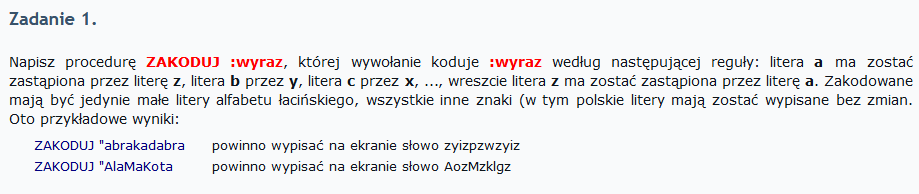
\includegraphics[width=1\linewidth]{./Logia/etap2/1995/zad1.png}
%\end{figure}
%\fromB
%\end{zadanie}
%\begin{zadanie}
%\begin{figure}[H]
%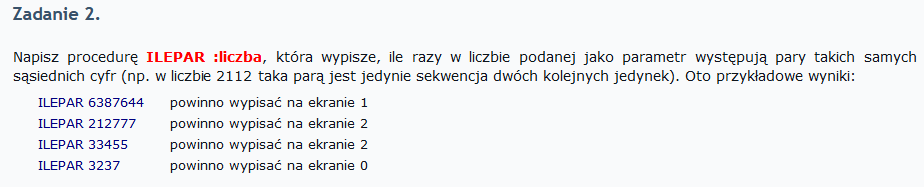
\includegraphics[width=1\linewidth]{./Logia/etap2/1995/zad2.png}
%\end{figure}
%\fromB
%\end{zadanie}
%\begin{zadanie}
%\begin{figure}[H]
%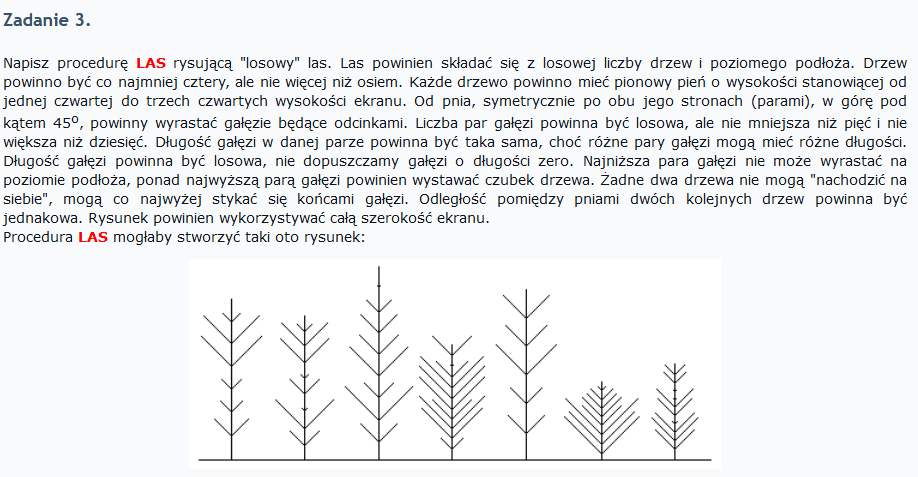
\includegraphics[width=1\linewidth]{./Logia/etap2/1995/zad3.png}
%\end{figure}
%\fromB
%\end{zadanie}
%\begin{zadanie}
%\begin{figure}[H]
%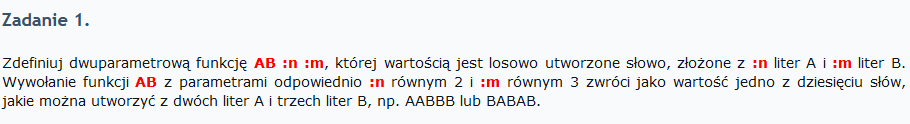
\includegraphics[width=1\linewidth]{./Logia/etap2/1996/zad1.png}
%\end{figure}
%\fromB
%\end{zadanie}
%\begin{zadanie}
%\begin{figure}[H]
%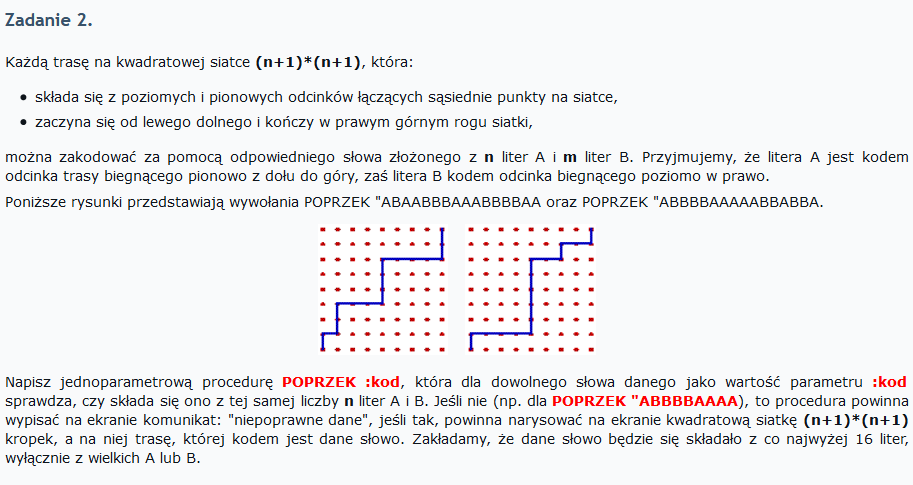
\includegraphics[width=1\linewidth]{./Logia/etap2/1996/zad2.png}
%\end{figure}
%\fromB
%\end{zadanie}
%\begin{zadanie}
%\begin{figure}[H]
%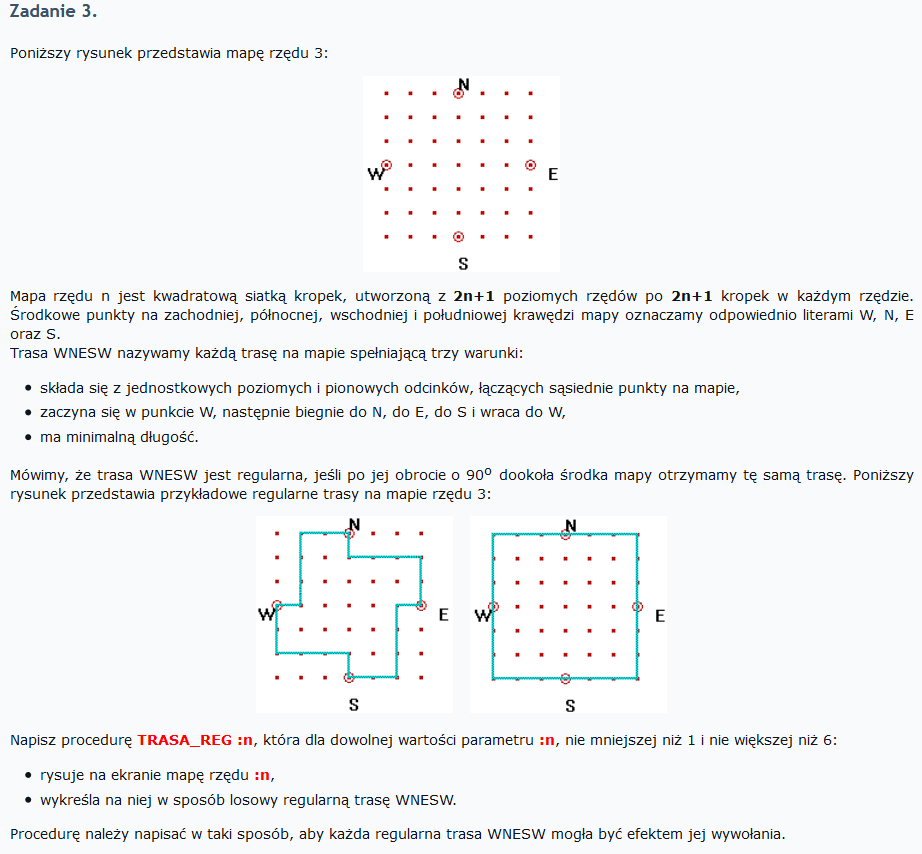
\includegraphics[width=1\linewidth]{./Logia/etap2/1996/zad3.png}
%\end{figure}
%\fromB
%\end{zadanie}
%\begin{zadanie}
%\begin{figure}[H]
%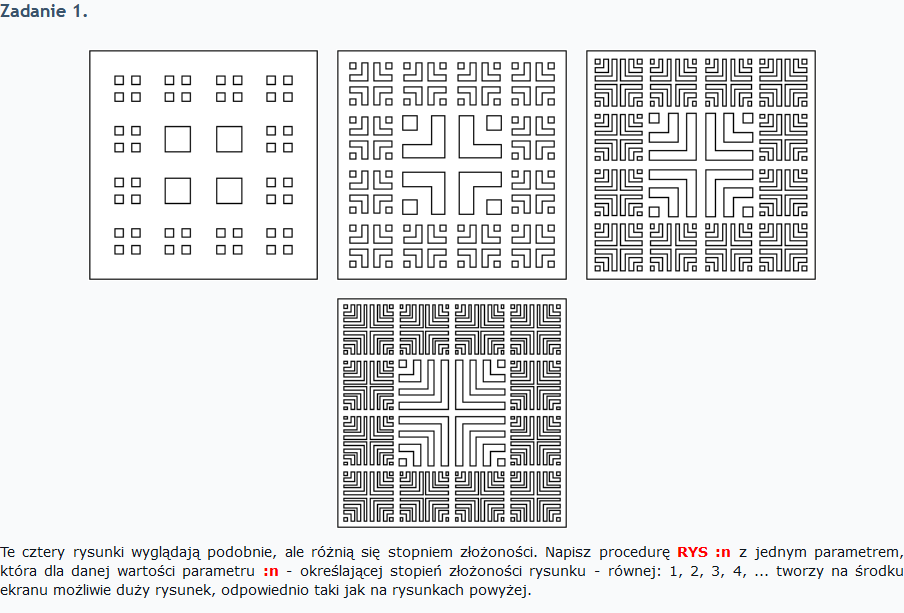
\includegraphics[width=1\linewidth]{./Logia/etap2/1997/zad1.png}
%\end{figure}
%\fromB
%\end{zadanie}
%\begin{zadanie}
%\begin{figure}[H]
%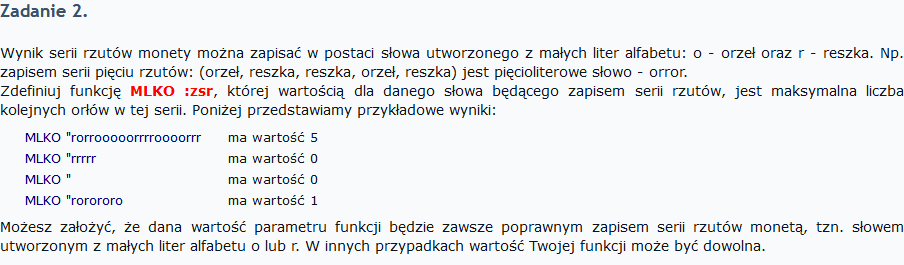
\includegraphics[width=1\linewidth]{./Logia/etap2/1997/zad2.png}
%\end{figure}
%\fromB
%\end{zadanie}
%\begin{zadanie}
%\begin{figure}[H]
%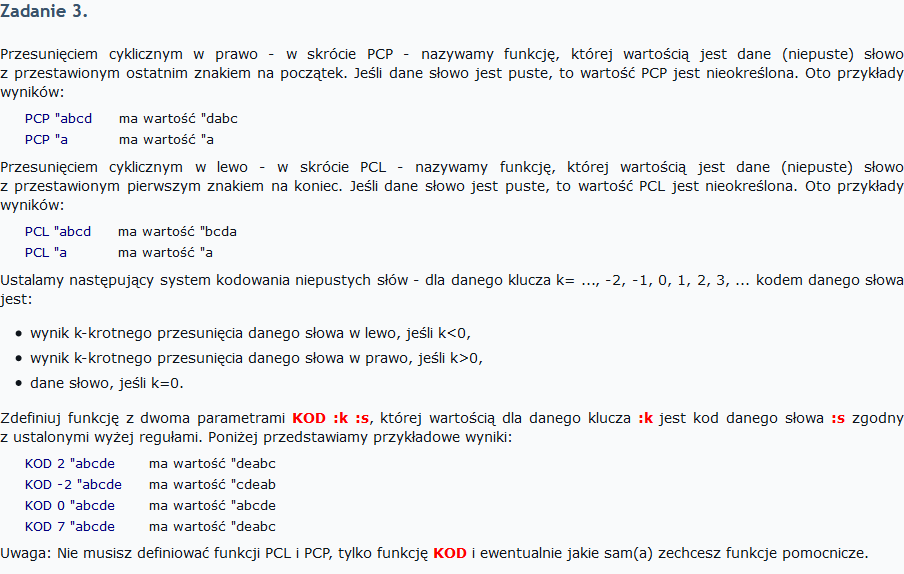
\includegraphics[width=1\linewidth]{./Logia/etap2/1997/zad3.png}
%\end{figure}
%\fromB
%\end{zadanie}
%\begin{zadanie}
%\begin{figure}[H]
%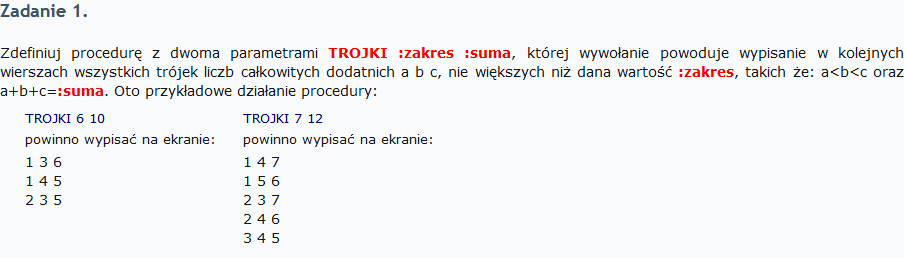
\includegraphics[width=1\linewidth]{./Logia/etap2/1998/zad1.png}
%\end{figure}
%\fromB
%\end{zadanie}
%\begin{zadanie}
%\begin{figure}[H]
%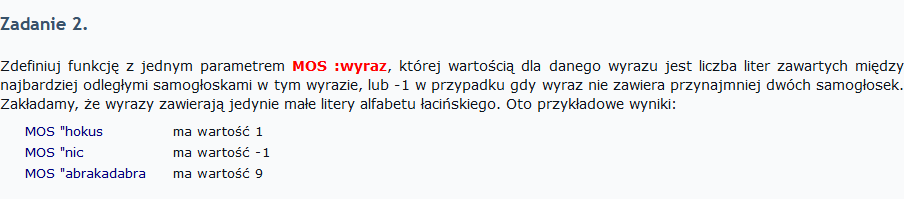
\includegraphics[width=1\linewidth]{./Logia/etap2/1998/zad2.png}
%\end{figure}
%\fromB
%\end{zadanie}
%\begin{zadanie}
%\begin{figure}[H]
%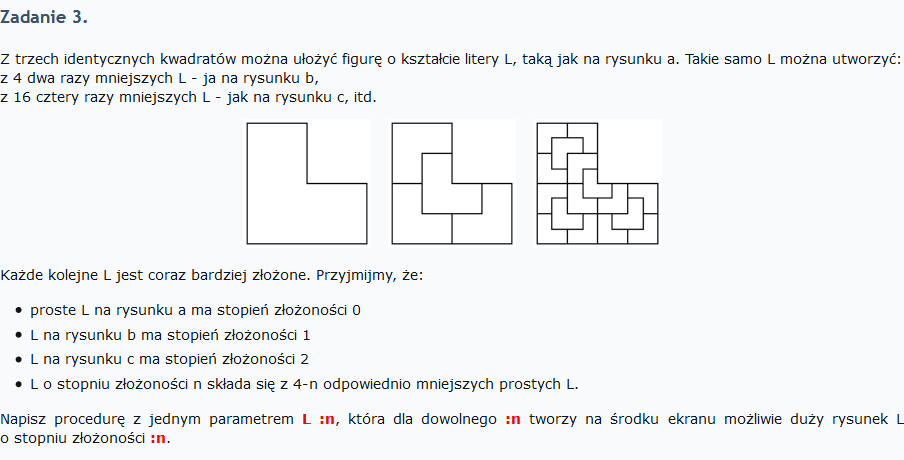
\includegraphics[width=1\linewidth]{./Logia/etap2/1998/zad3.png}
%\end{figure}
%\fromB
%\end{zadanie}
%\begin{zadanie}
%\begin{figure}[H]
%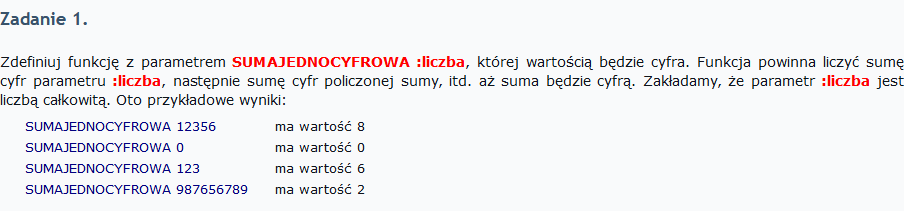
\includegraphics[width=1\linewidth]{./Logia/etap2/1999/zad1.png}
%\end{figure}
%\fromB
%\end{zadanie}
%\begin{zadanie}
%\begin{figure}[H]
%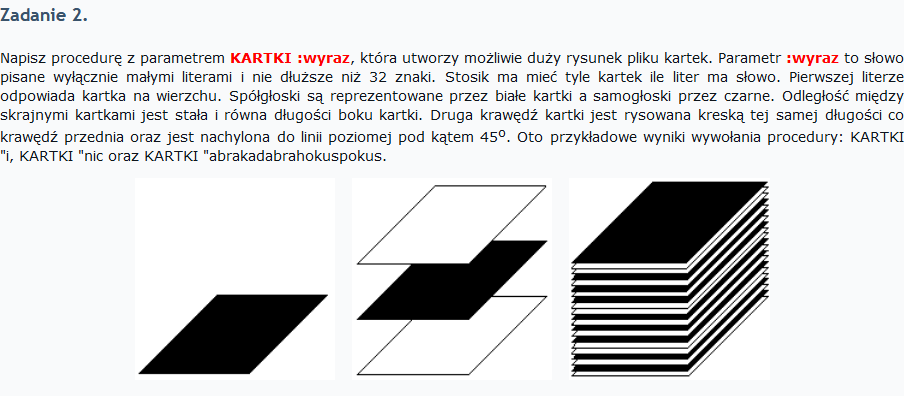
\includegraphics[width=1\linewidth]{./Logia/etap2/1999/zad2.png}
%\end{figure}
%\fromB
%\end{zadanie}
%\begin{zadanie}
%\begin{figure}[H]
%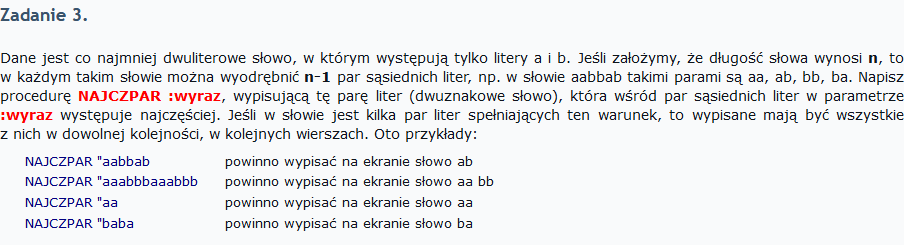
\includegraphics[width=1\linewidth]{./Logia/etap2/1999/zad3.png}
%\end{figure}
%\fromB
%\end{zadanie}
%\begin{zadanie}
%\begin{figure}[H]
%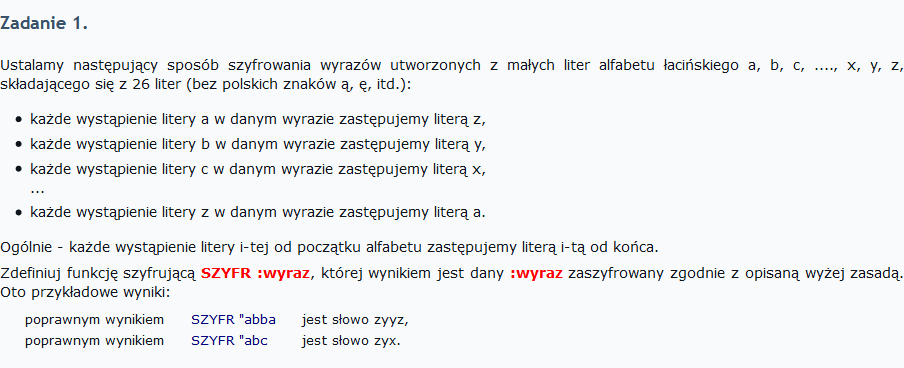
\includegraphics[width=1\linewidth]{./Logia/etap2/2000/zad1.png}
%\end{figure}
%\fromB
%\end{zadanie}
%\begin{zadanie}
%\begin{figure}[H]
%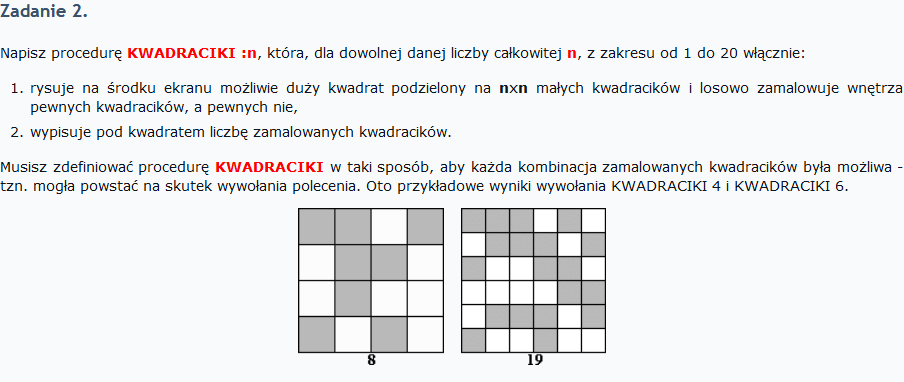
\includegraphics[width=1\linewidth]{./Logia/etap2/2000/zad2.png}
%\end{figure}
%\fromB
%\end{zadanie}
%\begin{zadanie}
%\begin{figure}[H]
%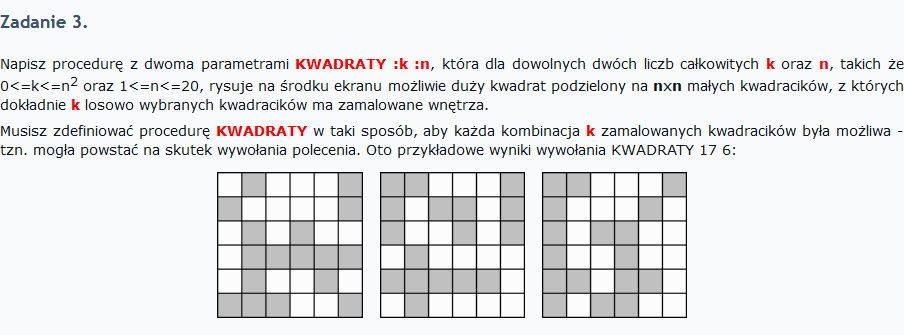
\includegraphics[width=1\linewidth]{./Logia/etap2/2000/zad3.png}
%\end{figure}
%\fromB
%\end{zadanie}
%\begin{zadanie}
%\begin{figure}[H]
%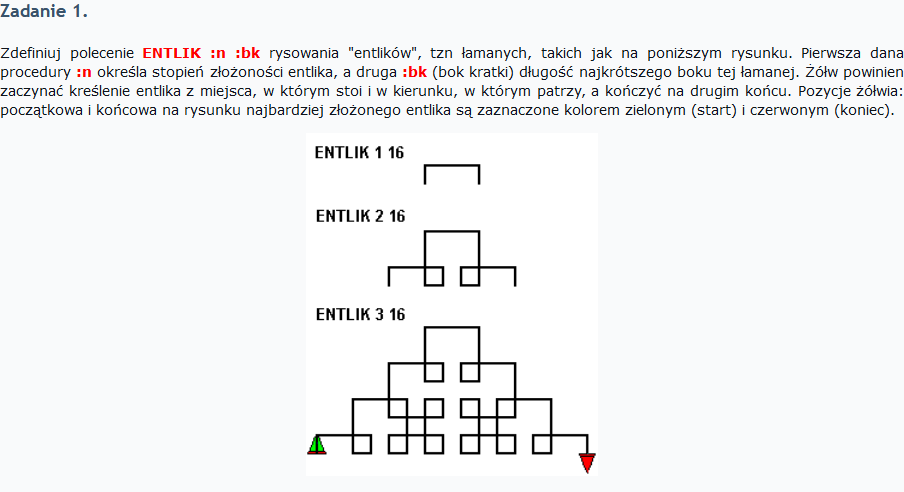
\includegraphics[width=1\linewidth]{./Logia/etap2/2001/zad1.png}
%\end{figure}
%\fromB
%\end{zadanie}
%\begin{zadanie}
%\begin{figure}[H]
%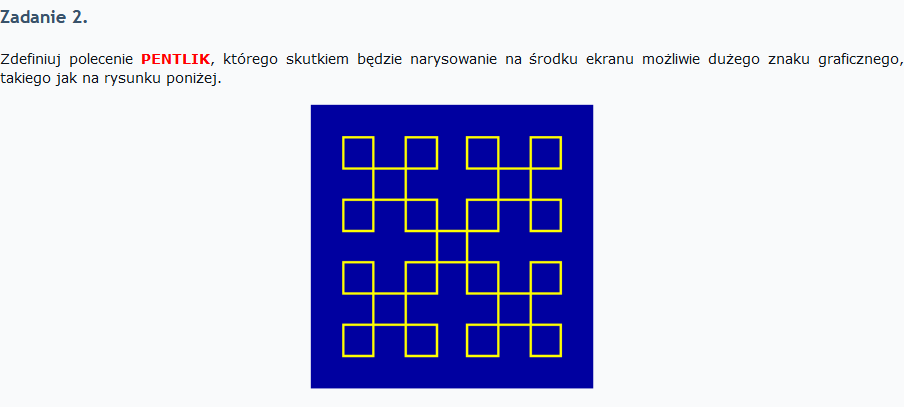
\includegraphics[width=1\linewidth]{./Logia/etap2/2001/zad2.png}
%\end{figure}
%\fromB
%\end{zadanie}
%\begin{zadanie}
%\begin{figure}[H]
%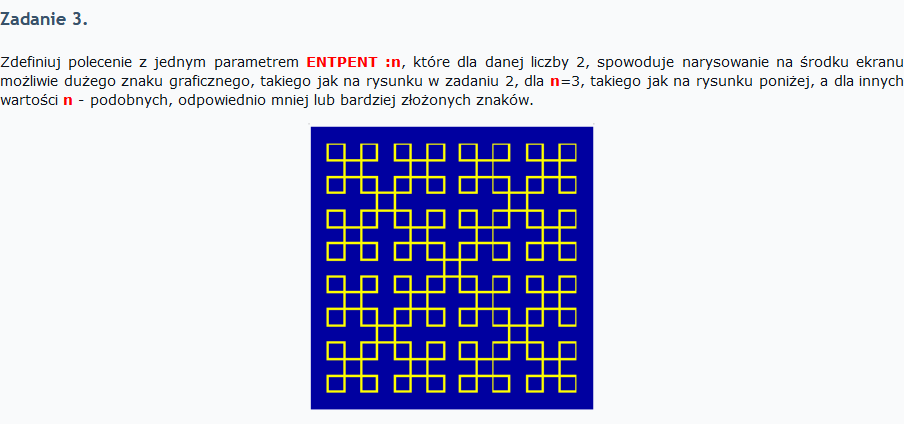
\includegraphics[width=1\linewidth]{./Logia/etap2/2001/zad3.png}
%\end{figure}
%\fromB
%\end{zadanie}
%\begin{zadanie}
%\begin{figure}[H]
%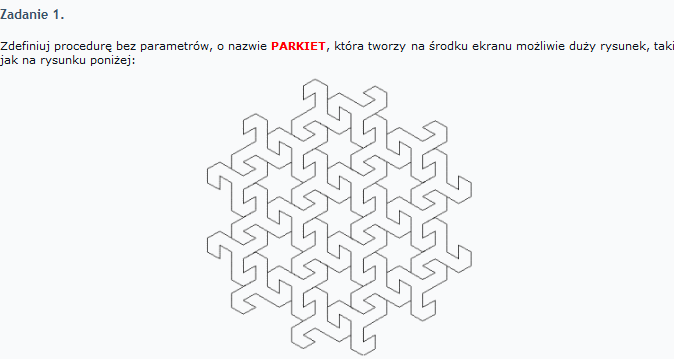
\includegraphics[width=1\linewidth]{./Logia/etap2/2002/zad1.png}
%\end{figure}
%\fromB
%\end{zadanie}
%\begin{zadanie}
%\begin{figure}[H]
%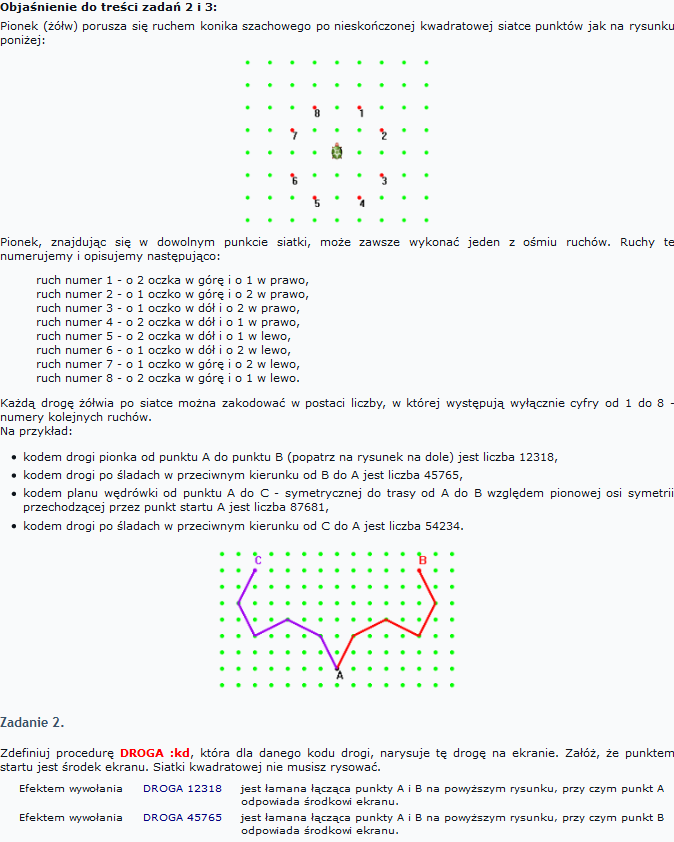
\includegraphics[width=1\linewidth]{./Logia/etap2/2002/zad2.png}
%\end{figure}
%\fromB
%\end{zadanie}
%\begin{zadanie}
%\begin{figure}[H]
%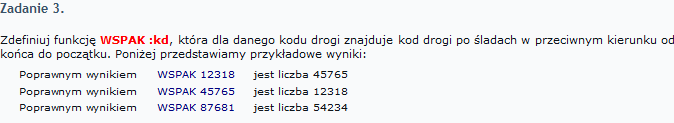
\includegraphics[width=1\linewidth]{./Logia/etap2/2002/zad3.png}
%\end{figure}
%\fromB
%\end{zadanie}
%\begin{zadanie}
%\begin{figure}[H]
%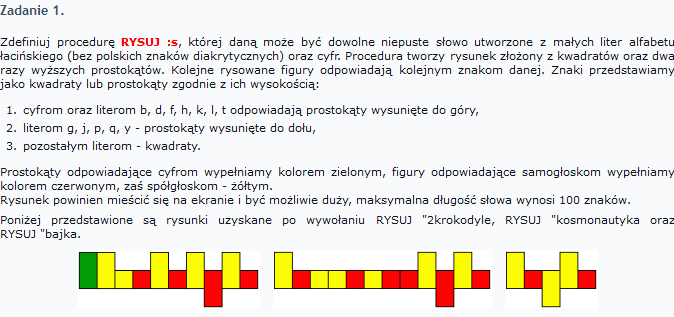
\includegraphics[width=1\linewidth]{./Logia/etap2/2003/zad1.png}
%\end{figure}
%\fromB
%\end{zadanie}
%\begin{zadanie}
%\begin{figure}[H]
%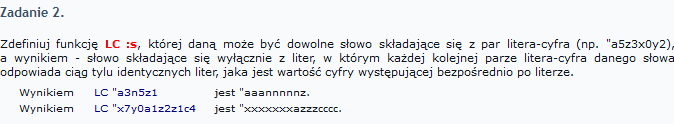
\includegraphics[width=1\linewidth]{./Logia/etap2/2003/zad2.png}
%\end{figure}
%\fromB
%\end{zadanie}
%\begin{zadanie}
%\begin{figure}[H]
%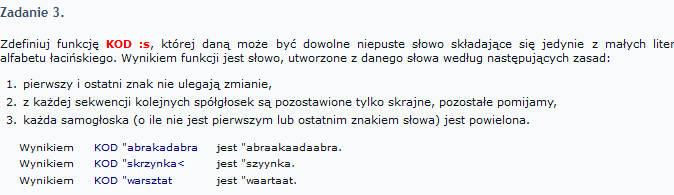
\includegraphics[width=1\linewidth]{./Logia/etap2/2003/zad3.png}
%\end{figure}
%\fromB
%\end{zadanie}
%\begin{zadanie}
%\begin{figure}[H]
%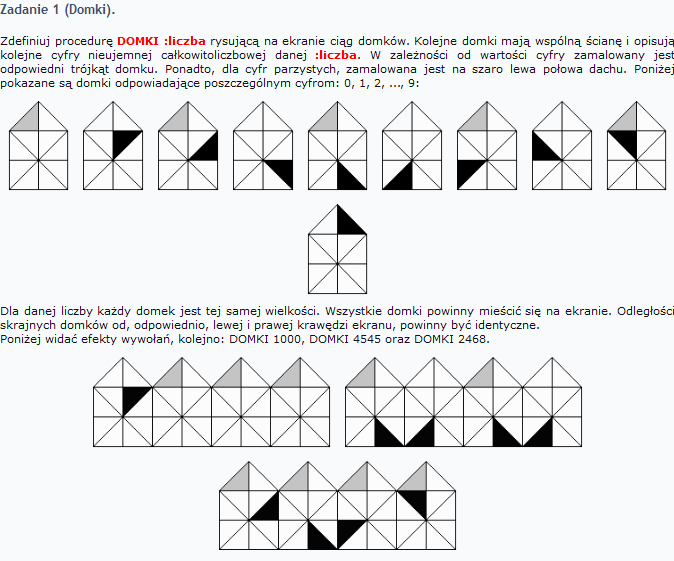
\includegraphics[width=1\linewidth]{./Logia/etap2/2004/zad1.png}
%\end{figure}
%\fromB
%\end{zadanie}
%\begin{zadanie}
%\begin{figure}[H]
%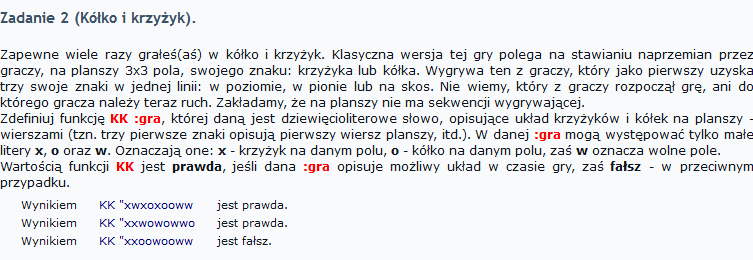
\includegraphics[width=1\linewidth]{./Logia/etap2/2004/zad2.png}
%\end{figure}
%\fromB
%\end{zadanie}
%\begin{zadanie}
%\begin{figure}[H]
%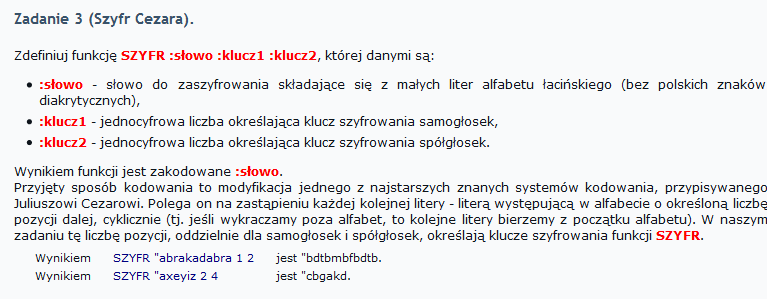
\includegraphics[width=1\linewidth]{./Logia/etap2/2004/zad3.png}
%\end{figure}
%\fromB
%\end{zadanie}
%\begin{zadanie}
%\begin{figure}[H]
%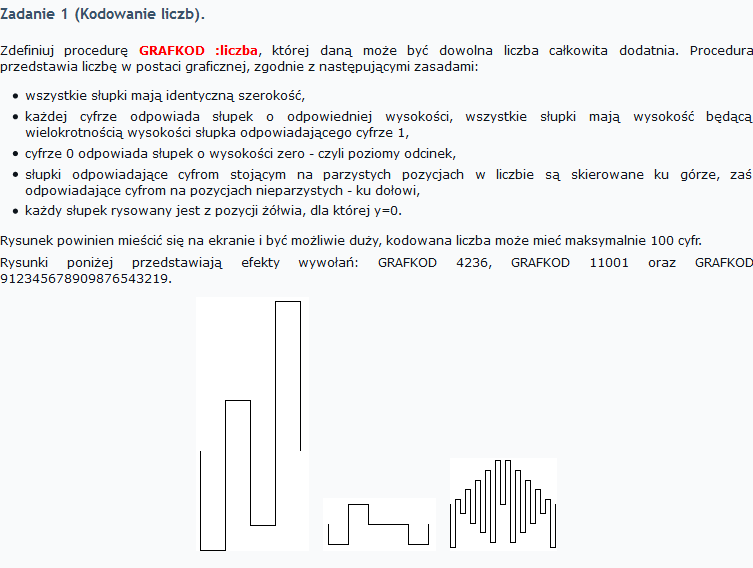
\includegraphics[width=1\linewidth]{./Logia/etap2/2005/zad1.png}
%\end{figure}
%\fromB
%\end{zadanie}
%\begin{zadanie}
%\begin{figure}[H]
%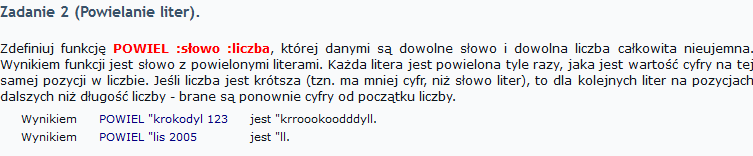
\includegraphics[width=1\linewidth]{./Logia/etap2/2005/zad2.png}
%\end{figure}
%\fromB
%\end{zadanie}
%\begin{zadanie}
%\begin{figure}[H]
%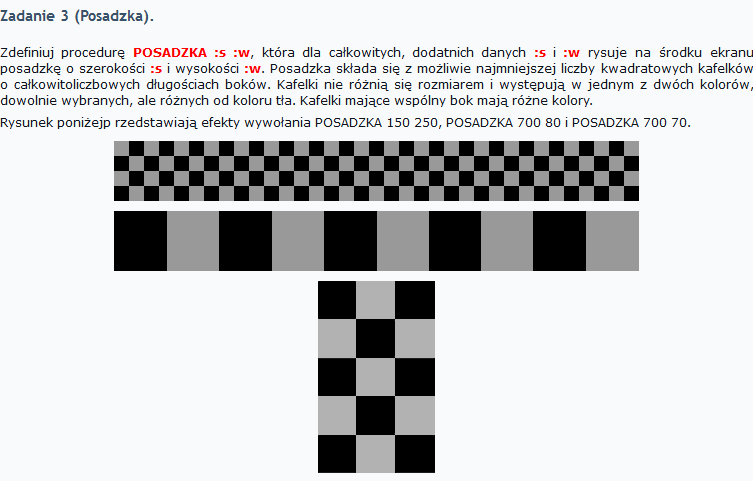
\includegraphics[width=1\linewidth]{./Logia/etap2/2005/zad3.png}
%\end{figure}
%\fromB
%\end{zadanie}
%\begin{zadanie}
%\begin{figure}[H]
%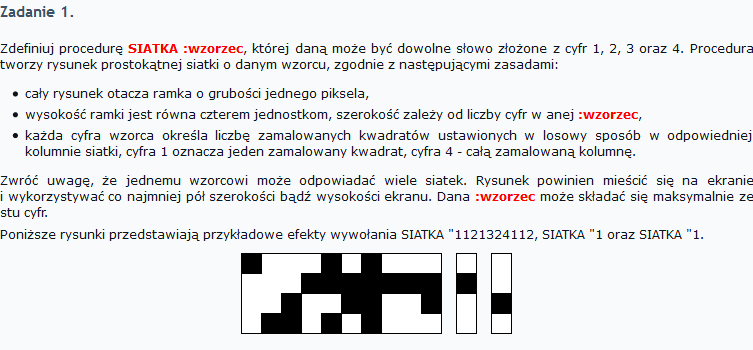
\includegraphics[width=1\linewidth]{./Logia/etap2/2006/zad1.png}
%\end{figure}
%\fromB
%\end{zadanie}
%\begin{zadanie}
%\begin{figure}[H]
%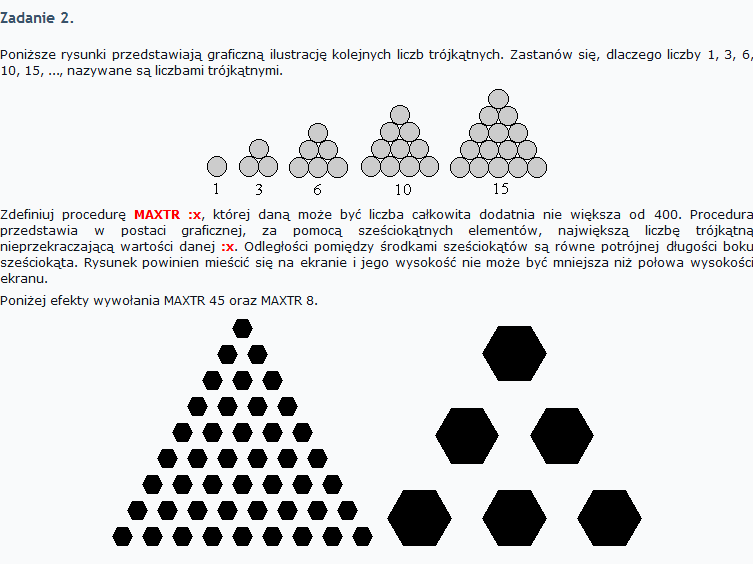
\includegraphics[width=1\linewidth]{./Logia/etap2/2006/zad2.png}
%\end{figure}
%\fromB
%\end{zadanie}
%\begin{zadanie}
%\begin{figure}[H]
%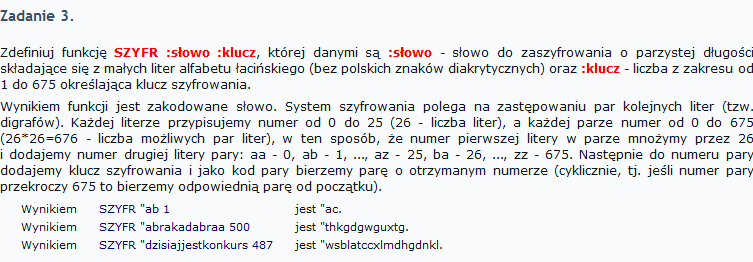
\includegraphics[width=1\linewidth]{./Logia/etap2/2006/zad3.png}
%\end{figure}
%\fromB
%\end{zadanie}
%\begin{zadanie}
%\begin{figure}[H]
%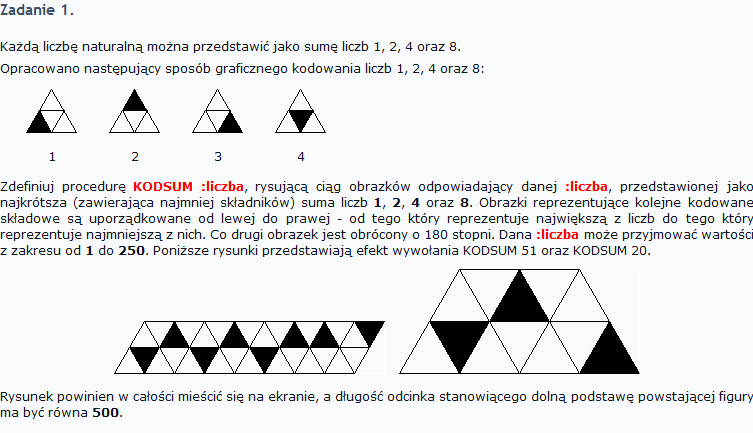
\includegraphics[width=1\linewidth]{./Logia/etap2/2007/zad1.png}
%\end{figure}
%\fromB
%\end{zadanie}
%\begin{zadanie}
%\begin{figure}[H]
%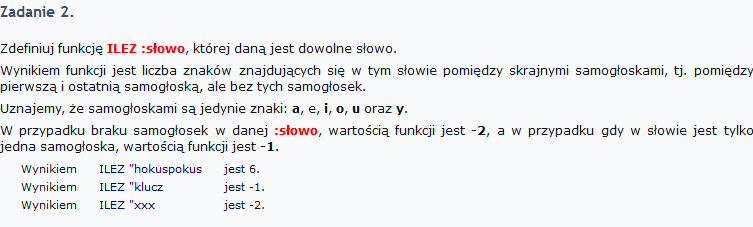
\includegraphics[width=1\linewidth]{./Logia/etap2/2007/zad2.png}
%\end{figure}
%\fromB
%\end{zadanie}
%\begin{zadanie}
%\begin{figure}[H]
%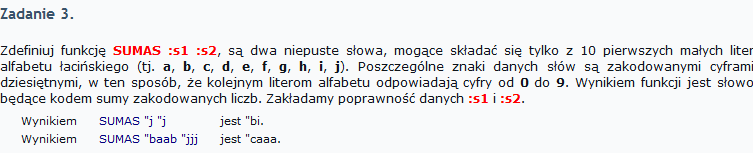
\includegraphics[width=1\linewidth]{./Logia/etap2/2007/zad3.png}
%\end{figure}
%\fromB
%\end{zadanie}
%\begin{zadanie}
%\begin{figure}[H]
%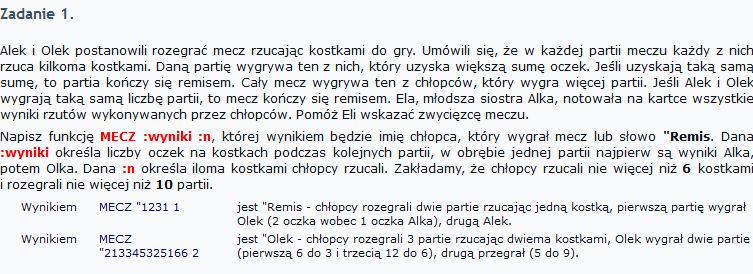
\includegraphics[width=1\linewidth]{./Logia/etap2/2008/zad1.png}
%\end{figure}
%\fromB
%\end{zadanie}
%\begin{zadanie}
%\begin{figure}[H]
%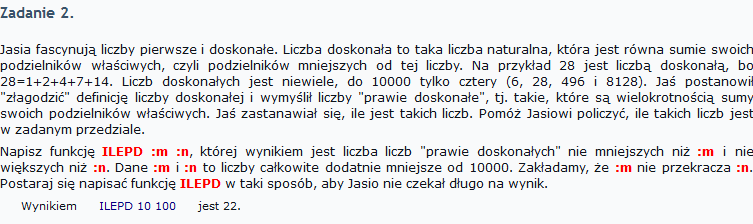
\includegraphics[width=1\linewidth]{./Logia/etap2/2008/zad2.png}
%\end{figure}
%\fromB
%\end{zadanie}
%\begin{zadanie}
%\begin{figure}[H]
%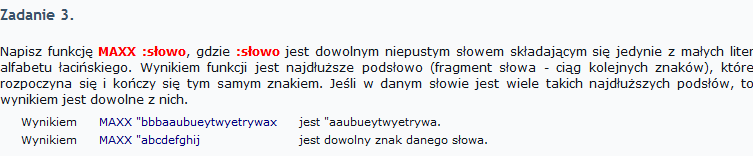
\includegraphics[width=1\linewidth]{./Logia/etap2/2008/zad3.png}
%\end{figure}
%\fromB
%\end{zadanie}
%\begin{zadanie}
%\begin{figure}[H]
%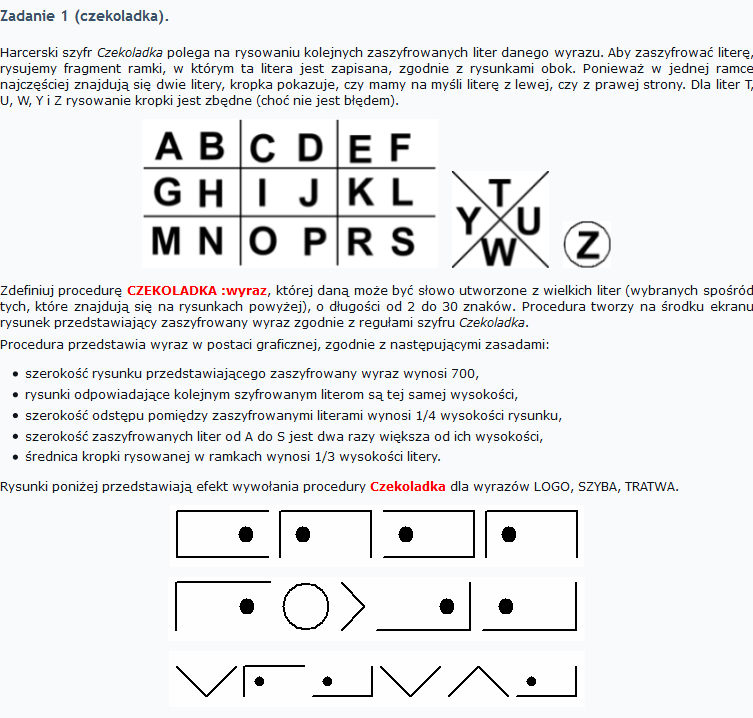
\includegraphics[width=1\linewidth]{./Logia/etap2/2009/zad1.png}
%\end{figure}
%\fromB
%\end{zadanie}
%\begin{zadanie}
%\begin{figure}[H]
%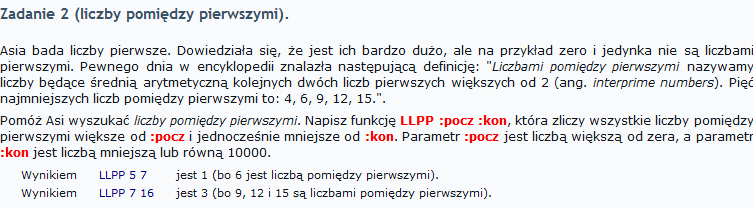
\includegraphics[width=1\linewidth]{./Logia/etap2/2009/zad2.png}
%\end{figure}
%\fromB
%\end{zadanie}
%\begin{zadanie}
%\begin{figure}[H]
%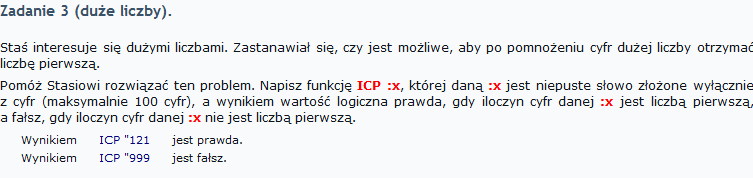
\includegraphics[width=1\linewidth]{./Logia/etap2/2009/zad3.png}
%\end{figure}
%\fromB
%\end{zadanie}
%\begin{zadanie}
%\begin{figure}[H]
%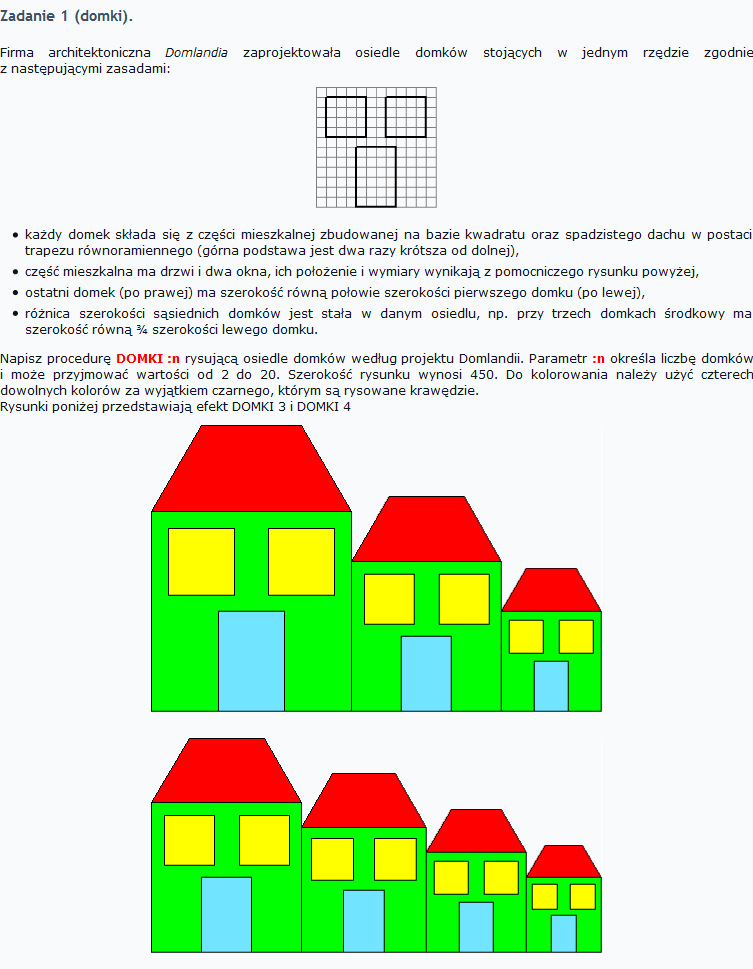
\includegraphics[width=1\linewidth]{./Logia/etap2/2010/zad1.png}
%\end{figure}
%\fromB
%\end{zadanie}
%\begin{zadanie}
%\begin{figure}[H]
%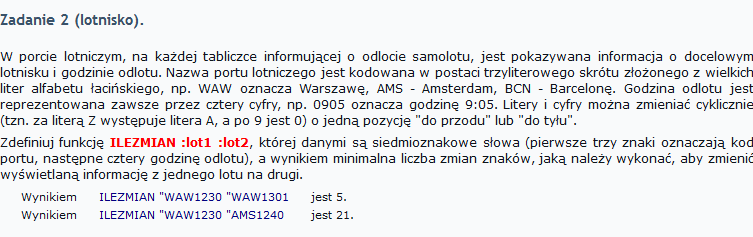
\includegraphics[width=1\linewidth]{./Logia/etap2/2010/zad2.png}
%\end{figure}
%\fromB
%\end{zadanie}
%\begin{zadanie}
%\begin{figure}[H]
%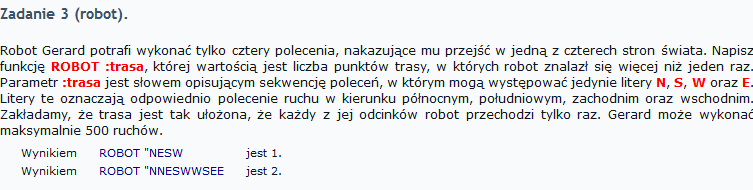
\includegraphics[width=1\linewidth]{./Logia/etap2/2010/zad3.png}
%\end{figure}
%\fromB
%\end{zadanie}
%\begin{zadanie}
%\begin{figure}[H]
%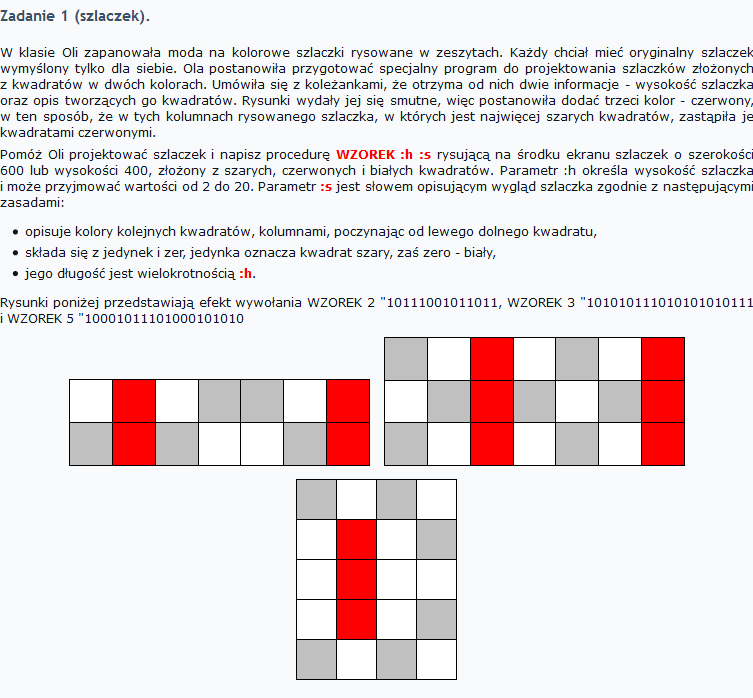
\includegraphics[width=1\linewidth]{./Logia/etap2/2011/zad1.png}
%\end{figure}
%\fromB
%\end{zadanie}
%\begin{zadanie}
%\begin{figure}[H]
%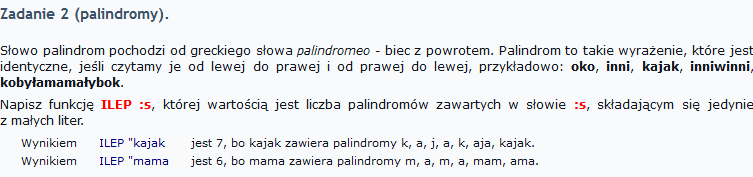
\includegraphics[width=1\linewidth]{./Logia/etap2/2011/zad2.png}
%\end{figure}
%\fromB
%\end{zadanie}
%\begin{zadanie}
%\begin{figure}[H]
%\includegraphics[width=1\linewidth]{./Logia/etap2/2011/zad3.png}
%\end{figure}
%\fromB
%\end{zadanie}
%\begin{zadanie}
%\begin{figure}[H]
%\includegraphics[width=1\linewidth]{./Logia/etap2/2012/zad1.png}
%\end{figure}
%\fromB
%\end{zadanie}
%\begin{zadanie}
%\begin{figure}[H]
%\includegraphics[width=1\linewidth]{./Logia/etap2/2012/zad2.png}
%\end{figure}
%\fromB
%\end{zadanie}
%\begin{zadanie}
%\begin{figure}[H]
%\includegraphics[width=1\linewidth]{./Logia/etap2/2012/zad3.png}
%\end{figure}
%\fromB
%\end{zadanie}
%\begin{zadanie}
%\begin{figure}[H]
%\includegraphics[width=1\linewidth]{./Logia/etap2/2013/zad1.png}
%\end{figure}
%\fromB
%\end{zadanie}
%\begin{zadanie}
%\begin{figure}[H]
%\includegraphics[width=1\linewidth]{./Logia/etap2/2013/zad2.png}
%\end{figure}
%\fromB
%\end{zadanie}
%\begin{zadanie}
%\begin{figure}[H]
%\includegraphics[width=1\linewidth]{./Logia/etap2/2013/zad3.png}
%\end{figure}
%\fromB
%\end{zadanie}
%\begin{zadanie}
%\begin{figure}[H]
%\includegraphics[width=1\linewidth]{./Logia/etap2/2014/zad1.png}
%\end{figure}
%\fromB
%\end{zadanie}
%\begin{zadanie}
%\begin{figure}[H]
%\includegraphics[width=1\linewidth]{./Logia/etap2/2014/zad2.png}
%\end{figure}
%\fromB
%\end{zadanie}
%\begin{zadanie}
%\begin{figure}[H]
%\includegraphics[width=1\linewidth]{./Logia/etap2/2014/zad3.png}
%\end{figure}
%\fromB
%\end{zadanie}
%\begin{zadanie}
%\begin{figure}[H]
%\includegraphics[width=1\linewidth]{./Logia/etap2/2015/zad1.png}
%\end{figure}
%\fromB
%\end{zadanie}
%\begin{zadanie}
%\begin{figure}[H]
%\includegraphics[width=1\linewidth]{./Logia/etap2/2015/zad2.png}
%\end{figure}
%\fromB
%\end{zadanie}
%\begin{zadanie}
%\begin{figure}[H]
%\includegraphics[width=1\linewidth]{./Logia/etap2/2015/zad3.png}
%\end{figure}
%\fromB
%\end{zadanie}
%\begin{zadanie}
%\begin{figure}[H]
%\includegraphics[width=1\linewidth]{./Logia/etap2/2016/zad1.png}
%\end{figure}
%\fromB
%\end{zadanie}
%\begin{zadanie}
%\begin{figure}[H]
%\includegraphics[width=1\linewidth]{./Logia/etap2/2016/zad2.png}
%\end{figure}
%\fromB
%\end{zadanie}
%\begin{zadanie}
%\begin{figure}[H]
%\includegraphics[width=1\linewidth]{./Logia/etap2/2016/zad3.png}
%\end{figure}
%\fromB
%\end{zadanie}
%\begin{zadanie}
%\begin{figure}[H]
%\includegraphics[width=1\linewidth]{./Logia/etap2/2017/zad1.png}
%\end{figure}
%\fromB
%\end{zadanie}
%\begin{zadanie}
%\begin{figure}[H]
%\includegraphics[width=1\linewidth]{./Logia/etap2/2017/zad2.png}
%\end{figure}
%\fromB
%\end{zadanie}
%\begin{zadanie}
%\begin{figure}[H]
%\includegraphics[width=1\linewidth]{./Logia/etap2/2017/zad3.png}
%\end{figure}
%\fromB
%\end{zadanie}
%\begin{zadanie}
%\begin{figure}[H]
%\includegraphics[width=1\linewidth]{./Logia/etap3/1995/zad1.png}
%\end{figure}
%\fromB
%\end{zadanie}
%\begin{zadanie}
%\begin{figure}[H]
%\includegraphics[width=1\linewidth]{./Logia/etap3/1995/zad2.png}
%\end{figure}
%\fromB
%\end{zadanie}
%\begin{zadanie}
%\begin{figure}[H]
%\includegraphics[width=1\linewidth]{./Logia/etap3/1995/zad3.png}
%\end{figure}
%\fromB
%\end{zadanie}
%\begin{zadanie}
%\begin{figure}[H]
%\includegraphics[width=1\linewidth]{./Logia/etap3/1996/zad1.png}
%\end{figure}
%\fromB
%\end{zadanie}
%\begin{zadanie}
%\begin{figure}[H]
%\includegraphics[width=1\linewidth]{./Logia/etap3/1996/zad2.png}
%\end{figure}
%\fromB
%\end{zadanie}
%\begin{zadanie}
%\begin{figure}[H]
%\includegraphics[width=1\linewidth]{./Logia/etap3/1996/zad3.png}
%\end{figure}
%\fromB
%\end{zadanie}
%\begin{zadanie}
%\begin{figure}[H]
%\includegraphics[width=1\linewidth]{./Logia/etap3/1997/zad1.png}
%\end{figure}
%\fromB
%\end{zadanie}
%\begin{zadanie}
%\begin{figure}[H]
%\includegraphics[width=1\linewidth]{./Logia/etap3/1997/zad2.png}
%\end{figure}
%\fromB
%\end{zadanie}
%\begin{zadanie}
%\begin{figure}[H]
%\includegraphics[width=1\linewidth]{./Logia/etap3/1997/zad3.png}
%\end{figure}
%\fromB
%\end{zadanie}
%\begin{zadanie}
%\begin{figure}[H]
%\includegraphics[width=1\linewidth]{./Logia/etap3/1998/zad1.png}
%\end{figure}
%\fromB
%\end{zadanie}
%\begin{zadanie}
%\begin{figure}[H]
%\includegraphics[width=1\linewidth]{./Logia/etap3/1998/zad2.png}
%\end{figure}
%\fromB
%\end{zadanie}
%\begin{zadanie}
%\begin{figure}[H]
%\includegraphics[width=1\linewidth]{./Logia/etap3/1998/zad3.png}
%\end{figure}
%\fromB
%\end{zadanie}
%\begin{zadanie}
%\begin{figure}[H]
%\includegraphics[width=1\linewidth]{./Logia/etap3/1999/zad1.png}
%\end{figure}
%\fromB
%\end{zadanie}
%\begin{zadanie}
%\begin{figure}[H]
%\includegraphics[width=1\linewidth]{./Logia/etap3/1999/zad2.png}
%\end{figure}
%\fromB
%\end{zadanie}
%\begin{zadanie}
%\begin{figure}[H]
%\includegraphics[width=1\linewidth]{./Logia/etap3/1999/zad3.png}
%\end{figure}
%\fromB
%\end{zadanie}
%\begin{zadanie}
%\begin{figure}[H]
%\includegraphics[width=1\linewidth]{./Logia/etap3/2000/zad1.png}
%\end{figure}
%\fromB
%\end{zadanie}
%\begin{zadanie}
%\begin{figure}[H]
%\includegraphics[width=1\linewidth]{./Logia/etap3/2000/zad2.png}
%\end{figure}
%\fromB
%\end{zadanie}
%\begin{zadanie}
%\begin{figure}[H]
%\includegraphics[width=1\linewidth]{./Logia/etap3/2000/zad3.png}
%\end{figure}
%\fromB
%\end{zadanie}
%\begin{zadanie}
%\begin{figure}[H]
%\includegraphics[width=1\linewidth]{./Logia/etap3/2001/zad0.png}
%\end{figure}
%\fromB
%\end{zadanie}
%\begin{zadanie}
%\begin{figure}[H]
%\includegraphics[width=1\linewidth]{./Logia/etap3/2001/zad1.png}
%\end{figure}
%\fromB
%\end{zadanie}
%\begin{zadanie}
%\begin{figure}[H]
%\includegraphics[width=1\linewidth]{./Logia/etap3/2001/zad2.png}
%\end{figure}
%\fromB
%\end{zadanie}
%\begin{zadanie}
%\begin{figure}[H]
%\includegraphics[width=1\linewidth]{./Logia/etap3/2001/zad3.png}
%\end{figure}
%\fromB
%\end{zadanie}
%\begin{zadanie}
%\begin{figure}[H]
%\includegraphics[width=1\linewidth]{./Logia/etap3/2001/zad4.png}
%\end{figure}
%\fromB
%\end{zadanie}
%\begin{zadanie}
%\begin{figure}[H]
%\includegraphics[width=1\linewidth]{./Logia/etap3/2002/zad0.png}
%\end{figure}
%\fromB
%\end{zadanie}
%\begin{zadanie}
%\begin{figure}[H]
%\includegraphics[width=1\linewidth]{./Logia/etap3/2002/zad1.png}
%\end{figure}
%\fromB
%\end{zadanie}
%\begin{zadanie}
%\begin{figure}[H]
%\includegraphics[width=1\linewidth]{./Logia/etap3/2002/zad2.png}
%\end{figure}
%\fromB
%\end{zadanie}
%\begin{zadanie}
%\begin{figure}[H]
%\includegraphics[width=1\linewidth]{./Logia/etap3/2002/zad3.png}
%\end{figure}
%\fromB
%\end{zadanie}
%\begin{zadanie}
%\begin{figure}[H]
%\includegraphics[width=1\linewidth]{./Logia/etap3/2002/zad4.png}
%\end{figure}
%\fromB
%\end{zadanie}
%\begin{zadanie}
%\begin{figure}[H]
%\includegraphics[width=1\linewidth]{./Logia/etap3/2003/zad1.png}
%\end{figure}
%\fromB
%\end{zadanie}
%\begin{zadanie}
%\begin{figure}[H]
%\includegraphics[width=1\linewidth]{./Logia/etap3/2003/zad2.png}
%\end{figure}
%\fromB
%\end{zadanie}
%\begin{zadanie}
%\begin{figure}[H]
%\includegraphics[width=1\linewidth]{./Logia/etap3/2003/zad3.png}
%\end{figure}
%\fromB
%\end{zadanie}
%\begin{zadanie}
%\begin{figure}[H]
%\includegraphics[width=1\linewidth]{./Logia/etap3/2003/zad4.png}
%\end{figure}
%\fromB
%\end{zadanie}
%\begin{zadanie}
%\begin{figure}[H]
%\includegraphics[width=1\linewidth]{./Logia/etap3/2004/zad1.png}
%\end{figure}
%\fromB
%\end{zadanie}
%\begin{zadanie}
%\begin{figure}[H]
%\includegraphics[width=1\linewidth]{./Logia/etap3/2004/zad2.png}
%\end{figure}
%\fromB
%\end{zadanie}
%\begin{zadanie}
%\begin{figure}[H]
%\includegraphics[width=1\linewidth]{./Logia/etap3/2004/zad3.png}
%\end{figure}
%\fromB
%\end{zadanie}
%\begin{zadanie}
%\begin{figure}[H]
%\includegraphics[width=1\linewidth]{./Logia/etap3/2004/zad4.png}
%\end{figure}
%\fromB
%\end{zadanie}
%\begin{zadanie}
%\begin{figure}[H]
%\includegraphics[width=1\linewidth]{./Logia/etap3/2005/zad1.png}
%\end{figure}
%\fromB
%\end{zadanie}
%\begin{zadanie}
%\begin{figure}[H]
%\includegraphics[width=1\linewidth]{./Logia/etap3/2005/zad2.png}
%\end{figure}
%\fromB
%\end{zadanie}
%\begin{zadanie}
%\begin{figure}[H]
%\includegraphics[width=1\linewidth]{./Logia/etap3/2005/zad3.png}
%\end{figure}
%\fromB
%\end{zadanie}
%\begin{zadanie}
%\begin{figure}[H]
%\includegraphics[width=1\linewidth]{./Logia/etap3/2005/zad4.png}
%\end{figure}
%\fromB
%\end{zadanie}
%\begin{zadanie}
%\begin{figure}[H]
%\includegraphics[width=1\linewidth]{./Logia/etap3/2006/zad1.png}
%\end{figure}
%\fromB
%\end{zadanie}
%\begin{zadanie}
%\begin{figure}[H]
%\includegraphics[width=1\linewidth]{./Logia/etap3/2006/zad2.png}
%\end{figure}
%\fromB
%\end{zadanie}
%\begin{zadanie}
%\begin{figure}[H]
%\includegraphics[width=1\linewidth]{./Logia/etap3/2006/zad3.png}
%\end{figure}
%\fromB
%\end{zadanie}
%\begin{zadanie}
%\begin{figure}[H]
%\includegraphics[width=1\linewidth]{./Logia/etap3/2006/zad4.png}
%\end{figure}
%\fromB
%\end{zadanie}
%\begin{zadanie}
%\begin{figure}[H]
%\includegraphics[width=1\linewidth]{./Logia/etap3/2007/zad1.png}
%\end{figure}
%\fromB
%\end{zadanie}
%\begin{zadanie}
%\begin{figure}[H]
%\includegraphics[width=1\linewidth]{./Logia/etap3/2007/zad2.png}
%\end{figure}
%\fromB
%\end{zadanie}
%\begin{zadanie}
%\begin{figure}[H]
%\includegraphics[width=1\linewidth]{./Logia/etap3/2007/zad3.png}
%\end{figure}
%\fromB
%\end{zadanie}
%\begin{zadanie}
%\begin{figure}[H]
%\includegraphics[width=1\linewidth]{./Logia/etap3/2007/zad4.png}
%\end{figure}
%\fromB
%\end{zadanie}
%\begin{zadanie}
%\begin{figure}[H]
%\includegraphics[width=1\linewidth]{./Logia/etap3/2008/zad1.png}
%\end{figure}
%\fromB
%\end{zadanie}
%\begin{zadanie}
%\begin{figure}[H]
%\includegraphics[width=1\linewidth]{./Logia/etap3/2008/zad2.png}
%\end{figure}
%\fromB
%\end{zadanie}
%\begin{zadanie}
%\begin{figure}[H]
%\includegraphics[width=1\linewidth]{./Logia/etap3/2008/zad3.png}
%\end{figure}
%\fromB
%\end{zadanie}
%\begin{zadanie}
%\begin{figure}[H]
%\includegraphics[width=1\linewidth]{./Logia/etap3/2008/zad4.png}
%\end{figure}
%\fromB
%\end{zadanie}
%\begin{zadanie}
%\begin{figure}[H]
%\includegraphics[width=1\linewidth]{./Logia/etap3/2009/zad1.png}
%\end{figure}
%\fromB
%\end{zadanie}
%\begin{zadanie}
%\begin{figure}[H]
%\includegraphics[width=1\linewidth]{./Logia/etap3/2009/zad2.png}
%\end{figure}
%\fromB
%\end{zadanie}
%\begin{zadanie}
%\begin{figure}[H]
%\includegraphics[width=1\linewidth]{./Logia/etap3/2009/zad3.png}
%\end{figure}
%\fromB
%\end{zadanie}
%\begin{zadanie}
%\begin{figure}[H]
%\includegraphics[width=1\linewidth]{./Logia/etap3/2009/zad4.png}
%\end{figure}
%\fromB
%\end{zadanie}
%\begin{zadanie}
%\begin{figure}[H]
%\includegraphics[width=1\linewidth]{./Logia/etap3/2010/zad1.png}
%\end{figure}
%\fromB
%\end{zadanie}
%\begin{zadanie}
%\begin{figure}[H]
%\includegraphics[width=1\linewidth]{./Logia/etap3/2010/zad2.png}
%\end{figure}
%\fromB
%\end{zadanie}
%\begin{zadanie}
%\begin{figure}[H]
%\includegraphics[width=1\linewidth]{./Logia/etap3/2010/zad3.png}
%\end{figure}
%\fromB
%\end{zadanie}
%\begin{zadanie}
%\begin{figure}[H]
%\includegraphics[width=1\linewidth]{./Logia/etap3/2010/zad4.png}
%\end{figure}
%\fromB
%\end{zadanie}
%\begin{zadanie}
%\begin{figure}[H]
%\includegraphics[width=1\linewidth]{./Logia/etap3/2011/zad1.png}
%\end{figure}
%\fromB
%\end{zadanie}
%\begin{zadanie}
%\begin{figure}[H]
%\includegraphics[width=1\linewidth]{./Logia/etap3/2011/zad2.png}
%\end{figure}
%\fromB
%\end{zadanie}
%\begin{zadanie}
%\begin{figure}[H]
%\includegraphics[width=1\linewidth]{./Logia/etap3/2011/zad3.png}
%\end{figure}
%\fromB
%\end{zadanie}
%\begin{zadanie}
%\begin{figure}[H]
%\includegraphics[width=1\linewidth]{./Logia/etap3/2011/zad4.png}
%\end{figure}
%\fromB
%\end{zadanie}
%\begin{zadanie}
%\begin{figure}[H]
%\includegraphics[width=1\linewidth]{./Logia/etap3/2012/zad1.png}
%\end{figure}
%\fromB
%\end{zadanie}
%\begin{zadanie}
%\begin{figure}[H]
%\includegraphics[width=1\linewidth]{./Logia/etap3/2012/zad2.png}
%\end{figure}
%\fromB
%\end{zadanie}
%\begin{zadanie}
%\begin{figure}[H]
%\includegraphics[width=1\linewidth]{./Logia/etap3/2012/zad3.png}
%\end{figure}
%\fromB
%\end{zadanie}
%\begin{zadanie}
%\begin{figure}[H]
%\includegraphics[width=1\linewidth]{./Logia/etap3/2012/zad4.png}
%\end{figure}
%\fromB
%\end{zadanie}
%\begin{zadanie}
%\begin{figure}[H]
%\includegraphics[width=1\linewidth]{./Logia/etap3/2013/zad1.png}
%\end{figure}
%\fromB
%\end{zadanie}
%\begin{zadanie}
%\begin{figure}[H]
%\includegraphics[width=1\linewidth]{./Logia/etap3/2013/zad2.png}
%\end{figure}
%\fromB
%\end{zadanie}
%\begin{zadanie}
%\begin{figure}[H]
%\includegraphics[width=1\linewidth]{./Logia/etap3/2013/zad3.png}
%\end{figure}
%\fromB
%\end{zadanie}
%\begin{zadanie}
%\begin{figure}[H]
%\includegraphics[width=1\linewidth]{./Logia/etap3/2013/zad4.png}
%\end{figure}
%\fromB
%\end{zadanie}
%\begin{zadanie}
%\begin{figure}[H]
%\includegraphics[width=1\linewidth]{./Logia/etap3/2014/zad1.png}
%\end{figure}
%\fromB
%\end{zadanie}
%\begin{zadanie}
%\begin{figure}[H]
%\includegraphics[width=1\linewidth]{./Logia/etap3/2014/zad2.png}
%\end{figure}
%\fromB
%\end{zadanie}
%\begin{zadanie}
%\begin{figure}[H]
%\includegraphics[width=1\linewidth]{./Logia/etap3/2014/zad3.png}
%\end{figure}
%\fromB
%\end{zadanie}
%\begin{zadanie}
%\begin{figure}[H]
%\includegraphics[width=1\linewidth]{./Logia/etap3/2014/zad4.png}
%\end{figure}
%\fromB
%\end{zadanie}
%\begin{zadanie}
%\begin{figure}[H]
%\includegraphics[width=1\linewidth]{./Logia/etap3/2015/zad1.png}
%\end{figure}
%\fromB
%\end{zadanie}
%\begin{zadanie}
%\begin{figure}[H]
%\includegraphics[width=1\linewidth]{./Logia/etap3/2015/zad2.png}
%\end{figure}
%\fromB
%\end{zadanie}
%\begin{zadanie}
%\begin{figure}[H]
%\includegraphics[width=1\linewidth]{./Logia/etap3/2015/zad3.png}
%\end{figure}
%\fromB
%\end{zadanie}
%\begin{zadanie}
%\begin{figure}[H]
%\includegraphics[width=1\linewidth]{./Logia/etap3/2015/zad4.png}
%\end{figure}
%\fromB
%\end{zadanie}
%\begin{zadanie}
%\begin{figure}[H]
%\includegraphics[width=1\linewidth]{./Logia/etap3/2016/zad1.png}
%\end{figure}
%\fromB
%\end{zadanie}
%\begin{zadanie}
%\begin{figure}[H]
%\includegraphics[width=1\linewidth]{./Logia/etap3/2016/zad2.png}
%\end{figure}
%\fromB
%\end{zadanie}
%\begin{zadanie}
%\begin{figure}[H]
%\includegraphics[width=1\linewidth]{./Logia/etap3/2016/zad3.png}
%\end{figure}
%\fromB
%\end{zadanie}
%\begin{zadanie}
%\begin{figure}[H]
%\includegraphics[width=1\linewidth]{./Logia/etap3/2016/zad4.png}
%\end{figure}
%\fromB
%\end{zadanie}
%\begin{zadanie}
%\begin{figure}[H]
%\includegraphics[width=1\linewidth]{./Logia/etap3/2017/zad1.png}
%\end{figure}
%\fromB
%\end{zadanie}
%\begin{zadanie}
%\begin{figure}[H]
%\includegraphics[width=1\linewidth]{./Logia/etap3/2017/zad2.png}
%\end{figure}
%\fromB
%\end{zadanie}
%\begin{zadanie}
%\begin{figure}[H]
%\includegraphics[width=1\linewidth]{./Logia/etap3/2017/zad3.png}
%\end{figure}
%\fromB
%\end{zadanie}
%\begin{zadanie}
%\begin{figure}[H]
%\includegraphics[width=1\linewidth]{./Logia/etap3/2017/zad4.png}
%\end{figure}
%\fromB
%\end{zadanie}
%
%\section{Zadania 3}
%
%\begin{zadanie}
%\includepdf{./OIG/adas.pdf}
%\end{zadanie}
%\begin{zadanie}
%\includepdf{./OIG/and.pdf}
%\end{zadanie}
%\begin{zadanie}
%\includepdf{./OIG/anteny.pdf}
%\end{zadanie}
%\begin{zadanie}
%\includepdf{./OIG/aptzad.pdf}
%\end{zadanie}
%\begin{zadanie}
%\includepdf{./OIG/awaria.pdf}
%\end{zadanie}
%\begin{zadanie}
%\includepdf{./OIG/awariaRakiety.pdf}
%\end{zadanie}
%\begin{zadanie}
%\includepdf{./OIG/a_konik.pdf}
%\end{zadanie}
%\begin{zadanie}
%\includepdf{./OIG/a_palindrom.pdf}
%\end{zadanie}
%\begin{zadanie}
%\includepdf{./OIG/bank.pdf}
%\end{zadanie}
%\begin{zadanie}
%\includepdf{./OIG/blizniaki.pdf}
%\end{zadanie}
%\begin{zadanie}
%\includepdf{./OIG/boig.pdf}
%\end{zadanie}
%\begin{zadanie}
%\includepdf{./OIG/boisko.pdf}
%\end{zadanie}
%\begin{zadanie}
%\includepdf{./OIG/bonifacy.pdf}
%\end{zadanie}
%\begin{zadanie}
%\includepdf{./OIG/bungee.pdf}
%\end{zadanie}
%\begin{zadanie}
%\includepdf{./OIG/bunkry.pdf}
%\end{zadanie}
%\begin{zadanie}
%\includepdf{./OIG/b_skrzynie.pdf}
%\end{zadanie}
%\begin{zadanie}
%\includepdf{./OIG/b_srednia.pdf}
%\end{zadanie}
%\begin{zadanie}
%\includepdf{./OIG/centrum.pdf}
%\end{zadanie}
%\begin{zadanie}
%\includepdf{./OIG/chlopiec.pdf}
%\end{zadanie}
%\begin{zadanie}
%\includepdf{./OIG/cia.pdf}
%\end{zadanie}
%\begin{zadanie}
%\includepdf{./OIG/ciag.pdf}
%\end{zadanie}
%\begin{zadanie}
%\includepdf{./OIG/ciagi.pdf}
%\end{zadanie}
%\begin{zadanie}
%\includepdf{./OIG/ciezarek.pdf}
%\end{zadanie}
%\begin{zadanie}
%\includepdf{./OIG/cukierki.pdf}
%\end{zadanie}
%\begin{zadanie}
%\includepdf{./OIG/czw.pdf}
%\end{zadanie}
%\begin{zadanie}
%\includepdf{./OIG/c_dach.pdf}
%\end{zadanie}
%\begin{zadanie}
%\includepdf{./OIG/c_trudnosc.pdf}
%\end{zadanie}
%\begin{zadanie}
%\includepdf{./OIG/dab.pdf}
%\end{zadanie}
%\begin{zadanie}
%\includepdf{./OIG/dac.pdf}
%\end{zadanie}
%\begin{zadanie}
%\includepdf{./OIG/diamenty.pdf}
%\end{zadanie}
%\begin{zadanie}
%\includepdf{./OIG/domino.pdf}
%\end{zadanie}
%\begin{zadanie}
%\includepdf{./OIG/doskonale.pdf}
%\end{zadanie}
%\begin{zadanie}
%\includepdf{./OIG/doswiadczenie.pdf}
%\end{zadanie}
%\begin{zadanie}
%\includepdf{./OIG/drukarka.pdf}
%\end{zadanie}
%\begin{zadanie}
%\includepdf{./OIG/drzewa.pdf}
%\end{zadanie}
%\begin{zadanie}
%\includepdf{./OIG/drzewo.pdf}
%\end{zadanie}
%\begin{zadanie}
%\includepdf{./OIG/dwazad.pdf}
%\end{zadanie}
%\begin{zadanie}
%\includepdf{./OIG/dwunim.pdf}
%\end{zadanie}
%\begin{zadanie}
%\includepdf{./OIG/dwupalindrom.pdf}
%\end{zadanie}
%\begin{zadanie}
%\includepdf{./OIG/dwuwymiarowe.pdf}
%\end{zadanie}
%\begin{zadanie}
%\includepdf{./OIG/dzieci.pdf}
%\end{zadanie}
%\begin{zadanie}
%\includepdf{./OIG/dzwig.pdf}
%\end{zadanie}
%\begin{zadanie}
%\includepdf{./OIG/d_drzewka.pdf}
%\end{zadanie}
%\begin{zadanie}
%\includepdf{./OIG/d_euklides.pdf}
%\end{zadanie}
%\begin{zadanie}
%\includepdf{./OIG/e_grzegorz.pdf}
%\end{zadanie}
%\begin{zadanie}
%\includepdf{./OIG/e_kamien.pdf}
%\end{zadanie}
%\begin{zadanie}
%\includepdf{./OIG/figury.pdf}
%\end{zadanie}
%\begin{zadanie}
%\includepdf{./OIG/firma.pdf}
%\end{zadanie}
%\begin{zadanie}
%\includepdf{./OIG/foremny.pdf}
%\end{zadanie}
%\begin{zadanie}
%\includepdf{./OIG/gitara.pdf}
%\end{zadanie}
%\begin{zadanie}
%\includepdf{./OIG/golfista.pdf}
%\end{zadanie}
%\begin{zadanie}
%\includepdf{./OIG/gra.pdf}
%\end{zadanie}
%\begin{zadanie}
%\includepdf{./OIG/grz.pdf}
%\end{zadanie}
%\begin{zadanie}
%\includepdf{./OIG/haft.pdf}
%\end{zadanie}
%\begin{zadanie}
%\includepdf{./OIG/hal.pdf}
%\end{zadanie}
%\begin{zadanie}
%\includepdf{./OIG/haslo.pdf}
%\end{zadanie}
%\begin{zadanie}
%\includepdf{./OIG/helikopter.pdf}
%\end{zadanie}
%\begin{zadanie}
%\includepdf{./OIG/hipoteza.pdf}
%\end{zadanie}
%\begin{zadanie}
%\includepdf{./OIG/inf.pdf}
%\end{zadanie}
%\begin{zadanie}
%\includepdf{./OIG/inwazja.pdf}
%\end{zadanie}
%\begin{zadanie}
%\includepdf{./OIG/iteracja.pdf}
%\end{zadanie}
%\begin{zadanie}
%\includepdf{./OIG/jakSwieci.pdf}
%\end{zadanie}
%\begin{zadanie}
%\includepdf{./OIG/jas.pdf}
%\end{zadanie}
%\begin{zadanie}
%\includepdf{./OIG/kaf.pdf}
%\end{zadanie}
%\begin{zadanie}
%\includepdf{./OIG/kamien.pdf}
%\end{zadanie}
%\begin{zadanie}
%\includepdf{./OIG/kamyczki.pdf}
%\end{zadanie}
%\begin{zadanie}
%\includepdf{./OIG/karty.pdf}
%\end{zadanie}
%\begin{zadanie}
%\includepdf{./OIG/klo.pdf}
%\end{zadanie}
%\begin{zadanie}
%\includepdf{./OIG/klocek.pdf}
%\end{zadanie}
%\begin{zadanie}
%\includepdf{./OIG/Klocki.pdf}
%\end{zadanie}
%\begin{zadanie}
%\includepdf{./OIG/kolarka.pdf}
%\end{zadanie}
%\begin{zadanie}
%\includepdf{./OIG/koleczko.pdf}
%\end{zadanie}
%\begin{zadanie}
%\includepdf{./OIG/kompas.pdf}
%\end{zadanie}
%\begin{zadanie}
%\includepdf{./OIG/kon.pdf}
%\end{zadanie}
%\begin{zadanie}
%\includepdf{./OIG/konkurs.pdf}
%\end{zadanie}
%\begin{zadanie}
%\includepdf{./OIG/krajobraz.pdf}
%\end{zadanie}
%\begin{zadanie}
%\includepdf{./OIG/krolewskie.pdf}
%\end{zadanie}
%\begin{zadanie}
%\includepdf{./OIG/krople.pdf}
%\end{zadanie}
%\begin{zadanie}
%\includepdf{./OIG/krysztaly.pdf}
%\end{zadanie}
%\begin{zadanie}
%\includepdf{./OIG/krz.pdf}
%\end{zadanie}
%\begin{zadanie}
%\includepdf{./OIG/ksiegozbior.pdf}
%\end{zadanie}
%\begin{zadanie}
%\includepdf{./OIG/kubeczki.pdf}
%\end{zadanie}
%\begin{zadanie}
%\includepdf{./OIG/kulki.pdf}
%\end{zadanie}
%\begin{zadanie}
%\includepdf{./OIG/kwa.pdf}
%\end{zadanie}
%\begin{zadanie}
%\includepdf{./OIG/kwadraty.pdf}
%\end{zadanie}
%\begin{zadanie}
%\includepdf{./OIG/kwiat.pdf}
%\end{zadanie}
%\begin{zadanie}
%\includepdf{./OIG/kwywazone.pdf}
%\end{zadanie}
%\begin{zadanie}
%\includepdf{./OIG/las.pdf}
%\end{zadanie}
%\begin{zadanie}
%\includepdf{./OIG/lekarstwo.pdf}
%\end{zadanie}
%\begin{zadanie}
%\includepdf{./OIG/lic.pdf}
%\end{zadanie}
%\begin{zadanie}
%\includepdf{./OIG/liczba.pdf}
%\end{zadanie}
%\begin{zadanie}
%\includepdf{./OIG/liczby.pdf}
%\end{zadanie}
%\begin{zadanie}
%\includepdf{./OIG/literki.pdf}
%\end{zadanie}
%\begin{zadanie}
%\includepdf{./OIG/lup.pdf}
%\end{zadanie}
%\begin{zadanie}
%\includepdf{./OIG/lust.pdf}
%\end{zadanie}
%\begin{zadanie}
%\includepdf{./OIG/magazyn.pdf}
%\end{zadanie}
%\begin{zadanie}
%\includepdf{./OIG/makaron.pdf}
%\end{zadanie}
%\begin{zadanie}
%\includepdf{./OIG/mik.pdf}
%\end{zadanie}
%\begin{zadanie}
%\includepdf{./OIG/miliard.pdf}
%\end{zadanie}
%\begin{zadanie}
%\includepdf{./OIG/mis.pdf}
%\end{zadanie}
%\begin{zadanie}
%\includepdf{./OIG/motorowka.pdf}
%\end{zadanie}
%\begin{zadanie}
%\includepdf{./OIG/mrowka.pdf}
%\end{zadanie}
%\begin{zadanie}
%\includepdf{./OIG/mucha.pdf}
%\end{zadanie}
%\begin{zadanie}
%\includepdf{./OIG/mwpz.pdf}
%\end{zadanie}
%\begin{zadanie}
%\includepdf{./OIG/nadgorliwy.pdf}
%\end{zadanie}
%\begin{zadanie}
%\includepdf{./OIG/narowni.pdf}
%\end{zadanie}
%\begin{zadanie}
%\includepdf{./OIG/naszyjnik.pdf}
%\end{zadanie}
%\begin{zadanie}
%\includepdf{./OIG/nawozy.pdf}
%\end{zadanie}
%\begin{zadanie}
%\includepdf{./OIG/nieczytelny.pdf}
%\end{zadanie}
%\begin{zadanie}
%\includepdf{./OIG/nierownosci.pdf}
%\end{zadanie}
%\begin{zadanie}
%\includepdf{./OIG/num.pdf}
%\end{zadanie}
%\begin{zadanie}
%\includepdf{./OIG/oblezenie.pdf}
%\end{zadanie}
%\begin{zadanie}
%\includepdf{./OIG/obw.pdf}
%\end{zadanie}
%\begin{zadanie}
%\includepdf{./OIG/odleglosci.pdf}
%\end{zadanie}
%\begin{zadanie}
%\includepdf{./OIG/ogr.pdf}
%\end{zadanie}
%\begin{zadanie}
%\includepdf{./OIG/ogrodzenie.pdf}
%\end{zadanie}
%\begin{zadanie}
%\includepdf{./OIG/opo.pdf}
%\end{zadanie}
%\begin{zadanie}
%\includepdf{./OIG/opor.pdf}
%\end{zadanie}
%\begin{zadanie}
%\includepdf{./OIG/opornosc.pdf}
%\end{zadanie}
%\begin{zadanie}
%\includepdf{./OIG/paczka.pdf}
%\end{zadanie}
%\begin{zadanie}
%\includepdf{./OIG/parzyste.pdf}
%\end{zadanie}
%\begin{zadanie}
%\includepdf{./OIG/piknik.pdf}
%\end{zadanie}
%\begin{zadanie}
%\includepdf{./OIG/pil.pdf}
%\end{zadanie}
%\begin{zadanie}
%\includepdf{./OIG/pileczki.pdf}
%\end{zadanie}
%\begin{zadanie}
%\includepdf{./OIG/piramidy.pdf}
%\end{zadanie}
%\begin{zadanie}
%\includepdf{./OIG/piz.pdf}
%\end{zadanie}
%\begin{zadanie}
%\includepdf{./OIG/platforma.pdf}
%\end{zadanie}
%\begin{zadanie}
%\includepdf{./OIG/plot.pdf}
%\end{zadanie}
%\begin{zadanie}
%\includepdf{./OIG/plyta.pdf}
%\end{zadanie}
%\begin{zadanie}
%\includepdf{./OIG/pociag.pdf}
%\end{zadanie}
%\begin{zadanie}
%\includepdf{./OIG/podzad.pdf}
%\end{zadanie}
%\begin{zadanie}
%\includepdf{./OIG/polepolapoli.pdf}
%\end{zadanie}
%\begin{zadanie}
%\includepdf{./OIG/pomidorki.pdf}
%\end{zadanie}
%\begin{zadanie}
%\includepdf{./OIG/porzadek.pdf}
%\end{zadanie}
%\begin{zadanie}
%\includepdf{./OIG/prepalindrom.pdf}
%\end{zadanie}
%\begin{zadanie}
%\includepdf{./OIG/prezenty.pdf}
%\end{zadanie}
%\begin{zadanie}
%\includepdf{./OIG/pro.pdf}
%\end{zadanie}
%\begin{zadanie}
%\includepdf{./OIG/prostokat.pdf}
%\end{zadanie}
%\begin{zadanie}
%\includepdf{./OIG/przelaczniki.pdf}
%\end{zadanie}
%\begin{zadanie}
%\includepdf{./OIG/pudelka.pdf}
%\end{zadanie}
%\begin{zadanie}
%\includepdf{./OIG/punkt.pdf}
%\end{zadanie}
%\begin{zadanie}
%\includepdf{./OIG/radar.pdf}
%\end{zadanie}
%\begin{zadanie}
%\includepdf{./OIG/ranking.pdf}
%\end{zadanie}
%\begin{zadanie}
%\includepdf{./OIG/ratzad.pdf}
%\end{zadanie}
%\begin{zadanie}
%\includepdf{./OIG/red.pdf}
%\end{zadanie}
%\begin{zadanie}
%\includepdf{./OIG/reg.pdf}
%\end{zadanie}
%\begin{zadanie}
%\includepdf{./OIG/regal.pdf}
%\end{zadanie}
%\begin{zadanie}
%\includepdf{./OIG/rekurencja.pdf}
%\end{zadanie}
%\begin{zadanie}
%\includepdf{./OIG/rnk.pdf}
%\end{zadanie}
%\begin{zadanie}
%\includepdf{./OIG/rownowaznosc.pdf}
%\end{zadanie}
%\begin{zadanie}
%\includepdf{./OIG/roztwor.pdf}
%\end{zadanie}
%\begin{zadanie}
%\includepdf{./OIG/rycerze.pdf}
%\end{zadanie}
%\begin{zadanie}
%\includepdf{./OIG/sad.pdf}
%\end{zadanie}
%\begin{zadanie}
%\includepdf{./OIG/sam.pdf}
%\end{zadanie}
%\begin{zadanie}
%\includepdf{./OIG/samochod.pdf}
%\end{zadanie}
%\begin{zadanie}
%\includepdf{./OIG/silaOporu.pdf}
%\end{zadanie}
%\begin{zadanie}
%\includepdf{./OIG/ska.pdf}
%\end{zadanie}
%\begin{zadanie}
%\includepdf{./OIG/skaczacyPionek.pdf}
%\end{zadanie}
%\begin{zadanie}
%\includepdf{./OIG/skl.pdf}
%\end{zadanie}
%\begin{zadanie}
%\includepdf{./OIG/skok.pdf}
%\end{zadanie}
%\begin{zadanie}
%\includepdf{./OIG/skr.pdf}
%\end{zadanie}
%\begin{zadanie}
%\includepdf{./OIG/slo.pdf}
%\end{zadanie}
%\begin{zadanie}
%\includepdf{./OIG/slonce.pdf}
%\end{zadanie}
%\begin{zadanie}
%\includepdf{./OIG/Slowo.pdf}
%\end{zadanie}
%\begin{zadanie}
%\includepdf{./OIG/smo.pdf}
%\end{zadanie}
%\begin{zadanie}
%\includepdf{./OIG/soczewki.pdf}
%\end{zadanie}
%\begin{zadanie}
%\includepdf{./OIG/spadajacaKulka.pdf}
%\end{zadanie}
%\begin{zadanie}
%\includepdf{./OIG/spirala.pdf}
%\end{zadanie}
%\begin{zadanie}
%\includepdf{./OIG/spizad.pdf}
%\end{zadanie}
%\begin{zadanie}
%\includepdf{./OIG/srednia.pdf}
%\end{zadanie}
%\begin{zadanie}
%\includepdf{./OIG/stary.pdf}
%\end{zadanie}
%\begin{zadanie}
%\includepdf{./OIG/statek.pdf}
%\end{zadanie}
%\begin{zadanie}
%\includepdf{./OIG/sto.pdf}
%\end{zadanie}
%\begin{zadanie}
%\includepdf{./OIG/stop.pdf}
%\end{zadanie}
%\begin{zadanie}
%\includepdf{./OIG/stozek.pdf}
%\end{zadanie}
%\begin{zadanie}
%\includepdf{./OIG/sum.pdf}
%\end{zadanie}
%\begin{zadanie}
%\includepdf{./OIG/suma.pdf}
%\end{zadanie}
%\begin{zadanie}
%\includepdf{./OIG/system.pdf}
%\end{zadanie}
%\begin{zadanie}
%\includepdf{./OIG/sza.pdf}
%\end{zadanie}
%\begin{zadanie}
%\includepdf{./OIG/szachownica.pdf}
%\end{zadanie}
%\begin{zadanie}
%\includepdf{./OIG/szafa.pdf}
%\end{zadanie}
%\begin{zadanie}
%\includepdf{./OIG/szk.pdf}
%\end{zadanie}
%\begin{zadanie}
%\includepdf{./OIG/sztukaii.pdf}
%\end{zadanie}
%\begin{zadanie}
%\includepdf{./OIG/szy.pdf}
%\end{zadanie}
%\begin{zadanie}
%\includepdf{./OIG/szyfr.pdf}
%\end{zadanie}
%\begin{zadanie}
%\includepdf{./OIG/tap.pdf}
%\end{zadanie}
%\begin{zadanie}
%\includepdf{./OIG/tel.pdf}
%\end{zadanie}
%\begin{zadanie}
%\includepdf{./OIG/tort.pdf}
%\end{zadanie}
%\begin{zadanie}
%\includepdf{./OIG/trawnikii.pdf}
%\end{zadanie}
%\begin{zadanie}
%\includepdf{./OIG/tro.pdf}
%\end{zadanie}
%\begin{zadanie}
%\includepdf{./OIG/trojkat.pdf}
%\end{zadanie}
%\begin{zadanie}
%\includepdf{./OIG/ukladanka.pdf}
%\end{zadanie}
%\begin{zadanie}
%\includepdf{./OIG/wahadlo.pdf}
%\end{zadanie}
%\begin{zadanie}
%\includepdf{./OIG/waz.pdf}
%\end{zadanie}
%\begin{zadanie}
%\includepdf{./OIG/wcz.pdf}
%\end{zadanie}
%\begin{zadanie}
%\includepdf{./OIG/wie.pdf}
%\end{zadanie}
%\begin{zadanie}
%\includepdf{./OIG/wielka.pdf}
%\end{zadanie}
%\begin{zadanie}
%\includepdf{./OIG/wieze.pdf}
%\end{zadanie}
%\begin{zadanie}
%\includepdf{./OIG/win.pdf}
%\end{zadanie}
%\begin{zadanie}
%\includepdf{./OIG/wojtus.pdf}
%\end{zadanie}
%\begin{zadanie}
%\includepdf{./OIG/woreczki.pdf}
%\end{zadanie}
%\begin{zadanie}
%\includepdf{./OIG/wycieczka.pdf}
%\end{zadanie}
%\begin{zadanie}
%\includepdf{./OIG/wydobycie.pdf}
%\end{zadanie}
%\begin{zadanie}
%\includepdf{./OIG/wydrazona.pdf}
%\end{zadanie}
%\begin{zadanie}
%\includepdf{./OIG/wyr.pdf}
%\end{zadanie}
%\begin{zadanie}
%\includepdf{./OIG/x_skrot.pdf}
%\end{zadanie}
%\begin{zadanie}
%\includepdf{./OIG/x_suma.pdf}
%\end{zadanie}
%\begin{zadanie}
%\includepdf{./OIG/y_przekatna.pdf}
%\end{zadanie}
%\begin{zadanie}
%\includepdf{./OIG/y_znak.pdf}
%\end{zadanie}
%\begin{zadanie}
%\includepdf{./OIG/zab.pdf}
%\end{zadanie}
%\begin{zadanie}
%\includepdf{./OIG/zabka.pdf}
%\end{zadanie}
%\begin{zadanie}
%\includepdf{./OIG/zaby.pdf}
%\end{zadanie}
%\begin{zadanie}
%\includepdf{./OIG/zagadka.pdf}
%\end{zadanie}
%\begin{zadanie}
%\includepdf{./OIG/zakamuflowane.pdf}
%\end{zadanie}
%\begin{zadanie}
%\includepdf{./OIG/zarowki.pdf}
%\end{zadanie}
%\begin{zadanie}
%\includepdf{./OIG/zasieg.pdf}
%\end{zadanie}
%\begin{zadanie}
%\includepdf{./OIG/zbieraniegrzybow.pdf}
%\end{zadanie}
%\begin{zadanie}
%\includepdf{./OIG/zderzenie.pdf}
%\end{zadanie}
%\begin{zadanie}
%\includepdf{./OIG/zer.pdf}
%\end{zadanie}
%\begin{zadanie}
%\includepdf{./OIG/ziemniak.pdf}
%\end{zadanie}
%\begin{zadanie}
%\includepdf{./OIG/zlodzieje.pdf}
%\end{zadanie}
%\begin{zadanie}
%\includepdf{./OIG/zloto.pdf}
%\end{zadanie}
%\begin{zadanie}
%\includepdf{./OIG/zmienna.pdf}
%\end{zadanie}
%\begin{zadanie}
%\includepdf{./OIG/zna.pdf}
%\end{zadanie}
%\begin{zadanie}
%\includepdf{./OIG/zwyciestwo.pdf}
%\end{zadanie}
%\begin{zadanie}
%\includepdf{./OIG/zys.pdf}
%\end{zadanie}
%\begin{zadanie}
%\includepdf{./OIG/z_biegacz.pdf}
%\end{zadanie}
%\begin{zadanie}
%\includepdf{./OIG/z_kulka.pdf}
%\end{zadanie}

\section{Zadanie 7}

\begin{zadanie}

1. Write a Python program to find those numbers which are divisible by 7 and multiple of 5, between 1500 and 2700 (both included). Go to the editor


\end{zadanie}

\begin{zadanie}


2. Write a Python program to convert temperatures to and from celsius, fahrenheit. Go to the editor
[ Formula : c/5 = f-32/9 [ where c = temperature in celsius and f = temperature in fahrenheit ]
Expected Output :
$60^\circ C$ is 140 in Fahrenheit
$45^\circ F$ is 7 in Celsius


\end{zadanie}

\begin{zadanie}


3. Write a Python program to guess a number between 1 to 9. Go to the editor
Note : User is prompted to enter a guess. If the user guesses wrong then the prompt appears again until the guess is correct, on successful guess, user will get a "Well guessed!" message, and the program will exit.


\end{zadanie}

\begin{zadanie}


4. Write a Python program to construct the following pattern, using a nested for loop.

* 
* * 
* * * 
* * * * 
* * * * * 
* * * * 
* * * 
* * 
*



\end{zadanie}

\begin{zadanie}


5. Write a Python program that accepts a word from the user and reverse it. Go to the editor


\end{zadanie}

\begin{zadanie}


6. Write a Python program to count the number of even and odd numbers from a series of numbers. Go to the editor
Sample numbers : numbers = (1, 2, 3, 4, 5, 6, 7, 8, 9) 
Expected Output :
Number of even numbers : 5
Number of odd numbers : 4


\end{zadanie}

\begin{zadanie}


7. Write a Python program that prints each item and its corresponding type from the following list.
Sample List : datalist = [1452, 11.23, 1+2j, True, 'w3resource', (0, -1), [5, 12], {"class":'V', "section":'A'}]


\end{zadanie}

\begin{zadanie}


8. Write a Python program that prints all the numbers from 0 to 6 except 3 and 6.
Note : Use 'continue' statement.
Expected Output : 0 1 2 4 5


\end{zadanie}

\begin{zadanie}


9. Write a Python program to get the Fibonacci series between 0 to 50. Go to the editor
Note : The Fibonacci Sequence is the series of numbers :
0, 1, 1, 2, 3, 5, 8, 13, 21, ....
Every next number is found by adding up the two numbers before it.
Expected Output : 1 1 2 3 5 8 13 21 34


\end{zadanie}

\begin{zadanie}


10. Write a Python program which iterates the integers from 1 to 50. For multiples of three print "Fizz" instead of the number and for the multiples of five print "Buzz". For numbers which are multiples of both three and five print "FizzBuzz".
Sample Output :
fizzbuzz
1
2
fizz
4
buzz


\end{zadanie}

\begin{zadanie}


11. Write a Python program which takes two digits m (row) and n (column) as input and generates a two-dimensional array. The element value in the i-th row and j-th column of the array should be i*j. Go to the editor
Note :
i = 0,1.., m-1
j = 0,1, n-1.

Test Data : Rows = 3, Columns = 4
Expected Result : [[0, 0, 0, 0], [0, 1, 2, 3], [0, 2, 4, 6]]


\end{zadanie}

\begin{zadanie}


12. Write a Python program that accepts a sequence of lines (blank line to terminate) as input and prints the lines as output (all characters in lower case). Go to the editor


\end{zadanie}

\begin{zadanie}


13. Write a Python program which accepts a sequence of comma separated 4 digit binary numbers as its input and print the numbers that are divisible by 5 in a comma separated sequence. Go to the editor
Sample Data : 0100,0011,1010,1001,1100,1001
Expected Output : 1010


\end{zadanie}

\begin{zadanie}


14. Write a Python program that accepts a string and calculate the number of digits and letters. Go to the editor
Sample Data : Python 3.2
Expected Output :
Letters 6
Digits 2



\end{zadanie}

\begin{zadanie}


15. Write a Python program to check the validity of password input by users. Go to the editor
Validation :

    At least 1 letter between [a-z] and 1 letter between [A-Z].
    At least 1 number between [0-9].
    At least 1 character from [\$\#@].
    Minimum length 6 characters.
    Maximum length 16 characters.



\end{zadanie}

\begin{zadanie}


16. Write a Python program to find numbers between 100 and 400 (both included) where each digit of a number is an even number. The numbers obtained should be printed in a comma-separated sequence. Go to the editor


\end{zadanie}

\begin{zadanie}


17. Write a Python program to print alphabet pattern 'A'. Go to the editor
Expected Output:

  ***                                                                   
 *   *                                                                  
 *   *                                                                  
 *****                                                                  
 *   *                                                                  
 *   *                                                                  
 *   *



\end{zadanie}

\begin{zadanie}


18. Write a Python program to print alphabet pattern 'D'. Go to the editor
Expected Output:

 ****                                                                   
 *   *                                                                  
 *   *                                                                  
 *   *                                                                  
 *   *                                                                  
 *   *                                                                  
 **** 



\end{zadanie}

\begin{zadanie}


19. Write a Python program to print alphabet pattern 'E'. Go to the editor
Expected Output:

 *****                                                                  
 *                                                                      
 *                                                                      
 ****                                                                   
 *                                                                      
 *                                                                      
 *****



\end{zadanie}

\begin{zadanie}


20. Write a Python program to print alphabet pattern 'G'. Go to the editor
Expected Output:

  ***                                                                   
 *   *                                                                  
 *                                                                      
 * ***                                                                  
 *   *                                                                  
 *   *                                                                  
  *** 



\end{zadanie}

\begin{zadanie}


21. Write a Python program to print alphabet pattern 'L'. Go to the editor
Expected Output:

 *                                                                      
 *                                                                      
 *                                                                      
 *                                                                      
 *                                                                      
 *                                                                      
 *****



\end{zadanie}

\begin{zadanie}


22. Write a Python program to print alphabet pattern 'M'. Go to the editor
Expected Output:

  *       *                                                             
  *       *                                                             
  * *   * *                                                             
  *   *   *                                                             
  *       *                                                             
  *       *                                                             
  *       *



\end{zadanie}

\begin{zadanie}


23. Write a Python program to print alphabet pattern 'O'. Go to the editor
Expected Output:

  ***                                                                   
 *   *                                                                  
 *   *                                                                  
 *   *                                                                  
 *   *                                                                  
 *   *                                                                  
  *** 



\end{zadanie}

\begin{zadanie}


24. Write a Python program to print alphabet pattern 'P'. Go to the editor
Expected Output:

 ****                                                                   
 *   *                                                                  
 *   *                                                                  
 ****                                                                   
 *                                                                      
 *                                                                      
 *  



\end{zadanie}

\begin{zadanie}


25. Write a Python program to print alphabet pattern 'R'. Go to the editor
Expected Output:

 ****                                                                   
 *   *                                                                  
 *   *                                                                  
 ****                                                                   
 * *                                                                    
 *  *                                                                   
 *   *



\end{zadanie}

\begin{zadanie}


26. Write a Python program to print the following patterns. Go to the editor
Expected Output:

  ****                                                                  
 *                                                                      
 *                                                                      
  ***                                                                   
     *                                                                  
     *                                                                  
 **** 
 
 ooooooooooooooooo                                                       
ooooooooooooooooo                                                       
ooooooooooooooooo                                                       
oooo                                                                    
oooo                                                                    
oooo                                                                    
ooooooooooooooooo                                                       
ooooooooooooooooo                                                       
ooooooooooooooooo                                                       
             oooo                                                       
             oooo                                                       
             oooo                                                       
ooooooooooooooooo                                                       
ooooooooooooooooo                                                       
ooooooooooooooooo 



\end{zadanie}

\begin{zadanie}

27. Write a Python program to print alphabet pattern 'T'. Go to the editor
Expected Output:

 *****                                                                  
   *                                                                    
   *                                                                    
   *                                                                    
   *                                                                    
   *                                                                    
   *  



\end{zadanie}

\begin{zadanie}


28. Write a Python program to print alphabet pattern 'U'. Go to the editor
Expected Output:

 *   *                                                                  
 *   *                                                                  
 *   *                                                                  
 *   *                                                                  
 *   *                                                                  
 *   *                                                                  
  *** 



\end{zadanie}

\begin{zadanie}


29. Write a Python program to print alphabet pattern 'X'. Go to the editor
Expected Output:

 *   *                                                                  
 *   *                                                                  
  * *                                                                   
   *                                                                    
  * *                                                                   
 *   *                                                                  
 *   *



\end{zadanie}

\begin{zadanie}


30. Write a Python program to print alphabet pattern 'Z'. Go to the editor
Expected Output:

*******                                                                 
     *                                                                  
    *                                                                   
   *                                                                    
  *                                                                     
 *                                                                      
*******



\end{zadanie}

\begin{zadanie}


31. Write a Python program to calculate a dog's age in dog's years. Go to the editor
Note: For the first two years, a dog year is equal to 10.5 human years. After that, each dog year equals 4 human years.
Expected Output:

Input a dog's age in human years: 15                                    
The dog's age in dog's years is 73



\end{zadanie}

\begin{zadanie}


32. Write a Python program to check whether an alphabet is a vowel or consonant. Go to the editor
Expected Output:

Input a letter of the alphabet: k                                       
k is a consonant.



\end{zadanie}

\begin{zadanie}


33. Write a Python program to convert month name to a number of days. Go to the editor
Expected Output:

List of months: January, February, March, April, May, June, July, August
, September, October, November, December                                
Input the name of Month: February                                       
No. of days: 28/29 days 



\end{zadanie}

\begin{zadanie}


34. Write a Python program to sum of two given integers. However, if the sum is between 15 to 20 it will return 20. Go to the editor



\end{zadanie}

\begin{zadanie}


35. Write a Python program to check a string represent an integer or not. Go to the editor
Expected Output:

Input a string: Python                                                  
The string is not an integer.  



\end{zadanie}

\begin{zadanie}


36. Write a Python program to check a triangle is equilateral, isosceles or scalene. Go to the editor
Note :
An equilateral triangle is a triangle in which all three sides are equal.
A scalene triangle is a triangle that has three unequal sides.
An isosceles triangle is a triangle with (at least) two equal sides.
Expected Output:

Input lengths of the triangle sides:                                    
x: 6                                                                    
y: 8                                                                    
z: 12                                                                   
Scalene triangle  



\end{zadanie}

\begin{zadanie}


37. Write a Python program that reads two integers representing a month and day and prints the season for that month and day. Go to the editor
Expected Output:

Input the month (e.g. January, February etc.): july                     
Input the day: 31                                                       
Season is autumn  



\end{zadanie}

\begin{zadanie}


38. Write a Python program to display astrological sign for given date of birth. Go to the editor
Expected Output:

Input birthday: 15                                                      
Input month of birth (e.g. march, july etc): may                        
Your Astrological sign is : Taurus 



\end{zadanie}

\begin{zadanie}


39. Write a Python program to display the sign of the Chinese Zodiac for given year in which you were born. Go to the editor
Expected Output:

Input your birth year: 1973                                             
Your Zodiac sign : Ox  



\end{zadanie}

\begin{zadanie}


40. Write a Python program to find the median of three values. Go to the editor
Expected Output:

Input first number: 15                                                  
Input second number: 26                                                 
Input third number: 29                                                  
The median is 26.0   



\end{zadanie}

\begin{zadanie}


41. Write a Python program to get next day of a given date. Go to the editor
Expected Output:

Input a year: 2016                                                      
Input a month [1-12]: 08                                                
Input a day [1-31]: 23                                                  
The next date is [yyyy-mm-dd] 2016-8-24   



\end{zadanie}

\begin{zadanie}


42. Write a Python program to calculate the sum and average of n integer numbers (input from the user). Input 0 to finish. Go to the editor



\end{zadanie}

\begin{zadanie}


43. Write a Python program to create the multiplication table (from 1 to 10) of a number. Go to the editor
Expected Output:

Input a number: 6                                                       
6 x 1 = 6                                                               
6 x 2 = 12                                                              
6 x 3 = 18                                                              
6 x 4 = 24                                                              
6 x 5 = 30                                                              
6 x 6 = 36                                                              
6 x 7 = 42                                                              
6 x 8 = 48                                                              
6 x 9 = 54                                                              
6 x 10 = 60 



\end{zadanie}

\begin{zadanie}


44. Write a Python program to construct the following pattern, using a nested loop number. Go to the editor
Expected Output:

1
22
333
4444
55555
666666
7777777
88888888
999999999



\end{zadanie}

\section{Zadanie 7}

\begin{zadanie}


1. Write a Python function to find the Max of three numbers. Go to the editor


\end{zadanie}

\begin{zadanie}


2. Write a Python function to sum all the numbers in a list. Go to the editor
Sample List : (8, 2, 3, 0, 7)
Expected Output : 20


\end{zadanie}

\begin{zadanie}


3. Write a Python function to multiply all the numbers in a list. Go to the editor
Sample List : (8, 2, 3, -1, 7)
Expected Output : -336


\end{zadanie}

\begin{zadanie}


4. Write a Python program to reverse a string. Go to the editor
Sample String : "1234abcd"
Expected Output : "dcba4321"


\end{zadanie}

\begin{zadanie}


5. Write a Python function to calculate the factorial of a number (a non-negative integer). The function accepts the number as an argument. Go to the editor


\end{zadanie}

\begin{zadanie}


6. Write a Python function to check whether a number is in a given range. Go to the editor


\end{zadanie}

\begin{zadanie}


7. Write a Python function that accepts a string and calculate the number of upper case letters and lower case letters. Go to the editor
Sample String : 'The quick Brow Fox'
Expected Output :
No. of Upper case characters : 3
No. of Lower case Characters : 12


\end{zadanie}

\begin{zadanie}


8. Write a Python function that takes a list and returns a new list with unique elements of the first list. Go to the editor
Sample List : [1,2,3,3,3,3,4,5]
Unique List : [1, 2, 3, 4, 5]


\end{zadanie}

\begin{zadanie}


9. Write a Python function that takes a number as a parameter and check the number is prime or not. Go to the editor
Note : A prime number (or a prime) is a natural number greater than 1 and that has no positive divisors other than 1 and itself.


\end{zadanie}

\begin{zadanie}


10. Write a Python program to print the even numbers from a given list. Go to the editor
Sample List : [1, 2, 3, 4, 5, 6, 7, 8, 9]
Expected Result : [2, 4, 6, 8]


\end{zadanie}

\begin{zadanie}


11. Write a Python function to check whether a number is perfect or not. Go to the editor
According to Wikipedia : In number theory, a perfect number is a positive integer that is equal to the sum of its proper positive divisors, that is, the sum of its positive divisors excluding the number itself (also known as its aliquot sum). Equivalently, a perfect number is a number that is half the sum of all of its positive divisors (including itself).
Example : The first perfect number is 6, because 1, 2, and 3 are its proper positive divisors, and 1 + 2 + 3 = 6. Equivalently, the number 6 is equal to half the sum of all its positive divisors: ( 1 + 2 + 3 + 6 ) / 2 = 6. The next perfect number is 28 = 1 + 2 + 4 + 7 + 14. This is followed by the perfect numbers 496 and 8128.


\end{zadanie}

\begin{zadanie}


12. Write a Python function that checks whether a passed string is palindrome or not. Go to the editor
Note: A palindrome is a word, phrase, or sequence that reads the same backward as forward, e.g., madam or nurses run.


\end{zadanie}

\begin{zadanie}


13. Write a Python function that prints out the first n rows of Pascal's triangle. Go to the editor
Note : Pascal's triangle is an arithmetic and geometric figure first imagined by Blaise Pascal.

Sample Pascal's triangle :
Pascal's triangle

Each number is the two numbers above it added together Go to the editor


\end{zadanie}

\begin{zadanie}


14. Write a Python function to check whether a string is a pangram or not. Go to the editor
Note : Pangrams are words or sentences containing every letter of the alphabet at least once.
For example : "The quick brown fox jumps over the lazy dog"


\end{zadanie}

\begin{zadanie}


15. Write a Python program that accepts a hyphen-separated sequence of words as input and prints the words in a hyphen-separated sequence after sorting them alphabetically. Go to the editor
Sample Items : green-red-yellow-black-white
Expected Result : black-green-red-white-yellow


\end{zadanie}

\begin{zadanie}


16. Write a Python function to create and print a list where the values are square of numbers between 1 and 30 (both included). Go to the editor


\end{zadanie}

\begin{zadanie}


17. Write a Python program to make a chain of function decorators (bold, italic, underline etc.) in Python. Go to the editor


\end{zadanie}

\begin{zadanie}


18. Write a Python program to execute a string containing Python code. Go to the editor


\end{zadanie}

\begin{zadanie}


19. Write a Python program to access a function inside a function. Go to the editor


\end{zadanie}

\begin{zadanie}


20. Write a Python program to detect the number of local variables declared in a function. Go to the editor


\end{zadanie}
%
%Ćwiczenie 1.
%Wiedząc, że pierwiastek n-tego stopnia z x równa się x do potęgi 1/n i wykorzystując wiedzę o użyciu liczb zespolonych w Pythonie, wylicz wartość pierwiastka drugiego stopnia z –7.
%
%
%Ćwiczenie 2.
%Używając instrukcji Pythona oblicz resztę z dzielenia 11 przez 7 i zapamiętaj wynik w zmiennej o nazwie Z. Następnie, pojedynczym poleceniem Pythona i bez użycia nawiasów, przemnóż zmienną Z przez Z+1.
%
%
%Ćwiczenie 3.
%Spowoduj pojedynczym poleceniem Pythona, by na ekranie 200-krotnie wyświetliła się wartość wyrażenia 1.23e+4+45.0 każdorazowo rozdzielona średnikiem.
%
%
%Ćwiczenie 4.
%Napisz skrypt, który zsumuje dwie liczby, nie używając znaku "+" (w całym skrypcie).
%
%
%Ćwiczenie 5.
%Napisz program "powiel.py", który wczyta od użytkownika pewien napis, a następnie wyświetli 50 kopii tego napisu, każda w osobnej linii.
%
%
%Ćwiczenie 6.
%Napisz program "pole_tr.py", który obliczy pole trójkąta, pod warunkiem że użytkownik poda wysokość i długość podstawy tego trójkąta.
%
%
%Ćwiczenie 7.
%Napisz program "odsetki.py", który obliczy stan konta za N lat, gdzie stan początkowy konta wynosi SPK, a stopa oprocentowania P % rocznie (obowiązuje roczna kapitalizacja odsetek). N, SPK i P podaje użytkownik programu.
%
%
%Ćwiczenie 8.
%Napisz program "parzyste.py", który wczyta od użytkownika liczbę całkowitą i wyświetli informację, czy jest to liczba parzysta, czy nieparzysta.
%
%
%Ćwiczenie 9.
%Napisz program "prk.py", który obliczy wszystkie pierwiastki rzeczywiste równania kwadratowego o postaci ax2+bx+c=0, gdzie a, b i c podaje użytkownik. Program powinien na początku sprawdzić, czy wprowadzone równanie jest rzeczywiście kwadratowe.
%
%
%Ćwiczenie 10.
%Napisz program "parzyste2.py", który wczyta od użytkownika liczbę całkowitą i bez użycia instrukcji "if" wyświetli informację, czy jest to liczba parzysta, czy nieparzysta.
%
%
%Ćwiczenie 11.
%Napisz program "numer.py", który zamieni wprowadzony przez użytkownika ciąg cyfr na formę tekstową:
%a) znaki nie będące cyframi mają być ignorowane
%b) konwertujemy cyfry, nie liczby, a zatem:
%- 911 to "dziewięć jeden jeden"
%- 1100 to "jeden jeden zero zero"
%
%
%Ćwiczenie 12.
%Woda zamarza przy 32 stopniach Fahrenheita, a wrze przy 212 stopniach Fahrenheita. Napisz program "stopnie.py", który wyświetli tabelę przeliczeń stopni Celsjusza na stopnie Fahrenheita w zakresie od –20 do +40 stopni Celsjusza (co 5 stopni). Pamiętaj o wyświetlaniu znaku plus/minus przy temperaturze.
%
%
%Ćwiczenie 13.
%Napisz program "oceny.py", który wczytuje od użytkownika kolejne oceny i:
%a) sprawdza czy wprowadzona ocena jest na liście dopuszczalnych na wydziale ocen (jeżeli ocena jest na liście dopuszczalnych na wydziale ocen, dodaje ją na listę otrzymanych ocen)
%b) jeżeli wciśnięto sam Enter, oznacza to koniec listy otrzymanych ocen
%c) wyświetla wyliczoną dla listy otrzymanych ocen średnią arytmetyczną.
%
%
%Ćwiczenie 14.
%Napisz program "tryg.py", który wczyta od użytkownika wielkość kąta w stopniach i wyświetli wartość czterech podstawowych funkcji trygonometrycznych (sin, cos, tg, ctg) o ile dla danego kąta jest to możliwe.
%
%
%Ćwiczenie 15.
%Napisz program "lotto.py", który wyświetli 6 losowych i nie powtarzających się liczb z zakresu od 1 do 49.
%
%
%Ćwiczenie 16.
%Napisz program "wyrazy.py", który wczyta od użytkownika pewien tekst, a następnie podzieli go na zdania (zakładamy, że jednoznacznie kropka rozdziela zdania) i dla każdego zdania wyświetli ile jest w nim wyrazów (zakładamy, że spacja oddziela wyrazy w zdaniu).
%
%
%Ćwiczenie 17.
%Zdefiniuj funkcję "geo", która dla podanych trzech parametrów: n=numer elementu ciągu, a1=wartość pierwszego elementu ciągu (domyślnie 1), q=wartość iloczynu ciągu geometrycznego (domyślnie 2) zwróci n-ty element ciągu geometrycznego.
%
%
%Ćwiczenie 18.
%Zdefiniuj funkcję "avg", która dla dowolnej liczby parametrów zwróci ich średnią arytmetyczną (lub 0 dla 0 parametrów).
%
%
%Ćwiczenie 19.
%Zdefiniuj funkcję "sylaby", która dla parametru będącego wyrazem w języku polskim, zwróci listę jego sylab. Funkcja nie musi działać perfekcyjnie dla każdego wyrazu (wyjątków itp.), ale im więcej przypadków obsłuży prawidłowo, tym lepiej.
%
%
%Ćwiczenie 20.
%Napisz program "login.py", który wczyta od użytkownika login i hasło. Jeżeli w słowniku haseł znajduje się odpowiedni login i hasło, program powinien wyświetlić „Autoryzacja pomyślna”; inaczej – „Błąd logowania”.
%
%
%Ćwiczenie 21.
%Napisz program „lista.py”, który:
%a) Jeżeli na dysku nie ma pliku „lista.txt”, wczyta od użytkownika listę studentów (imię, nazwisko, grupa) i zapisze ją do pliku „lista.txt”
%b) Jeżeli na dysku jest już plik „lista.txt”, wczyta z niego listę studentów (imię, nazwisko, grupa) , a użytkownikowi umożliwi dopisywanie nowych studentów do listy, na koniec zapisze listę z powrotem do pliku.
%
%
%Ćwiczenie 22.
%Wykorzystując funkcję sylaby z ćwiczenia III z lekcji 8, napisz program „sylab.py”, który wczyta plik tekstowy o podanej przez użytkownika nazwie i rozbije zawarty w nim tekst na sylaby.
%
%
%Ćwiczenie 23.
%Napisz program, który przeliczy wprowadzoną liczbę rzymską na jej postać dziesiętną.
%
%
%Ćwiczenia 24.
%Napisz program, który wczyta od użytkownika tekst, a następnie wyświetli go w ramce z gwiazdek,
%
% np.: HELLO STRANGER! ->
%
%*******************
%*   HELLO STRANGER!  *
%*******************
%
%
%Ćwiczenia 25.
%Napisz program, który wczyta od użytkownika liczbę X, a następnie wyświetli TRÓJKĄT prostokątny o długości przyprostokątnej X,
%
% np.: 5 ->
%
%*
%* *
%*   *
%*     *
%*****
%
%
%Ćwiczenia 26.
%
%Napisz program, który wczyta od użytkownika liczbę X, a następnie wyświetli romb o wysokości 2X,
%
% np.: 2 ->
% 
%  /\
% /  \
% \  /
%  \/
% 
% 
%Ćwiczenia 27.
%
%Napisz program, który wczyta od użytkownika liczbę X, a następnie wyświetli kwadrat z gwiazdek o długości boku X,
% 
%  np.: 4 ->
%
%****
%*    *
%*    *
%****
% 
% 
%Ćwiczenia 28.
%Napisz program, który:
%a) wczyta od użytkownika do listy R 10 elementów będących dodatnimi liczbami rzeczywistymi
%b) wyliczy dla elementów listy R sumę S wyrażeń i/ gdzie i oznacza nr elementu tablicy R
%c) wyświetli na ekranie sumę S
% 
% 
%Ćwiczenia 29.
%Napisz program, który wczyta od użytkownika tekst, a następnie podwoi w nim co drugi znak i wyświetli wynik,
%
% np.: ALA MA PSA -> ALLA  MAA PPSAA
%
%
%Ćwiczenia 30.
%Napisz program, który wczyta od użytkownika tekst, a następnie wyświetli go w dwóch linijkach naprzemiennie,
%
% np.: HELLO STRANGER! ->
%
%H L O S R N E !
%
% E L   T A G R

\section{Bibliografia}
\begin{thebibliography}{9}

\bibitem{python100} 100+ Python challenging programming exercises
 \bibitem{logia} Konkurs informatyczny LOGIA.
 \bibitem{oig} Olimpiada Informatyczna Gimnazjalistów
 \bibitem{oi} Olimpiada Informatyczna
\end{thebibliography}


\end{document}